% !TeX program  = XeLaTeX
% !TeX encoding = UTF-8
\documentclass[a4paper]{nuist}

\begin{document}

\cover{基于 WebGL 的 AR 校园交互系统}
{吴鼎}{201983290194}{软件学院}{软件工程}{余文斌}{二O二三\hspace{0.4em} 年\hspace{0.4em} 五\hspace{0.4em} 月\hspace{0.4em} 一\hspace{0.4em} 日}

\mytableofcontents

\usetikzlibrary {intersections,through,arrows.meta,graphs,shapes.misc,positioning,shapes.misc,positioning,calc}
\usetikzlibrary{animations}
\usetikzlibrary {shapes.geometric}
\usetikzlibrary {animations}
\usetikzlibrary {shapes.multipart}
\usetikzlibrary {positioning}
\usetikzlibrary {fit,shapes.geometric}
\usetikzlibrary {automata}
\usetikzlibrary {quotes}
\usetikzlibrary {matrix}
\usetikzlibrary {backgrounds}
\usetikzlibrary {scopes}
\usetikzlibrary {calc}
\usetikzlibrary {intersections}
\usetikzlibrary {svg.path}
\usetikzlibrary {decorations}
\usetikzlibrary {patterns}
\usetikzlibrary {decorations.pathmorphing}
\usetikzlibrary {shadows}
\usetikzlibrary {bending}

\tikzstyle{io} = [align=left, inner sep=5pt, trapezium, trapezium left angle=70, trapezium right angle=110, text centered, draw=black, fill=black!5]
\tikzstyle{process} = [align=left, inner sep=5pt, rectangle,rounded corners, text centered, draw=black, fill=black!5]
\tikzstyle{if} = [align=left, inner sep=2pt,chamfered rectangle, aspect = 3, text centered, draw=black, fill=black!5]
\tikzstyle{db} = [align=left, inner sep=5pt, cylinder, text centered, draw=black, fill=black!5]
\tikzstyle{note} = [align=left, inner sep=5pt, shape=rectangle callout, text centered, draw=black, fill=black!5]
\tikzstyle{checkpoint} = [align=left, inner sep=3pt, diamond, text centered, fill=black!5, draw=black]
\tikzstyle{start} = [align=left, inner sep=4pt, circle, text centered, fill=black!50, draw=black]
\tikzstyle{end} = [align=left, inner sep=4pt, circle, text centered, fill=black!50, draw=black, double]
\tikzstyle{swimLine} = [line width=1pt]
\tikzstyle{swimtext} = [font=\normalsize]
\tikzstyle{block} = [inner sep=5pt, rectangle, rounded corners, text centered, draw=white, fill=black!5]
\tikzstyle{note} = [gray, font=\scriptsize]
\maketitleofchinese{基于 WebGL 的 AR 校园交互系统}{吴鼎}{\LaTeX }

\abstractofchinese{随着移动设备 CPU 与 GPU 处理器性能提升以及以 Chrome 浏览器为代表的现代浏览器规范化、统一化发展。3D 图形技术以及以图像识别或标记捕捉为基础的 AR 技术已经能不再局限于 Unity3D 等固有框架。在移动设备浏览器上,以 WebGL 为基础的跨平台 3D 技术正蓬勃发展;以 AR.js 为基础,调用谷歌公司 ARCore 或苹果公司 ARKit 实现的 AR 技术逐步走向应用市场。本系统结合 WebGL 与 AR 技术实现一套以校园环境为背景的交互系统。核心功能上实现了 3D 模型的显示、操作以及对现实场景的识别以及与现实环境的交互。具体技术上,系统采用最新的技术框架: React 构建整体框架,Three.js 实现 WebGL 功能,AR.js 实现场景识别功能,Three.js 结合 AR.js 实现场景交互功能。本系统最大的优势为完全基于浏览器,不需要下载任何额外应用或插件,仅调用移动端底层服务,在跨平台与兼容性方面补足了传统 AR 技术依赖软件与操作系统的短板。同时本系统完全使用开源技术实现 AR 功能,不存在任何技术壁垒。}{WebGL;AR;Three.js;图像识别;标记捕捉}

\maketitleofenglish{AR Campus Interaction System Based on WebGL
}{Wu Ding}{School of Software}

\abstractofenglish{With the improvement of CPU and GPU processor performance of mobile devices and the standardization of modern browsers represented by the Chrome browser, unified development. 3D graphics and AR technologies based on image recognition or marker capture are no longer limited to inherent frameworks like Unity3D. WebGL-based cross-platform 3D technology on mobile device browsers; Based on AR.js, the AR technology implemented by calling Google's ARCore or Apple's ARKit is gradually moving towards the application market. This system combines WebGL and AR technology to realize an interactive system with the campus environment as the background. The core functions realize the display, operation, recognition of real scenes and interaction with real environments of 3D models. Specifically, the system adopts the latest technical framework: React builds the overall framework, Three.js implements WebGL functions, AR.js implements scene recognition functions, and Three.js combines AR.js to implement scene interaction functions. The biggest advantage of this system is that it is completely browser-based, does not need to download any additional applications or plug-ins, and only calls the underlying services of the mobile terminal, which makes up for the shortcomings of traditional AR technology relying on software and operating system in terms of cross-platform and compatibility. At the same time, this system completely uses open source technology to realize AR functions, and there are no technical barriers.}{WebGL;AR;Three.js;image tracking;marker capture}
\pagenumbering{arabic}
\section{绪论}
\subsection{研究背景和意义}

AR,即增强现实技术,是虚拟影像和现实影像的融合。AR 技术最早的应用可以追述到2009年2月的TED大会,帕蒂•梅斯和普拉纳夫•米斯特莱展示了他们研发的AR系统SixthSense\cite{SixthSense}。该系统依靠常见的一些基本元件: 摄像头、小型投影仪、智能手机和镜子。首先摄像头和传感器采集真实场景的视频或者图像,传入后台的处理单元对其进行分析和重构,并结合头部跟踪设备的数据来分析虚拟场景和真实场景的相对位置,实现坐标系的对齐并进行虚拟场景的融合计算;交互设备采集外部控制信号,实现对虚实结合场景的交互操作。系统融合后的信息会实时地显示在显示器中,展现在人的视野中\cite{userExperience}。

AR 具有虚拟现实融合、实时交互、三维注册三大特征\cite{nonphysical}。实现 AR 技术的关键是通过技术手段实现三大特征对应的功能:
\begin{itemize}
  \item 现实融合: 需要一套高效的系统或算法完成对现实世界的识别。
  \item 三维注册: 需要一套三维显示技术,并且提供交互功能。
  \item 实时交互: 依赖于高性能的硬件设备。
\end{itemize}

除了高性能硬件无法通过编程手段实现,上述另外两大功能已有对应的解决方案,其中包括: 3D 图形显示技术,现实世界识别技术。目前比较主流的图形 API 包括 Direct3D, OpenGL, Vulkan, Metal\cite{hearn2004computer}。而现实世界识别主要依赖于图像识别算法,标记捕捉算法或地理定位系统。目前最为主流的应用级 AR 实现方案有基于 Unity3D 的 ARFoundation 系统,该系统通过调用 ARCore SDK 调用底层 Android 设备的 AR 服务实现 AR 功能\cite{ARFoundation}。苹果系统则使用 ARKit SDK 调用 iOS 设备底层服务实现 AR 功能。

在 WebGL 领域,以 Three.js 为代表的 WebGL 技术也正出于蓬勃发展期,WebGL 是对 OpenGL 的封装,基于 WebGL 协议进行开发可以屏蔽底层复杂的图形逻辑而关注于浏览器端实现,实现 WebGL 协议的应用级框架有 Three.js。WebGL通过使用GPU硬件加速,可以在Web浏览器中实现高性能的3D图形渲染。GPU的并行处理能力使得WebGL能够同时渲染多个物体,实现更快的图形渲染。

当今社会,虚拟现实和增强现实技术被广泛应用于各种领域,例如游戏、教育、医疗和工业等。其中,增强现实技术为用户提供了一种融合虚拟和现实世界的体验,这使得用户可以在实际场景中与虚拟对象进行交互。在增强现实中,AR 交互系统是实现用户与虚拟对象交互的关键技术之一。而利用 WebGL 技术实现 AR 交互系统则具有以下研究意义:

\begin{itemize}
  \item 与其他 AR 技术相比,WebGL 是一种基于 Web 标准的技术,可以在不需要任何插件或软件的情况下在 Web 浏览器中运行,极大地方便了用户的使用。
  \item 由于 WebGL 技术采用 GPU 进行图形渲染,可以实现高质量的图形渲染和流畅的动画效果,这对于增强现实中需要呈现逼真虚拟对象的应用场景非常重要。
  \item 在 AR 交互系统中,用户与虚拟对象的交互往往需要实时响应,而 WebGL 技术的高效性可以保证系统的实时性能,从而提升用户体验。
  \item 通过使用 WebGL 技术,可以实现基于 Web 的跨平台应用,使得用户可以在不同的设备上使用相同的 AR 交互系统,极大地扩展了系统的应用范围。
\end{itemize}

\subsection{研究现状}

目前以 ARFoundation 为代表的已有的成熟 AR 实现方案依赖于其背后公司独有的闭源技术,或者需要昂贵的专业 AR 设备。随着浏览器的高速发展以及智能手机的快速迭代,仅通过智能手机浏览器调用操作系统底层 AR 服务的技术方案成为可能\cite{ARMobile}。且浏览器服务拥有跨平台,兼容性强,生态丰富,无需额外设备等优点。

目前已有许多研究者或工程师尝试使用 WebGL 技术实现 AR 功能,主流技术方案如下:
\begin{itemize}
  \item WebGL 框架:WebGL技术可以实现高质量的图形渲染和流畅的动画效果,可以实现逼真的虚拟物体呈现。例如,可以使用 Three.js 框架实现虚拟人物、虚拟建筑等的呈现。
  \item AR 引擎:目前已经有许多AR引擎采用WebGL技术实现,如AR.js、Three.js、Awe.js、jsartoolkit5等。这些引擎通过WebGL技术实现虚拟物体的呈现,同时提供了相应的API和工具库,方便开发者进行AR应用程序开发。
  \item React 生态:目前已有许多开发人员将 Three.js, AR.js 等主流技术方案整合到 React 生态中,诞生了例如 @react-three 等优秀的开源框架,且社区配备了良好的开发文档。
\end{itemize}

\subsection{研究目标与内容}

本系统以校园环境为依托,采用 WebGL 技术实现 3D 图形显示功能、AR.js 技术实现现实世界识别功能。系统完全使用已有的开源技术,不存在任何技术壁垒。且仅需将系统部署在服务器上即可通过浏览器实现所有功能。本系统是以 WebGL 技术为基础的 AR 系统的一次尝试与实现。

由于完全采用浏览器技术,本系统具有良好的迁移性。可以嵌入到微信,支付宝等小程序中;或者封装成移动端 app;亦或是嵌入专业 AR 设备。

本系统致力于开发一套三维交互系统,用户仅需一台移动端设备,通过摄像头即可完成对现实世界的识别。系统将自动识别采集到的图像信息并作出相应的响应: 显示三维动效或相关场景信息。用户也可以在设备上将虚拟物体放置到现实场景中预览效果。同时本系统也提供了基本的用户身份管理与社区功能,用户进入系统后将自动鉴定权限并提供对应的功能。

本系统研究内容如下:

\begin{enumerate}
  \item 了解 WebGL 技术和以 Chrome 为代表的现代浏览器对 WebGL 技术的迭代发展情况。着重了解 WebGL 技术的现状,实现方案,未来发展方向。深入学习 3D 模型显示技术。
  \item 学习主流的 WebGL 实现框架: Three.js,前端框架: React.js, 前端 UI 框架: MaterialUI。掌握 React 生态主流的 Three.js 实现方案: @React-Three。
  \item 学习使用 AR.js,将其整合进 React 框架,理解其背后的图像识别,标记捕捉算法。根据实际使用情况尝试对系统进行优化。
  \item 基于 WebGL 与 AR.js 技术完成系统核心功能的设计,实现,优化,提供简洁美观的UI界面,人性化的用户体验。
\end{enumerate}

本系统核心功能采用 AR.js 调用终端设备 AR 服务。具体实现上采用 React、 MaterialUI、 Three.js、 AR.js 框架并对其进行封装。系统技术栈如图\ref{fig:系统核心功能技术栈}所示:

\begin{figure}[H]
  \small
  \centering
  \begin{tikzpicture}[font=\small]
    \begin{scope}
      \node at (-3,0) {系统服务};
      \node [block, color=white, fill=red!60, minimum width=3cm] at (0,0) {ARCore (Android)};
      \node [block, color=white, fill=red!60, minimum width=3cm] at (4,0) {ARKit (iOS)};
    \end{scope}
    \begin{scope}[yshift=0.75cm]
      \node at (-3,0) {浏览器};
      \node [block, color=white, fill=orange!60, minimum width=2cm] at (-0.5,0) {HTML5};
      \node [block, color=white, fill=orange!60, minimum width=2cm] at (2,0) {CSS3};
      \node [block, color=white, fill=orange!60, minimum width=2cm] at (4.5,0) {JS,TS};
    \end{scope}
    \begin{scope}[yshift=1.5cm]
      \node at (-3,0) {前端框架};
      \node [block, color=white, fill=orange!60, minimum width=2cm] at (-0.5,0) {React(hooks)};
      \node [block, color=white, fill=orange!60, minimum width=2cm] at (2,0) {Redux};
      \node [block, color=white, fill=orange!60, minimum width=2cm] at (4.5,0) {MaterialUI 5};
    \end{scope}
    \begin{scope}[yshift=3cm]
      \node at (-3,0.5) {应用组件};
      \node [block, color=white, fill=blue!20, minimum width=7cm, minimum height=2cm] at (2,0) {};
      \node at (2,0.75) {WebGL};
      \node [block, color=white, fill=blue!60, minimum width=2cm, font=\footnotesize] at (0.5,-0.5) {three};
      \node [block, color=white, fill=blue!60, minimum width=2cm, font=\footnotesize] at (3.5,-0.5) {@react-three/fiber};
      \node [block, color=white, fill=blue!60, minimum width=2cm, font=\footnotesize] at (0.5,0.25) {@react-three/xr};
      \node [block, color=white, fill=blue!60, minimum width=2cm, font=\footnotesize] at (3.5,0.25) {@react-three/drei};
      \node [block, color=white, fill=blue!60, minimum width=7cm] at (2,1.5) {@ar-js-org/AR.js};
    \end{scope}
  \end{tikzpicture}
  \caption{系统核心功能技术栈}
  \label{fig:系统核心功能技术栈}
\end{figure}

\subsection{论文组织结构}

论文包括以下七个部分:
\begin{enumerate}
  \item 绪论。该部分介绍了 AR 的发展、基础功能实现原理、软硬件生态。通过查阅文献研究了 WebGL 实现 AR 功能的主流方案,阐述了系统的实现目标与主要研究内容。
  \item 技术与方法。简要阐述系统使用的技术方案,主要介绍了 WebGL 技术与 AR 技术以及具体采用的应用组件,并介绍相关组件生态与开发工具。
  \item 系统分析。阐述系统可行性,主要梳理了目前采用的技术方案(three.js 与 AR.js)的可行性与优缺点。同时阐述需求分析,明确系统需要实现的功能。
  \item 系统设计。对系统整体功能和关键业务梳理分析,对核心功能的实现与优化方案进行阐述。
  \item 系统实现。介绍系统完成后各个界面的功能。
  \item 系统测试。分别进行了单元测试,集成测试,性能测试。着重对 AR.js 的图像识别与标记捕捉功能进行测试。
  \item 总结。对系统的开发进行总结,阐明了对系统的一些展望,并介绍了个人开发过程中的收获。
\end{enumerate}
\section{技术与方法}

\subsection{基础技术方案}

系统采用 B/S 架构,即 ``浏览器/服务器'' 模式,核心功能在浏览器端,服务器端仅提供必要的数据。

\subsubsection{前端}

前端采用如下技术方案:

\begin{itemize}
  \item TypeScript: 为 JavaScript 提供了类型扩展,有助于系统的维护与稳定开发。系统采用 ES6(ECMAScript) 语法编写。
  \item React: 前端应用整体框架,采用 React18+ 的 hooks 写法,所有组件均使用 JSX 语法编写。
  \item Redux: 状态管理框架,统一管理公共数据,通过发布订阅模式在各个 React 组件中响应用户操作。
  \item Material UI: 一套动画丰富,适合响应式应用的 UI 库,设计上遵循 Google 公司提出的 Material Design。
  \item fetch: 用于访问和操纵 HTTP 的请求和响应等。ES6 新增的 API,用于替代传统以 HttpRequest 为基础的 ajax 请求。
\end{itemize}

系统的整体架构如图\ref{fig:系统整体架构}所示:

\begin{figure}[H]
  \small
  \centering
  \begin{tikzpicture}[font=\small]
    \begin{scope}
      \node [block, fill=orange!60, minimum width=3cm, minimum height=2cm] at (0,0) {};
      \node at (0,0.5) {React 组件};
      \node [font=\footnotesize] at (0,0) {语法: TypeScript};
      \node [font=\footnotesize] at (0,-0.3) {骨架: React};
      \node [font=\footnotesize] at (0,-0.6) {UI: MaterialUI};
    \end{scope}
    \draw [dashed, color=black!60] (2,-1.5) -- (2,1.5);
    \begin{scope}[xshift=3cm]
      \draw [dashed, color=black!60] (5,-1.5) -- (5,1.5);
      \node [block, color=white, fill=orange] at (2.5,1) (react1) {React 组件};
      \node [block, color=white, fill=orange] at (2.5,0) (react2) {React 组件};
      \node [block, color=white, fill=orange] at (2.5,-1) (react3) {React 组件};
      \node [block, color=white, fill=blue!60] at (0,0) (redux) {Redux};
      \draw [Stealth-Stealth] (react1) -- (redux);
      \draw [Stealth-Stealth] (react2) -- (redux);
      \draw [Stealth-Stealth] (react3) -- (redux);
      \node [block, color=white, fill=blue!60] at (5,0) (fetch) {fetch};
      \draw [-Stealth] (react1) -- (fetch);
      \draw [-Stealth] (react2) -- (fetch);
      \draw [-Stealth] (react3) -- (fetch);
      \node [block, color=white, fill=red] at (7.5,0.5) (back) {后端};
      \node [block, color=white, fill=red] at (7.5,-0.5) (cos) {COS};
      \draw [-Stealth] (fetch) -- (back);
      \draw [-Stealth] (fetch) -- (cos) ;
    \end{scope}
  \end{tikzpicture}
  \caption{系统整体架构}
  \label{fig:系统整体架构}
\end{figure}

\subsubsection{后端}

后端采用如下技术方案:
\begin{itemize}
  \item SpringBoot: Java 后端主流企业级框架。整合了 Spring 框架的快速开发工具,Spring 生态的组多组件均可以在 SpringBoot 框架内快速应用。
  \item Spring Data Jpa: SpringBoot 框架主流的全 ORM 数据库操作框架。提供了简单易用的 API,可以让开发者更加方便地使用 JPA 实现对数据库的操作。
  \item MySQL: 开源免费的主流关系型数据库,适合存储常规数据段。
  \item COS(对象存储): 对象存储服务将数据作为对象进行管理。本系统将图像识别,标记捕捉的数据以及模型数据放入对象存储桶中,前端通过 fetch 调用对应数据。
\end{itemize}

\subsection{核心技术方案}

系统核心技术为 WebGL 与 AR,对应使用的技术框架为 three.js 与 ar.js。

\subsubsection{WebGL}

WebGL(Web Graphics Library)是一种用于在Web浏览器中呈现交互式3D图形的技术。它是JavaScript API(应用程序编程接口)的一种实现,可以与HTML5一起使用,让开发者能够在网页中使用3D图形,而无需使用插件或其他额外的软件。WebGL 是基于OpenGL ES(OpenGL for Embedded Systems)的API,因此它提供了与 OpenGL 相似的功能和语法。它允许开发者使用 JavaScript 代码来创建复杂的3D场景,包括模型、纹理、光照、阴影和动画等效果。\cite{cantor2012webgl}

WebGL 与 OpenGL 都是一种技术协议,在具体应用上,系统采用了 three.js 框架。three.js 是一个基于 WebGL 的 JavaScript 3D 库,提供了一组易于使用的 API,可以处理 3D 对象、材质、光照和阴影等,还有许多其他功能,如动画、粒子效果、3D 文字、后期处理等。同时它也提供了部分 ar 功能,具体来说,three.js 中有一个 AR.js 库,它是基于 three.js 的一个开源项目,专门用于在网页上构建 AR 应用程序。不过 three.js 内置的 AR 库功能有限,无法准确地通过摄像头数据进行场景识别。

由于本系统采用 React 作为主要框架,因此使用 @react-three 项目下的 @react-three/fiber, @react-three/drei, @react-three/xr 组件,该组件对 three.js 进一步封装,允许调用者在 React 框架内使用 JSX 语法实现 three.js 项目。这三个主要组件功能如下:
\begin{itemize}
  \item @react-three/fiber: 核心组件,将 three.js 封装为 JSX 组件。
  \item @react-three/drei: 提供一些默认预设样式。
  \item @react-three/xr: 实现 three.js 自带的 AR 功能。
\end{itemize}

WebGL 相关技术的关系如图所示:

\begin{figure}[H]
  \small
  \centering
  \begin{tikzpicture}[font=\small]
    \node [block, color=white, fill=red] (OpenGL) at (0,0) {OpenGL};
    \node [color=black!40, font=\footnotesize] at (0,-0.75) {底层图形协议};
    \node [block, color=white, fill=red!80] (WebGL) at (3,0) {WebGL};
    \node [color=black!40, font=\footnotesize] at (3,-0.75) {浏览器图形协议};
    \node at (3.75,1) {协议};
    \draw [dashed, color=black!60] (4.5, -1.5) -- (4.5, 1.5);
    \node at (5.25,1) {应用包};
    \node [block, color=white, fill=orange] (three) at (6,0) {three.js};
    \node [color=black!40, font=\footnotesize] at (6,-0.75) {主流应用包};
    \node [block, color=white, fill=blue!80] (@react-three) at (9,0) {@react-three};
    \node [color=black!40, font=\footnotesize] at (9,-0.75) {react 生态应用包};
    \node [block, color=white, fill=blue!60, font=\footnotesize] (fiber) at (12,0) {@react-three/fiber};
    \node [block, color=white, fill=blue!60, font=\footnotesize] (drei) at (12,1) {@react-three/drei};
    \node [block, color=white, fill=blue!60, font=\footnotesize] (xr) at (12,-1) {@react-three/xr};
    \draw (@react-three) -- (fiber);
    \draw (@react-three) -- (drei);
    \draw (@react-three) -- (xr);
    \draw [-Stealth] (OpenGL) -- (WebGL);
    \draw [-Stealth] (WebGL) -- (three);
    \draw [-Stealth] (three) -- (@react-three);
  \end{tikzpicture}
  \caption{OpenGL, WebGL, three.js, @react-three 关系}
  \label{fig:WebGL 技术}
\end{figure}

\subsubsection{AR}

虽然 three.js 本身内置一定的 AR 功能,但无法准确高效识别现实信息。因此本系统引入了 AR.js 包。AR.js 基于 WebRTC 和 WebGL 技术,并使用了三种主要的跟踪方式:基于位置的跟踪、基于图像的跟踪和基于标记的跟踪。由于基于位置的跟踪需要使用 AFrame 包,而 AFrame 包已经多年未更新,因此本系统并没有实现位置跟踪功能。

WebRTC(Web Real-Time Communications)是一种开放的网络技术标准,它允许在网页浏览器之间进行实时音视频通信和数据传输。WebRTC 的目标是让网页应用程序能够通过简单的 JavaScript API 实现高质量的实时通信,而不需要安装任何插件或额外的软件。

图像追踪是一种基于计算机视觉的 AR 跟踪技术,它使用摄像头捕捉到的图像来寻找预先定义好的目标图像,然后根据目标图像的位置和姿态来在实时视频中渲染虚拟对象。AR.js 中的图像追踪技术可以用于识别和追踪平面上的图像。

标记追踪是一种基于二维码或其他特定图案的 AR 跟踪技术,它可以通过扫描预先定义好的二维码或标记图案来确定虚拟对象的位置和姿态。在 AR.js 中,我们可以使用 ArMarkerControls 来进行标记追踪,该控件使用了 jsartoolkit5 库来实现二维码的识别和跟踪。AR.js 支持的标记类型包括 Hiro、Kanji、Barcode 和 Custom Marker 等,开发者可以根据需求选择不同的标记类型。同时,AR.js 还支持在标记上显示虚拟对象和交互元素,以实现更加丰富和交互性的 AR 内容。

\subsection{开发工具}

本系统使用的主要开发 IDE(集成开发系统) 为 Visual Studio Code,使用的设备为本人的手机,对应的开发环境与设备参数如下:
\begin{itemize}
  \item 操作系统: Window11 22H2
  \item IDE: Visual Studio Code 1.77.3
  \item 设备: Snapdragon 885(处理器), Android 11
  \item 浏览器: Chrome 112.0(移动版)
\end{itemize}
\section{系统分析}
\subsection{可行性分析}
\subsubsection{技术可行性分析}

本系统以 React 为整体框架,整合 three.js、 AR.js 实现基于 WebGL 的 AR 交互功能。采用 fetch 技术获取后端数据以及图像识别和标记捕捉数据。整体上采用了信息系统的开发方法、网络和通信技术、数据库技术等,并且基于B/S结构规划技术和设计技术。本系统采用的绝大部分包均获得了应用级市场的认可,对于尚未广泛使用的 AR.js 包,本系统将其集成进 react 框架,用于实现场景识别功能。

\subsubsection{经济可行性分析}

本系统完全采用开源框架与技术,系统应用的支出费用主要包括系统开发费用和系统运行费用。

其中系统开发费用有:人工费用、咨询评审费用、设备费用、调研差旅费、开发软件费用以及不可预见的费用。系统运行费用主要包括:系统维护费、设备维护费、消耗材料费。

本系统带来的经济效益由以下几个方面来衡量:
\begin{enumerate}
  \item 提供预览服务: 虚拟物品与现实结合,用户对物品有更直观的视觉感受。
  \item 降低试错成本: AR 可以在虚拟环境中进行产品原型测试,减少了在实际生产环境中出现的错误和问题,节省了成本。
  \item 提高物品销售额:以为产品展示提供更加直观、生动的效果,从而吸引更多消费者购买产品。
\end{enumerate}

社会效益有:
\begin{enumerate}
  \item 提供更好的用户体验:AR 技术为校园用户提供更加直观、生动、互动的体验,从而提高用户的满意度。
  \item 促进文化创意产业的发展:交互系统可以为文化创意产业提供新的展示和推广方式,例如可以将文物、艺术品等通过 AR 技术呈现给观众,从而提高文化创意产业的影响力和发展潜力。
  \item 提高教学水平:交互系统可以为学生提供更加直观、生动的学习体验。
\end{enumerate}

\subsubsection{社会可行性分析}

基于 WebGL 的 AR 校园交互系统具有以下社会可行性:
\begin{enumerate}
  \item 促进大学校园文化建设:该系统可以通过AR技术展示大学校园的历史、文化、建筑、艺术品等方面的信息,为大学校园文化建设提供更加直观、生动的展示方式。
  \item 提高学生的学习体验:该系统可以为学生提供更加直观、生动的学习体验,例如可以将科学知识、历史文化等通过AR技术呈现给学生,从而提高学生的学习兴趣和学习效果。
  \item 提高大学校园的安全管理:该系统可以通过AR技术为学生提供安全教育,例如为学生演示火灾、地震等紧急情况的应对方法,提高学生的安全意识和应对能力,从而提高大学校园的安全管理水平。
  \item 推动 AR 技术的应用和发展: 该系统有助于激发学生对 AR 技术以及相关图像识别,三维图像显示技术的兴趣。
\end{enumerate}

\subsection{需求分析}

软件工程实践正变得越来越重要,以减轻任何可能导致代价高昂的停机时间、不正确的行为或安全故障的失败风险。需求提取是系统地从人类利益相关者、系统环境、可行性研究、市场分析、商业计划、竞争产品分析和领域知识的组合中提取和识别系统需求的过程\cite{jabar2012software}。

系统整体用例图如图\ref{fig:系统用例图}所示:

\begin{figure}[H]
  \small
  \centering
  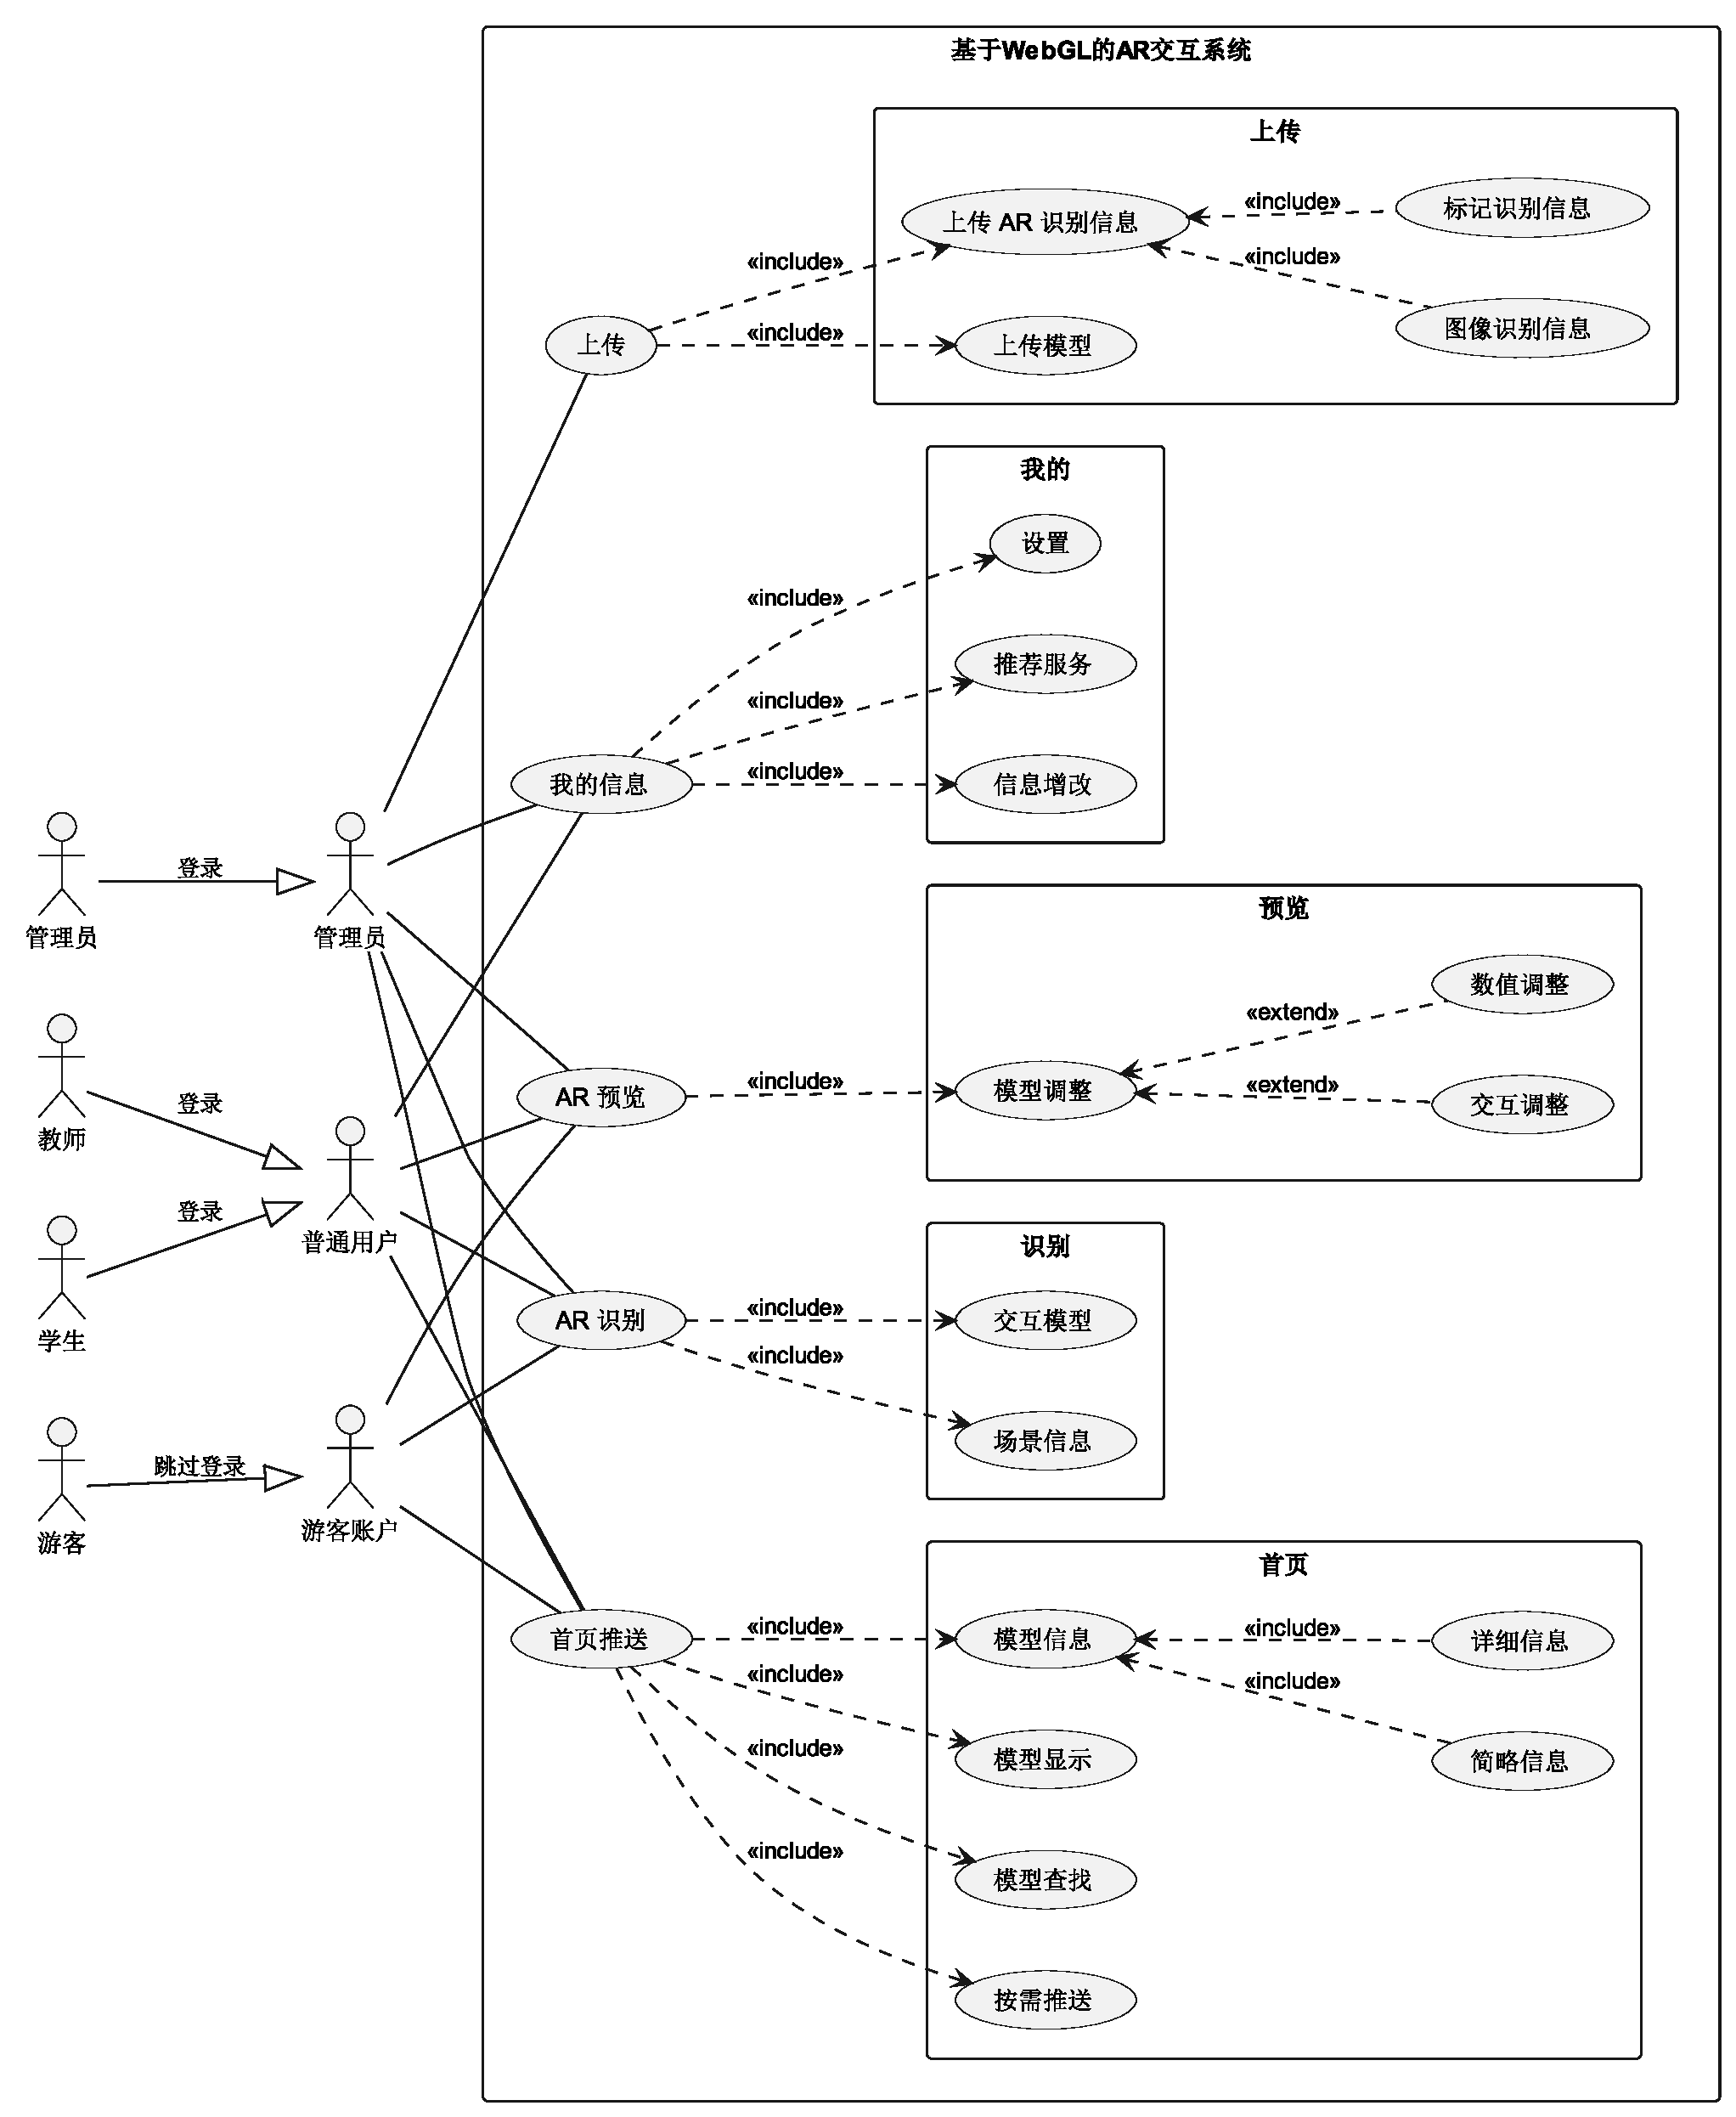
\includegraphics[width=\textwidth]{./figs/UserCase.eps}
  \caption{系统用例图}
  \label{fig:系统用例图}
\end{figure}


\subsubsection{功能性需求分析}

登陆注册: 用户 id 必须与学号或工作编号一致,在注册时匹配校园编号表。用户身份分为四类: 游客,学生,老师,管理员。游客账户为前端预留账户,用户可以通过该账户体验系统功能,但无法与后端进行交互。不同的身份将获得系统的不同权限以及推送内容。

用户的登录步骤如表\ref{table:用户登录用例表}所示:

\begin{table}[H]
  \centering
  \renewcommand\arraystretch{1.1}
  \small
  \caption{用户登录用例表}
  \label{table:用户登录用例表}
  \setlength{\tabcolsep}{4mm}
  \begin{tabular}{|p{2cm}|p{5.75cm}|p{5.75cm}|}
    \hline \textbf{用例名} & \multicolumn{2}{l|}{用户登录} \\
    \hline \textbf{角色} & \multicolumn{2}{l|}{学生,职工,管理员} \\
    \hline \textbf{准入条件} & \multicolumn{2}{l|}{用户拥有进入系统的权限} \\
    \hline \textbf{事件流} & \textbf{角色步骤} & \textbf{系统步骤} \\
    \hline \multirow{3}{*}{~} & \textbf{1.} 用户进入登录界面  &    \\
    \cline{2-3} & \textbf{2.} 用户输入用户名/邮箱和密码 & \textbf{3:} 前端进行数据检查。 \\
    \cline{2-3} &  & \textbf{4:} 后端查询数据库进行匹配。 \\
    \cline{2-3} &  & \textbf{5:} 用户进入系统,跳转到``首页''界面 \\
    \hline \textbf{退出条件}  & \multicolumn{2}{l|}{系统验证用户名密码正确} \\
    \hline \multirow{2}{*}{\textbf{例外}} & \multicolumn{2}{l|}{\textbf{1.} 步骤3,前端检查数据错误,给出提示信息。} \\
     & \multicolumn{2}{l|}{\textbf{2.} 步骤4,后端匹配数据失败,用户重新登录。} \\
    \hline
  \end{tabular}
\end{table}

新用户注册时需选择对应的身份,例如学生,教师等。系统将通过校园用户表自动判断用户与选择的权限组是否对应,用户注册步骤如表\ref{table:用户注册用例表}所示:

\begin{table}[H]
  \centering
  \renewcommand\arraystretch{1.1}
  \small
  \caption{用户注册用例表}
  \label{table:用户注册用例表}
  \setlength{\tabcolsep}{4mm}
  \begin{tabular}{|p{2cm}|p{5.75cm}|p{5.75cm}|}
    \hline \textbf{用例名} & \multicolumn{2}{l|}{用户注册} \\
    \hline \textbf{角色} & \multicolumn{2}{l|}{学生,职工,管理员} \\
    \hline \textbf{准入条件} & \multicolumn{2}{l|}{用户拥有进入系统的权限} \\
    \hline \textbf{事件流} & \textbf{角色步骤} & \textbf{系统步骤} \\
    \hline \multirow{3}{*}{~} & \textbf{1.} 用户进入注册界面。  &    \\
    \cline{2-3} & \textbf{2.} 用户填写并提交注册信息。 & \textbf{3:} 前端进行数据检查。 \\
    \cline{2-3} &  & \textbf{4:} 后端根据校园系统表判断能否注册,并返回信息。 \\
    \cline{2-3} &  & \textbf{5:} 前端显示注册结果,跳转到``我的''界面。 \\
    \hline \textbf{退出条件}  & \multicolumn{2}{l|}{用户成功注册} \\
    \hline \multirow{2}{*}{\textbf{例外}} & \multicolumn{2}{l|}{\textbf{1.} 步骤3,前端检查数据错误,给出提示信息。} \\
     & \multicolumn{2}{l|}{\textbf{2.} 步骤4,后端未匹配到对应编号,或编号与选定的权限组不符。} \\
    \hline
  \end{tabular}
\end{table}

在用户进入系统后,可在个人资料界面修改个人信息,修改用户信息步骤如表\ref{table:用户增改个人信息用例表}所示:

\begin{table}[H]
  \centering
  \renewcommand\arraystretch{1.1}
  \small
  \caption{用户增改个人信息用例表}
  \label{table:用户增改个人信息用例表}
  \setlength{\tabcolsep}{4mm}
  \begin{tabular}{|p{2cm}|p{5.75cm}|p{5.75cm}|}
    \hline \textbf{用例名} & \multicolumn{2}{l|}{用户增改个人信息} \\
    \hline \textbf{角色} & \multicolumn{2}{l|}{学生,职工,管理员} \\
    \hline \textbf{准入条件} & \multicolumn{2}{l|}{用户拥有个人账号} \\
    \hline \textbf{事件流} & \textbf{角色步骤} & \textbf{系统步骤} \\
    \hline \multirow{3}{*}{~} & \textbf{1.} 用户进入我的界面,针对个人信息进行增改。  &    \\
    \cline{2-3} & \textbf{2.} 用户提交修改后的个人信息。 & \textbf{3:} 前端进行数据检查。 \\
    \cline{2-3} &  & \textbf{4:} 后端增改数据 \\
    \cline{2-3} &  & \textbf{5:} 前端显示增改后的结果 \\
    \hline \textbf{退出条件}  & \multicolumn{2}{l|}{成功修改信息} \\
    \hline \multirow{2}{*}{\textbf{例外}} & \multicolumn{2}{l|}{\textbf{1.} 步骤3,前端检查数据错误,给出提示信息。} \\
     & \multicolumn{2}{l|}{\textbf{2.} 步骤4,后端增改数据失败,给出错误信息。} \\
    \hline
  \end{tabular}
\end{table}

首页推送: 系统首页划分为``为你推荐''、``最新更新''、 ``我的关注''三个分区,分别获取推荐内容,最新内容以及关注内容。用户选择不同分区时,系统将自动调用后端算法推送内容。首页推送功能执行步骤如表\ref{table:首页推送用例表}所示:

\begin{table}[H]
  \centering
  \renewcommand\arraystretch{1.1}
  \small
  \caption{首页推送用例表}
  \label{table:首页推送用例表}
  \setlength{\tabcolsep}{4mm}
  \begin{tabular}{|p{2cm}|p{5.75cm}|p{5.75cm}|}
    \hline \textbf{用例名} & \multicolumn{2}{l|}{首页推送} \\
    \hline \textbf{角色} & \multicolumn{2}{l|}{游客,学生,职工,管理员} \\
    \hline \textbf{准入条件} & \multicolumn{2}{l|}{用户能够进入系统} \\
    \hline \textbf{事件流} & \textbf{角色步骤} & \textbf{系统步骤} \\
    \hline \multirow{3}{*}{~} & \textbf{1.} 用户进入首页  &    \\
    \cline{2-3} & \textbf{2.} 用户选择 ``为你推荐'',``最新更新'',``我的关注'' 任一选项 & \textbf{3:} 前端发送对应请求 \\
    \cline{2-3} &  & \textbf{4:} 后端根据请求类型与权限组查找并返回不同数据。 \\
    \cline{2-3} &  & \textbf{5:} 前端根据接受的数据类型显示模型卡。 \\
    \hline \textbf{退出条件}  & \multicolumn{2}{l|}{用户切换筛选类型} \\
    \hline \multirow{1}{*}{\textbf{例外}} & \multicolumn{2}{l|}{\textbf{1.} 步骤4,后端查询数据失败。} \\
    \hline
  \end{tabular}
\end{table}

用户在首页也可自行查询相关内容,搜索栏支持按模型名称查询功能,系统后端返回结果后,前端会替换原先内容显示搜索的结果,首页查询功能的执行步骤如表\ref{table:首页查询用例表}所示:

\begin{table}[H]
  \centering
  \renewcommand\arraystretch{1.1}
  \small
  \caption{首页查询用例表}
  \label{table:首页查询用例表}
  \setlength{\tabcolsep}{4mm}
  \begin{tabular}{|p{2cm}|p{5.75cm}|p{5.75cm}|}
    \hline \textbf{用例名} & \multicolumn{2}{l|}{首页查询} \\
    \hline \textbf{角色} & \multicolumn{2}{l|}{游客,学生,职工,管理员} \\
    \hline \textbf{准入条件} & \multicolumn{2}{l|}{用户能够进入系统} \\
    \hline \textbf{事件流} & \textbf{角色步骤} & \textbf{系统步骤} \\
    \hline \multirow{3}{*}{~} & \textbf{1.} 用户进入首页  &    \\
    \cline{2-3} & \textbf{2.} 用户进行关键字搜索 & \textbf{3:} 前端检查搜索内容并发送对应请求 \\
    \cline{2-3} &  & \textbf{4:} 后端根据请求与权限组查找数据并返回。 \\
    \cline{2-3} &  & \textbf{5:} 前端根据接受的数据类型显示模型卡。 \\
    \hline \textbf{退出条件}  & \multicolumn{2}{l|}{用户点击``搜索''按钮} \\
    \hline \multirow{2}{*}{\textbf{例外}} & \multicolumn{2}{l|}{\textbf{1.} 步骤3,搜索内容出错。} \\
     & \multicolumn{2}{l|}{\textbf{2.} 步骤4,后端查询数据失败。} \\
    \hline
  \end{tabular}
\end{table}

3D 模型展示: 系统建立 3D 模型并展示环境,获取模型数据并在手机内直接展示,且提供模型背景,预设环境等可操作选项供用户预览。同时提供一定的模型文本信息,用户可以在简略信息与详细信息模式直接切换,也可完全屏蔽模型信息。模型展示功能的执行步骤如表\ref{table:模型展示用例表}所示:

\begin{table}[H]
  \centering
  \renewcommand\arraystretch{1.1}
  \small
  \caption{模型展示用例表}
  \label{table:模型展示用例表}
  \setlength{\tabcolsep}{4mm}
  \begin{tabular}{|p{2cm}|p{5.75cm}|p{5.75cm}|}
    \hline \textbf{用例名} & \multicolumn{2}{l|}{模型展示} \\
    \hline \textbf{角色} & \multicolumn{2}{l|}{游客,学生,职工,管理员} \\
    \hline \textbf{准入条件} & \multicolumn{2}{l|}{用户能够进入系统} \\
    \hline \textbf{事件流} & \textbf{角色步骤} & \textbf{系统步骤} \\
    \hline \multirow{3}{*}{~} & \textbf{1.} 用户进入首页  &    \\
    \cline{2-3} & \textbf{2.} 用户点击对应模型卡。 & \textbf{3:} 前端向后端请求模型详细信息数据。 \\
    \cline{2-3} &  & \textbf{4:} 后端返回模型数据。 \\
    \cline{2-3} &  & \textbf{5:} 前端加载界面与模型。 \\
    \cline{2-3} & \textbf{6:} 用户点击交互按钮。 & \textbf{7:} 前端做出对应响应。 \\
    \cline{2-3} & \textbf{8:} 用户退出``模型展示''界面 &  \\
    \hline \textbf{退出条件}  & \multicolumn{2}{l|}{用户退出``模型展示''界面} \\
    \hline \multirow{1}{*}{\textbf{例外}} & \multicolumn{2}{l|}{\textbf{1.} 步骤5,网络等问题加载模型或信息失败。} \\
    \hline
  \end{tabular}
\end{table}


3D 模型 AR 预览:系统调用设备摄像头将模型放入到 AR 环境中,允许用户在现实环境中对模型进行移动缩放等操作,提供 3D 模型预览服务。AR 预览功能的执行步骤如表\ref{table:AR 预览用例表}所示:

\begin{table}[H]
  \centering
  \renewcommand\arraystretch{1.1}
  \small
  \caption{AR 预览用例表}
  \label{table:AR 预览用例表}
  \setlength{\tabcolsep}{4mm}
  \begin{tabular}{|p{2cm}|p{5.75cm}|p{5.75cm}|}
    \hline \textbf{用例名} & \multicolumn{2}{l|}{AR 预览} \\
    \hline \textbf{角色} & \multicolumn{2}{l|}{游客,学生,职工,管理员} \\
    \hline \textbf{准入条件} & \multicolumn{2}{l|}{用户能够进入系统} \\
    \hline \textbf{事件流} & \textbf{角色步骤} & \textbf{系统步骤} \\
    \hline \multirow{3}{*}{~} & \textbf{1.} 用户进入``首页''界面。  &    \\
    \cline{2-3} & \textbf{2.} 用户点击模型卡并选择 AR 预览功能。 & \textbf{3:} 跳转至``预览''界面。 \\
    \cline{2-3} &  & \textbf{4:} 系统请求设备开启摄像头与 AR 服务。 \\
    \cline{2-3} &  & \textbf{5:} 向后端请求模型数据。 \\
    \cline{2-3} &  & \textbf{6:} 前端加载模型,展示 AR 预览界面。 \\
    \cline{2-3} & \textbf{7:} 用户操作 AR 预览界面 & \textbf{8:} 前端做出对应响应。 \\
    \cline{2-3} & \textbf{9:} 用户退出``AR 模型展示''界面。 &  \\
    \hline \textbf{退出条件}  & \multicolumn{2}{l|}{用户退出``AR 模型展示''界面。} \\
    \hline \multirow{2}{*}{\textbf{例外}} & \multicolumn{2}{l|}{\textbf{1.} 步骤4,系统请求摄像头权限或 AR 服务被拒。} \\
    & \multicolumn{2}{l|}{\textbf{2.} 步骤6,网络等问题加载模型或信息失败。} \\
    \hline
  \end{tabular}
\end{table}

AR 场景识别:根据摄像头捕捉的图像信息,采用标记捕捉或图像识别算法,在捕捉到对应信息后显示相关三维模型以及对应文本信息。AR 识别功能的执行步骤如表\ref{table:AR 识别用例表}所示:

\begin{table}[H]
  \centering
  \renewcommand\arraystretch{1.1}
  \small
  \caption{AR 识别用例表}
  \label{table:AR 识别用例表}
  \setlength{\tabcolsep}{4mm}
  \begin{tabular}{|p{2cm}|p{5.75cm}|p{5.75cm}|}
    \hline \textbf{用例名} & \multicolumn{2}{l|}{AR 识别} \\
    \hline \textbf{角色} & \multicolumn{2}{l|}{游客,学生,职工,管理员} \\
    \hline \textbf{准入条件} & \multicolumn{2}{l|}{用户能够进入系统} \\
    \hline \textbf{事件流} & \textbf{角色步骤} & \textbf{系统步骤} \\
    \hline \multirow{3}{*}{~} & \textbf{1.} 用户进入``识别''界面  & \textbf{2:} 系统请求设备开启摄像头与 AR 服务   \\
    \cline{2-3} &  & \textbf{3:} 系统根据地理位置按需加载识别信息。\\
    \cline{2-3} &  & \textbf{4:} 系统通过图像识别或标记捕捉算法实时匹配摄像头传输的场景信息。 \\
    \cline{2-3} &  & \textbf{5:} 捕捉到有效信息。显示模型或相关提示。 \\
    \cline{2-3} & \textbf{6:} 用户与系统交互 & \textbf{7:} 系统做出响应。 \\
    \cline{2-3} & \textbf{8:} 用户退出``AR 识别'界面  &  \\
    \hline \textbf{退出条件}  & \multicolumn{2}{l|}{用户退出``AR 识别''界面} \\
    \hline \multirow{2}{*}{\textbf{例外}} & \multicolumn{2}{l|}{\textbf{1.} 步骤2,系统请求摄像头权限或 AR 服务被拒。} \\
    & \multicolumn{2}{l|}{\textbf{2.} 步骤3,网络等问题加载模型或信息失败。} \\
    \hline
  \end{tabular}
\end{table}

\subsubsection{非功能性需求分析}

系统非功能性需求分析确保系统在满足功能需求的同时,也满足了非功能性需求,如性能、可靠性、安全性、可维护性等。确保满足非功能性需求可以有效保证软件稳定性、扩展性\cite{张宏升2011软件架构的非功能性需求指标和区域化支持}。

\begin{enumerate}
  \item 性能
  
  性能指标可分为时间性能和空间性能。
  \begin{itemize}
    \item 时间性能: 本系统操作的持续时间不超过2秒,数据连接操作的持续时间不超过5秒。系统利用浏览器异步加载机制加载需要的资源,采用非阻塞机制逐步对场景,模型加载。如果由于网络问题,数据无法获取,系统应在等待至多 10 分钟后给出提示并恢复。
    \item 空间性能: 本系统按需推送内容,在界面中每次仅推送有限内容,根据用户操作增加推送内容。在 AR 场景识别过程中,根据用户地理位置推送必要数据。
  \end{itemize}

  \item 可靠性
  
  本系统测试时间不少于20小时。在测试过程中,系统应尽可能经历所有可能出现的故障情况,以确保系统的成熟度。当硬件或软件出现异常时,系统仍应具有服务能力。业务容量减少,但不会导致系统崩溃。该系统应能在停机后十分钟内修复并正常运行。

  \item 可用性

  本系统在接收到用户输入的错误数据后,系统不会崩溃,系统能够识别错误并给用户相应的提示信息。系统界面美观,对用户具有吸引力。本系统的界面设计应在保证基本功能的基础上实现友好的布局,与市面上多数移动设备 app 界面操作保持一致。
  
  \item 易用性
  
  本系统易于学习。系统应确保操作逻辑符合常规 app 操作逻辑,新用户在第一次使用时,在3分钟的学习时间内了解整个系统的基本功能,在10分钟的学习时间内掌握系统的所有功能。AR交互系统的用户界面应该简单、直观、易于使用。系统采用合适的配色、布局和图标来吸引用户的注意力,并使用户能够快速、准确地完成任务。

  \item 安全性
  
  AR交互系统具有适当的安全措施,用户的隐私和数据安全。系统应该使用HTTPS协议来保护用户的数据传输。前端仅保留必要数据。后端对重要数据进行加密保存。

  \item 可维护性
  
  系统采用模块化设计。将系统拆分为多个独立的模块,每个模块处理特定的任务或功能。有助于提高系统的可维护性,开发人员可以更容易地定位和修复问题,并且在更新或升级时可以更轻松地进行更改。在系统设计和开发过程中,采用一致的编程规范和标准,确保代码的可读性和可维护性。使用版本控制工具(Git)提高系统可维护性。

  \item 可扩展性
  
  系统中的各个模块应该尽可能地松耦合,以避免修改一个模块对其他模块产生意外影响。这有助于确保系统的可拓展性和稳定性。在设计和开发过程中,使用广泛采用的标准和技术,以便将来可以轻松地添加新功能或集成其他系统。
\end{enumerate}
\section{系统设计}

系统设计是指在软件开发过程中,对整个系统进行设计和规划,包括对系统的架构、组件、模块、数据库、接口、协议、算法等各方面的设计。系统设计是将用户需求转化为可实现的系统的过程。本文将从系统总体设计开始,继而阐述基础功能设计,着重阐述核心功能设计。

\subsection{系统总体设计}

\subsubsection{系统架构设计}

系统基于 B/S 架构开发,核心功能位于浏览器端,后端仅提供必要的数据服务。用户通过浏览器端发起数据请求,服务器端负责处理请求后返回必要数据,浏览器再通过核心的 WebGL 与 AR 技术展示结果。

本系统的整体设计架构如图\ref{fig:系统架构设计图}所示:

\begin{figure}[H]
  \small
  \centering
  \begin{tikzpicture}[font=\small]
    \begin{scope}[xshift=-1cm, yshift=0.25cm]
      \node [block, color=white, fill=blue!60] (user) at (-2,0) {用户};
      \node [block, color=white, fill=blue!60] (device) at (0,0) {移动设备};
      \draw [-Stealth] (user) -- (device);
    \end{scope}
    \node  at (4.5,2.3) {系统};
    \node [draw=black, dashed, minimum width=6cm, minimum height=4.5cm] (front) at (4.5,0.5) {};
    \begin{scope}[xshift=2.75cm]
      \node [draw=orange, dashed, minimum width=2cm, minimum height=3.5cm] (front) at (0,0.25) {};
      \node [font=\footnotesize] at (0,1.7) {前端};
      \node [block, color=white, fill=orange!60] at (0,1) {前端模块};
      \node [block, color=white, fill=orange!60] at (0,0) {前端模块};
      \node [block, color=white, fill=orange!60] at (0,-1) {前端模块};
      \node [block, color=white, fill=green!60!black] (cos) at (0,3.5) {COS 存储桶};
    \end{scope}
    \begin{scope}[xshift=6.25cm]
      \node [draw=red, dashed, minimum width=2cm, minimum height=3.5cm] (back) at (0,0.25) {};
      \node [font=\footnotesize] at (0,1.7) {后端};
      \node [block, color=white, fill=red!60] at (0,1) {后端接口};
      \node [block, color=white, fill=red!60] at (0,0) {后端接口};
      \node [block, color=white, fill=red!60] at (0,-1) {后端接口};
      \node [block, color=white, fill=red!60] (terminalDevice) at (0,3.5) {终端设备};
      \draw [Stealth-Stealth] (terminalDevice) -- (back);
    \end{scope}
    \begin{scope}[xshift=10cm, yshift=0.25cm]
      \node [block, color=white, fill=green!60!black] (mysql) at (0,0) {MySql};
    \end{scope}
    \begin{scope}[xshift=4.5cm, yshift=-3cm]
      \node at (0,0.75) {语言与框架支持};
      \node [block, color=white, fill=orange!60] at (-1.5,0) {JS, TS, React};
      \node [block, color=white, fill=red!60] at (1.5,0) {Java, SpringBoot};
    \end{scope}
    \draw [-Stealth] (device) -- (front) node [midway, above, font=\footnotesize] {访问};
    \draw [Stealth-Stealth] (front) -- (back) node [midway, above, font=\footnotesize] {请求响应};
    \draw [Stealth-Stealth] (back) -- (mysql) node [midway, above, font=\footnotesize] {业务读写};
    \draw [Stealth-] (front) -- (cos) node [pos=0.4, font=\footnotesize] {模型,图形数据读取};
  \end{tikzpicture}
  \caption{系统架构设计图}
  \label{fig:系统架构设计图}
\end{figure}

\subsubsection{系统技术选择}

在技术选择的过程中,需要考虑技术适用性,开发难度,成本,社区生态,安全性,可维护性。综合考量,本系统使用如下主流技术。

前端采用 React 框架,该框架能带来诸多优势。例如组件化开发,可以将 AR 组件和 WebGL 组件封装成可复用的组件,便于开发和维护。这样可以提高开发效率,减少代码重复。虚拟 DOM 技术可以实现高效的页面渲染和更新。在 AR 校园交互系统中,不同的 AR 场景需要不断地更新,React 可以通过虚拟 DOM 技术帮助我们快速更新渲染。React 生态系统有许多开源库和工具,可以帮助我们更快地开发 AR 校园交互系统。例如,React Three Fiber 可以将 React 和 Three.js 集成起来,帮助我们更容易地实现 3D 场景和特效。React 提供了一种清晰的数据流管理方式,即单向数据流。在 AR 校园交互系统中,我们可以将 AR 组件和 WebGL 组件所需要的数据通过 props 传递到组件中,这样可以更好地管理组件之间的数据流动。在 React 作为前端骨干框架的基础上,前端还是用到了如下组件:
\begin{itemize}
  \item MaterialUI: 提供响应式UI组件,具备极佳的动画效果与样式自定义系统。
  \item Redux: 提供公有数据的统一管理,便于 vDOM 中各个层级组件之间交互数据。
  \item Vite: 新一代打包工具,具备按需加载,快速响应等优点。
  \item fetch: ES6 提供的 http 请求 API。浏览器原生支持,无需额外封装 HttpRequest 请求。
\end{itemize}

后端框架采用 SpringBoot 框架,SpringBoot 框架可以快速构建应用程序,并且可以使用自动配置功能快速集成各种库和服务。这意味着可以更快地开发出高效、可靠的后端应用程序。强大的生态系统:SpringBoot 框架有着庞大的生态系统,拥有许多插件和第三方库,可以帮助开发人员更好地开发应用程序。在 SpringBoot 作为核心后端框架的基础上,后端还用到了如下组件:
\begin{itemize}
  \item Spring Data JPA: 全 ORM 框架,能够非常方便快捷地与 SpringBoot 框架融合,提供了便捷的操作数据库的接口。
  \item MySQL: 免费开源的关系型数据库,拥有企业级数据处理速度。
\end{itemize}

在核心功能上,WebGL 采用 three.js 组件实现,考虑到前端主要框架是 React,因此采用 @react-three 组件,使用 JSX 语法进行开发。@react-three 可以完美融合进 React 框架,可以轻松地与 React,Redux,MaterialUI 集成。@react-three 可以通过 React 组件化的思路来创建 3D 场景。开发者可以使用熟悉的 React API 来管理 3D 对象和动画,并可以在 React 应用中轻松地嵌入 Three.js 场景,从而简化了开发流程。AR 功能则采用 ar.js 组件,由于该组件无法直接通过 JSX 语法嵌入 React 组件,系统为其添加了 ts 类型并进一步封装成 JSX 组件。

\subsubsection{功能模块设计}

系统的模块可大致划分为: 基础功能模块,核心功能模块。其中基础功能模块包括登陆注册,用户权限管理,数据请求筛选等功能。核心功能模块利用 WebGL 与 AR 技术打造交互系统。其中 WebGL 功能模块以 WebGL 技术为核心,采用 three.js 组件实现 3D 模型的展示与交互功能。AR 功能模块以 WebGL 技术为基础,以 ar.js 为核心,采用图像识别与标记捕捉算法捕捉摄像机图像数据完成增强现实功能。功能模块的结构图如图\ref{fig:功能模块结构图}所示:

\begin{figure}[H]
  \small
  \centering
  \begin{tikzpicture}[font=\small]
    \node [draw] (whole) at (0,1.5) {基于 WebGL 的 AR 校园交互系统};
    \begin{scope}[xshift=-3cm]
      \node [draw] (basic) at (0,0) {基础功能};
      \node [draw] (user) at (-2,-1.5) {用户认证};
      \node [draw] (screen) at (0,-1.5) {数据推送};
      \node [draw] (update) at (2,-1.5) {数据上传};
      \node [draw, text width=1em, text centered] (login) at (-2.75,-3.5) {登录功能};
      \node [draw, text width=1em, text centered] (registry) at (-2,-3.5) {注册功能};
      \node [draw, text width=1em, text centered] (info) at (-1.25,-3.5) {信息增改};
      \node [draw, text width=1em, text centered] (push) at (-0.375,-3.5) {模型推送};
      \node [draw, text width=1em, text centered] (search) at (0.375,-3.5) {模型查询};
      \node [draw, text width=1em, text centered] (model) at (1.625,-3.5) {模型上传};
      \node [draw, text width=1em, text centered] (arData) at (2.375,-3.5) {ar数据上传};
    \end{scope}
    \begin{scope}[xshift=3cm]
      \node [draw] (core) at (0,0) {核心功能};
      \node [draw] (webgl) at (-1,-1.5) {WebGL};
      \node [draw] (ar) at (1,-1.5) {AR};
      \node [draw, text width=1em, text centered] (showModel) at (-1.375,-3.5) {模型展示};
      \node [draw, text width=1em, text centered] (operateModel) at (-0.625,-3.5) {模型操作};
      \node [draw, text width=1em, text centered] (arPreview) at (0.625,-3.5) {场景预览};
      \node [draw, text width=1em, text centered] (arIdentify) at (1.375,-3.5) {场景识别};
    \end{scope}
    \draw (whole) -- ++(0,-0.75) -| (basic);
    \draw (whole) -- ++(0,-0.75) -| (core);
    \draw (basic) -- ++(0,-0.75) -| (user);
    \draw (basic) -- ++(0,-0.75) -| (screen);
    \draw (basic) -- ++(0,-0.75) -| (update);
    \draw (core) -- ++(0,-0.75) -| (webgl);
    \draw (core) -- ++(0,-0.75) -| (ar);
    \draw (user) -- ++(0,-0.5) -| (login);
    \draw (user) -- ++(0,-0.5) -| (registry);
    \draw (user) -- ++(0,-0.5) -| (info);
    \draw (screen) -- ++(0,-0.5) -| (push);
    \draw (screen) -- ++(0,-0.5) -| (search);
    \draw (update) -- ++(0,-0.5) -| (model);
    \draw (update) -- ++(0,-0.5) -| (arData);
    \draw (webgl) -- ++(0,-0.5) -| (showModel);
    \draw (webgl) -- ++(0,-0.5) -| (operateModel);
    \draw (ar) -- ++(0,-0.5) -| (arPreview);
    \draw (ar) -- ++(0,-0.5) -| (arIdentify);
  \end{tikzpicture}
  \caption{功能模块结构图}
  \label{fig:功能模块结构图}
\end{figure}

\subsubsection{数据库设计}

系统将文本数据存储在关系型数据库 MySQL 中,非文本数据(图像,模型等)存储在 COS 对象存储桶中。本系统共需标记表,标记信息表,模型表,学校人员表,用户表,收藏表,粉丝表,关注表共九张表。各表介绍如下:
\begin{itemize}
  \item 标记表: 记录 AR 识别的标记信息。数据段包括标记类型,标记图像类型,标记图像对应 URL,前端需要显示的模型 Id,标记信息 Id 等。通过这个表系统将实时匹配摄像头传输来的信息进行图像匹配,匹配成功后根据对应模型 Id 或信息 Id 显示内容。
  \item 标记信息表: 记录对应标记的信息。主要记录标记物的信息,如物品名称,简要介绍,上传作者等。前端通过该表在匹配到标记后显示对应标记的信息。
  \item 模型表: 记录 3D 模型信息,包括模型 URL, 模型信息等。前端通过该表显示对应模型及相关信息。
  \item 模型控制表: 记录 3D 模型控制信息,影响显示时的场景设置,包括自旋速度,环境背景等。前端通过读取该表控制模型与环境。
  \item 模型点赞表: 记录模型被点赞的信息。
  \item 学校人员表: 学校教职工,学生信息表。
  \item 用户表: 记录用户信息,包括权限组,昵称,所属部门等。
  \item 用户收藏表: 记录用户收藏的模型内容。
  \item 用户关注表: 记录用户的关注用户数据。
\end{itemize}

各数据表的详细字段信息如下:

标记表记录图像识别标记信息,其中标记类型 (marker\_type) 分为常规标记(common)与区域标记(area)。所有常规标记都将一次性传输到用户设备中进行匹配,区域标记仅当用户设备定位达到条件时进行传输。标记文件类型(file\_type)对应图像识别或标记捕捉文件的类型。该表完整字段如表\ref{table:标记表}所示:

\begin{table}[H]
  \centering
  \small
  \caption{标记表}
  \label{table:标记表}
  \setlength{\tabcolsep}{3.7mm}
  \begin{tabular}{l|l|c|l}
    \toprule
    \textbf{字段名称} & \textbf{字段类型} & \textbf{非空} & \textbf{描述} \\
    \midrule
    id & bigint & √ & 主键,自增。 \\
    marker\_type & Enum(`common',`area') & √ & 标记类型, 常规标记或区域标记。 \\
    file\_type & Enum(`pattern',`barcode',`nft') & √ & 标记文件类型,对应标记文件的格式。 \\
    file\_url & varchar(255) & √ & 标记或图像对应的 URL。 \\
    info\_id & bigint & × & 需要显示的标记信息, 对应标记信息表 id。 \\
    model\_id & bigint & × & 需要显示的模型 id, 对应模型表 id。 \\
    author\_id & bigint & × & 标记上传者的 id, 对应用户表 id。 \\
    create\_time & datetime & √ & 标记创建的时间。 \\
    update\_time & datetime & √ & 标记更新的时间。 \\
    \bottomrule
  \end{tabular}
\end{table}

标记信息表记录对应标记的信息数据, 主要存储标记的文字介绍信息,该表完整字段如表\ref{table:标记信息表}所示:

\begin{table}[H]
  \centering
  \small
  \caption{标记信息表}
  \label{table:标记信息表}
  \setlength{\tabcolsep}{8mm}
  \begin{tabular}{l|l|c|l}
    \toprule
    \textbf{字段名称} & \textbf{字段类型} & \textbf{非空} & \textbf{描述} \\
    \midrule
    id & bigint & √ & 主键,自增。 \\
    cover\_url & varchar(255) & √ & 标记信息的封面图。 \\
    title & varchar(20) & √ & 标记的名称或标题。 \\
    abstract& varchar(255) & √ & 标记的简介。 \\
    introduction & varchar(65535) & × & 标记的详细信息。 \\
    author\_id & bigint & × & 标记上传者的 id, 对应用户表 id。 \\
    location & varchar(20) & × & 标记对应的地理位置。 \\
    create\_time & datetime & √ & 标记创建的时间。 \\
    update\_time & datetime & √ & 标记更新的时间。 \\
    \bottomrule
  \end{tabular}
\end{table}

模型表用于记录模型URL与相关数据信息,该表完整字段如表\ref{table:模型表}所示:

\begin{table}[H]
  \centering
  \small
  \caption{模型表}
  \label{table:模型表}
  \setlength{\tabcolsep}{10.2mm}
  \begin{tabular}{l|l|c|l}
    \toprule
    \textbf{字段名称} & \textbf{字段类型} & \textbf{非空} & \textbf{描述} \\
    \midrule
    id & bigint & √ & 主键,自增。 \\
    cover\_url & varchar(255) & √ & 模型的封面图。 \\
    title & varchar(20) & √ & 模型的名称。 \\
    like\_count & varchar(20) & √ & 模型被喜欢的人数。 \\
    abstract & varchar(255) & √ & 模型的介绍。 \\
    model\_url & varchar(255) & √ & 模型存储的地址。 \\
    control\_id & bigint & × & 模型控制表 id。 \\
    create\_time & datetime & √ & 模型创建的时间。 \\
    update\_time & datetime & √ & 模型更新的时间。 \\
    \bottomrule
  \end{tabular}
\end{table}

模型控制表用于存储模型与环境的配置信息,由于控制信息仅在模型预览时会被使用,在 AR 预览与 AR 识别时仅需提供模型的基本信息即可,因此将模型表与模型控制表分离。该表完整字段如表\ref{table:模型控制表}所示:

\begin{table}[H]
  \centering
  \small
  \caption{模型控制表}
  \label{table:模型控制表}
  \setlength{\tabcolsep}{6.3mm}
  \begin{tabular}{l|l|c|l}
    \toprule
    \textbf{字段名称} & \textbf{字段类型} & \textbf{非空} & \textbf{描述} \\
    \midrule
    id & bigint & √ & 主键,自增。 \\
    auto\_rotate\_speed & int & × & 模型自动旋转速度。 \\
    background & boolean & × & 模型是否需要环境背景。 \\
    preset & Enum(`sunset', `dawn',...) & × & 模型使用的环境背景。 \\
    blur & number & × & 环境背景模糊程度。 \\
    float\_speed & number & × & 模型浮动效果速度。 \\
    rotation\_intensity & number & × & 模型浮动时自旋速度。 \\
    float\_intensity & number & × & 模型浮动强度。 \\
    create\_time & datetime & √ & 模型控制信息创建的时间。 \\
    update\_time & datetime & √ & 模型控制信息更新的时间。 \\
    \bottomrule
  \end{tabular}
\end{table}

模型点赞表用于记录点赞用户与模型之间的关系。主要用于计算模型被点赞数,防止同一用户多次点赞。该表完整字段如表\ref{table:模型点赞表}所示:

\begin{table}[H]
  \centering
  \small
  \caption{模型点赞表}
  \label{table:模型点赞表}
  \setlength{\tabcolsep}{9mm}
  \begin{tabular}{l|l|c|l}
    \toprule
    \textbf{字段名称} & \textbf{字段类型} & \textbf{非空} & \textbf{描述} \\
    \midrule
    id & bigint & √ & 主键,自增。 \\
    user\_id & bigint & √ & 点赞用户 id,对应用户表主键。 \\
    model\_id & bigint & √ & 模型 id,对应模型表主键。 \\
    create\_time & datetime & √ & 点赞时间。 \\
    \bottomrule
  \end{tabular}
\end{table}

学校人员表记录学生与教职工的信息,该表主要模拟学校的人员信息表,在实际使用中,系统需要对接的人员表字段要多于本表,本表只提供系统必要的字段。该表完整字段如表\ref{table:学校人员表}所示:

\begin{table}[H]
  \centering
  \small
  \caption{学校人员表}
  \label{table:学校人员表}
  \setlength{\tabcolsep}{6mm}
  \begin{tabular}{l|l|c|l}
    \toprule
    \textbf{字段名称} & \textbf{字段类型} & \textbf{非空} & \textbf{描述} \\
    \midrule
    id & bigint & √ & 主键,自增。 \\
    identity & Enum(`student',`teacher',`staff',...) & √ & 人员身份。 \\
    real\_name & varchar(20) & √ & 真实姓名。 \\
    id\_number & char(18) & √ & 身份证号。 \\
    create\_time & datetime & √ & 人员信息创建的时间。 \\
    update\_time & datetime & √ & 人员信息更新的时间。 \\
    \bottomrule
  \end{tabular}
\end{table}

用户表记录系统用户的详细信息,用户表数据在创建时需查验学校人员表。该表完整字段如表\ref{table:用户表}所示:

\begin{table}[H]
  \centering
  \small
  \caption{用户表}
  \label{table:用户表}
  \setlength{\tabcolsep}{4.2mm}
  \begin{tabular}{l|l|c|l}
    \toprule
    \textbf{字段名称} & \textbf{字段类型} & \textbf{非空} & \textbf{描述} \\
    \midrule
    id & bigint & √ & 主键,自增。 \\
    name & varchar(20) & √ & 用户昵称。 \\
    avatar\_url & varchar(255) & × & 用户头像 url。 \\
    sexual & Enum(`male', `female', `secret', `undefined') & √ & 用户性别。 \\
    permission & Enum(`student', `teacher', `admin', `visitor') & √ & 用户所属权限组。 \\ 
    college & varchar(255) & × & 用户所属学院。 \\
    department & varchar(255) & × & 用户所属部门,专业。 \\
    signature & varchar(255) & × & 用户个性签名。 \\
    tags & varchar(255) & × & 用户身份标签。 \\
    create\_time & datetime & √ & 用户信息创建的时间。 \\
    update\_time & datetime & √ & 用户信息更新的时间。 \\
    \bottomrule
  \end{tabular}
\end{table}

用户收藏表用于记录用户与被收藏模型之间的关系。用于向用户提供快速访问收藏模型服务。该表完整字段如表\ref{table:用户收藏表}所示:

\begin{table}[H]
  \centering
  \small
  \caption{用户收藏表}
  \label{table:用户收藏表}
  \setlength{\tabcolsep}{9mm}
  \begin{tabular}{l|l|c|l}
    \toprule
    \textbf{字段名称} & \textbf{字段类型} & \textbf{非空} & \textbf{描述} \\
    \midrule
    id & bigint & √ & 主键,自增。 \\
    user\_id & bigint & √ & 用户 id,对应用户表主键。 \\
    model\_id & bigint & √ & 模型 id,对应模型表主键。 \\
    create\_time & datetime & √ & 收藏时间。 \\
    \bottomrule
  \end{tabular}
\end{table}

用户关注表用于记录用户之间的关注关系。该表完整字段如表\ref{table:用户关注表}所示:

\begin{table}[H]
  \centering
  \small
  \caption{用户关注表}
  \label{table:用户关注表}
  \setlength{\tabcolsep}{9mm}
  \begin{tabular}{l|l|c|l}
    \toprule
    \textbf{字段名称} & \textbf{字段类型} & \textbf{非空} & \textbf{描述} \\
    \midrule
    id & bigint & √ & 主键,自增。 \\
    user\_id & bigint & √ & 被关注者 id,对应用户表主键。 \\
    follower\_id & bigint & √ & 关注者 id,对应模型表主键。 \\
    create\_time & datetime & √ & 关注时间。 \\
    \bottomrule
  \end{tabular}
\end{table}

\subsection{基础功能详细设计}

\subsubsection{用户认证}

用户认证模块包含用户注册,用户登录,用户信息增改三个主要功能。

系统将对重要数据进行加密存储与加密传输,在数据库中使用 AES 算法加密,在前后端传输过程中使用 RSA 双向加密算法加密。系统将先在前端进行数据检查,主要检查数据格式,权限。无误后再传输到后端进行查数据库匹配。

用户注册依赖于已有的学校人员信息表,仅匹配到对应的数据(id, 身份证号)后允许注册,并根据人员身份赋予对应的权限组。

整个用户认证模块涉及到的主要界面与所有数据表包括:
\begin{itemize}
  \item 界面: 登陆界面,注册界面,``我的''界面。
  \item 数据表: 学校人员表, 用户表, 用户收藏表, 用户关注表。
\end{itemize}

用户认证模块整体操作的顺序图如图\ref{fig:用户认证顺序图}所示:

\begin{figure}[H]
  \small
  \centering
  \begin{sequencediagram}
    \newthread{user}{:User}
    \newinst[2]{b}{:Browser}
    \newinst[3]{s}{:Server}
    \newinst[2]{mysql}{:MySQL}
    \begin{call}{user}{输入认证数据}{b}{认证成功}
      \begin{call}{b}{前端数据检查}{b}{通过检查}
        \begin{sdblock}{Alt}{前端数据检查失败}
          \mess{b}{要求重新输入数据}{user}
        \end{sdblock}
      \end{call}
      \begin{call}{b}{RSA 加密传输数据}{s}{后端认证成功}
        \postlevel
        \begin{call}{s}{\shortstack{查表: 用户表,\\学校人员表}}{mysql}{验证数据与权限}
        \end{call}
        \begin{call}{s}{验证成功}{mysql}{AES 加密存储用户数据}
        \end{call}
        \begin{sdblock}{Alt}{后端验证失败}
          \mess{s}{返回错误信息}{b}
          \mess{b}{要求重新输入数据}{user}
        \end{sdblock}
      \end{call}
    \end{call}
  \end{sequencediagram}
  \caption{用户认证顺序图}
  \label{fig:用户认证顺序图}
\end{figure}

\subsubsection{数据推送}

数据推送模块包括模型推送与模型查询两个主要功能。

模型推送根据用户在``主页''界面的分区选择: ``为你推荐'', ``最新更新'', ``我的关注''。推送相关内容。三个分区对应后端三种不同的算法:
\begin{itemize}
  \item 为你推荐: 推送点赞数较高的模型。
  \item 最新更新: 推送最新更新的模型。
  \item 我的关注: 推荐用户关注的用户发布的模型。
\end{itemize}

模型查询根据模型名称查询数据库字段并返回相应内容。整个数据推送模块涉及到的主要界面与所有数据表包括:
\begin{itemize}
  \item 界面: ``首页'' 界面。
  \item 数据表: 模型表,用户表,模型点赞表,用户关注表,用户收藏表。
\end{itemize}

数据推送模块整体操作的顺序图如图\ref{fig:数据推送顺序图} 所示:

\begin{figure}[H]
  \small
  \centering
  \begin{sequencediagram}
    \newthread{user}{:User}
    \newinst[2]{b}{:Browser}
    \newinst[3]{s}{:Server}
    \newinst[2]{mysql}{:MySQL}
    \begin{call}{user}{用户选择偏好}{b}{返回对应模型卡}
      \begin{call}{b}{前端传输用户偏好数据}{s}{后端返回数据}
        \begin{call}{s}{根据偏好选择对应算法}{s}{数据处理}
          \postlevel \postlevel
          \begin{call}{s}{\shortstack{查表: 模型表,用户表, \\模型点赞,用户关注表}}{mysql}{返回对应数据}
          \end{call}
        \end{call}
      \end{call}
    \end{call}
  \end{sequencediagram}
  \caption{数据推送顺序图}
  \label{fig:数据推送顺序图}
\end{figure}

\subsubsection{数据上传}

数据上传模块包括模型上传与 ar 数据上传两个主要功能。

模型上传功能以 3D 模型为核心,目前仅支持 glb 格式的模型,且需要用户另行存储模型数据,系统通过 url 在前端获取模型。ar 数据上传以识别数据为核心,目前支持图像识别,patt 格式的标记捕捉。

整个数据上传模块涉及到的主要界面与所有数据表包括:
\begin{itemize}
  \item 界面: ``上传'' 界面。
  \item 数据表: 标记表,标记信息表,模型表,模型控制表。
\end{itemize}

数据上传模块整体操作的顺序图如图\ref{fig:数据上传顺序图} 所示:

\begin{figure}[H]
  \small
  \centering
  \begin{sequencediagram}
    \newthread{user}{:User}
    \newinst[2]{b}{:Browser}
    \newinst[3]{s}{:Server}
    \newinst[2]{mysql}{:MySQL}
    \begin{call}{user}{输入上传数据}{b}{上传成功}
      \begin{call}{b}{前端权限验证与数据检查}{b}{通过检查}
        \begin{sdblock}{Alt}{前端数据检查失败}
          \mess{b}{要求重新输入数据}{user}
        \end{sdblock}
      \end{call}
      \begin{call}{b}{传输数据}{s}{后端上传成功}
        \postlevel
        \begin{call}{s}{\shortstack{操作表: 标记表,模型表,\\标记信息表,模型控制表}}{mysql}{操作完成}
        \end{call}
        \begin{sdblock}{Alt}{写入表失败}
          \mess{s}{返回错误信息}{b}
          \mess{b}{给出错误提示}{user}
        \end{sdblock}
      \end{call}
    \end{call}
  \end{sequencediagram}
  \caption{数据上传顺序图}
  \label{fig:数据上传顺序图}
\end{figure}

\subsection{核心功能详细设计}

系统的核心功能位于前端,这小节会详细说明前端各个组件之间如何协作完成核心功能,涉及到的组件包括:
\begin{itemize}
  \item @ar-js-org/ar.js: AR 功能核心组件,用于进行图象识别或标记捕捉,下文简称 ar.js
  \item react: 前端主要框架。
  \item @reduxjs/toolkit: 状态管理组件,下文简称 redux。
  \item leva: 控制板交互组件,允许用户通过 UI 修改数据。
  \item three: three.js, WebGL 技术的具体实现。
  \item @react-three/fiber: 在 react 框架基础上对 three.js 的封装,采用了 jsx 语法, 下文 three.js 具体实现上采用的是该组件。
  \item @react-three/drei: 基于 @react-three/fiber, 提供了预设环境,下文简称 drei。
  \item @react-three/xr: 基于 @react-three/fiber, 封装了 three.js 的 XR(包括 AR) 功能,下文简称 xr。
\end{itemize}

\subsubsection{WebGL 模块}

WebGL 模块能够显示三维物体,并且能通过触摸或修改控制板数据的方式操作三维物体与对应的环境。主要包括模型显示,模型操作功能。

系统在接受到模型数据后,会首先创建对应的界面,显示模型信息,在控制板中显示可操作的数据。由于模型数据较大,系统将异步请求模型数据。系统可通过悬浮按钮的诸多选项调整界面模式,例如: 屏蔽信息卡,关注于模型本身。

WebGL 模块被化拆分为如下具体功能模块:
\begin{itemize}
  \item 控制模块: 配置模型控制信息,采用 drei 组件的轨道控制器(OrbitControls),用户可以通过滑动,双指放大等操作与模型交互。
  \item 环境模块: 配置模型虚拟环境信息,采用 drei 组建的环境组件(Environment),预设自然环境为落日,可提供模型控制表配置。
  \item 浮动模块: 操作物体浮动状态,使得物体可以自旋,上下浮动,达到更好的展示效果,可提供模型控制表配置。
  \item 光照模块: 提供环境光与阴影效果,可提供模型控制表配置。
  \item 网格模块: 通过网络请求获取模型本身。
\end{itemize}

此外,用户也可以通过 leva 控制板修改环境模块,浮动模块,光照模块数据,进而操作模型。

整个WebGL模块涉及到的主要界面与所有数据表包括:
\begin{itemize}
  \item 界面: ``模型预览'' 界面,``AR预览'' 界面,``AR识别'' 界面。
  \item 数据表: 模型表,模型控制表,模型点赞表。
\end{itemize}

WebGL 模块中前端各关键模块协作关系如图\ref{fig:WebGL 模块协作关系}所示:

\begin{figure}[H]
  \small
  \centering
  \begin{tikzpicture}[font=\small]
    \begin{scope}[xshift=-5cm]
      \node [block, color=white, fill=green!60!black] (user) at (0,0) {用户};
    \end{scope}
    \begin{scope}
      \node [block, color=white, fill=orange] (leva) at (-2,0.5) {控制板};
      \node [block, color=white, fill=blue!60] (control) at (-2,-0.5) {控制模块};
      \node [block, color=white, fill=blue!60] (environment) at (2,1.5) {环境模块};
      \node [block, color=white, fill=blue!60] (float) at (2,0.5) {浮动模块};
      \node [block, color=white, fill=blue!60] (light) at (2,-0.5) {光照模块};
      \node [block, color=white, fill=blue!60] (mesh) at (2,-1.5) {网格模块};
    \end{scope}
    \begin{scope}[xshift=5cm]
      \node [block, color=white, fill=red] (back) at (0,0.5) {后端};
      \node [block, color=white, fill=red] (mysql) at (3,0.5) {MySQL};
      \node [block, color=white, fill=red] (cos) at (3,-1) {COS};
    \end{scope}
    \draw [-Stealth] (user) -- (leva) node [font=\footnotesize, midway, above] {修改数据};
    \draw [-Stealth] (user) -- (control) node [font=\footnotesize, midway, below] {触摸操作};
    \draw [-Stealth] (leva) -- (environment) node [font=\footnotesize, midway, above] {修改参数};
    \draw [-Stealth] (leva) -- (float) node [font=\footnotesize, midway, above] {修改参数};
    \draw [-Stealth] (leva) -- (light) node [font=\footnotesize, midway, below] {修改参数};
    \draw [-Stealth] (control) -- (mesh) node [font=\footnotesize, midway, below] {影响模型};
    \draw [-Stealth] (back) -- (environment) node [font=\footnotesize, midway, above] {初始化参数};
    \draw [-Stealth] (back) -- (float) node [font=\footnotesize, midway, above] {初始化参数};
    \draw [-Stealth] (back) -- (light) node [font=\footnotesize, midway, above] {初始化参数};
    \draw [-Stealth] (back) -- (mesh) node [font=\footnotesize, midway, below] {提供模型数据};
    \draw [-Stealth] (back) -- (mysql) node [font=\footnotesize, midway, above] {读取数据};
    \draw [Stealth-Stealth] (cos) -- (mesh) node [font=\footnotesize, midway, above] {加载模型};
  \end{tikzpicture}
  \caption{WebGL 模块协作关系}
  \label{fig:WebGL 模块协作关系}
\end{figure}

\subsubsection{AR 模块}

AR 模块在 WebGL 模块基础上引入 AR 功能,通过图像识别与标记捕捉的方法实时解析摄像头传输的图像信息并作出响应。主要包括场景预览与场景识别功能。

系统在进入 AR 模块后,会首先获取摄像头权限并显示现实场景。在场景预览功能中,将虚拟物体投射到真实场景中,用户可以通过仪表盘或触摸操作调整模型。在场景识别功能中,系统会调用 ar.js 提供的识别功能捕捉图像信息,在成功捕捉到信息后,屏幕将会显示对应的 3D 模型或标记信息。

AR 模块在 WebGL 模块基础上进行了以下修改:
\begin{itemize}
  \item AR 网格模块: 允许用户通过控制板对模型进行缩放,旋转等操作。
  \item AR 控制模块: 提供辅助坐标轴,允许用户触摸屏幕对模型进行缩放,旋转等操作。
  \item AR 识别模块: 整合 ar.js 的识别功能。
\end{itemize}

AR 模块各关键模块协作关系如图\ref{fig:AR 模块协作关系}所示:

\begin{figure}[H]
  \small
  \centering
  \begin{tikzpicture}[font=\small]
    \begin{scope}[xshift=-3cm]
      \node [block, color=white, fill=green!60!black] (user) at (0,0) {用户};
    \end{scope}
    \begin{scope}
      \node [block, color=white, fill=orange] (leva) at (-0.5,0.5) {控制板};
      \node [block, color=white, fill=blue!60, minimum height=10mm] (webgl) at (2,1.5) {WebGL 模块};
      \node [block, color=white, fill=blue!60] (mesh) at (2,0) {AR 网格模块};
      \node [block, color=white, fill=blue!60] (control) at (2,-1) {AR 控制模块};
      \node [block, color=white, fill=blue!60] (identify) at (2,-2) {AR 识别模块};
      \node [block, color=white, fill=blue!60] (info) at (2,-3) {信息卡};
    \end{scope}
    \begin{scope}[xshift=6cm]
      \node [block, color=white, fill=red] (back) at (0,-0.5) {后端};
      \node [block, color=white, fill=red] (mysql) at (3,-0.5) {MySQL};
      \node [block, color=white, fill=red] (cos) at (3,1.5) {COS};
      \node [block, color=white, fill=red] (camera) at (0,-2) {摄像头};
      \node [block, color=white, fill=red] (real) at (3,-2) {现实场景};
    \end{scope}
    \draw [-Stealth] (user) -- (leva) node [font=\footnotesize, midway, above] {修改数据};
    \draw [-Stealth] (user) -- (control) node [font=\footnotesize, midway, below] {触摸操作};
    \draw [-Stealth] (leva) -- (webgl) node [font=\footnotesize, midway, below] {调参};
    \draw [-Stealth] (leva) -- (mesh) node [font=\footnotesize, midway, below] {调参};
    \draw [-Stealth] (identify) -- (info) node [font=\footnotesize, midway, left] {显示};
    \draw [-Stealth] (identify) -- (camera) node [font=\footnotesize, midway, above] {识别};
    \draw [-Stealth] (camera) -- (real) node [font=\footnotesize, midway, above] {获取};
    \draw [-Stealth] (back) -- (identify)  node [font=\footnotesize, midway, below] {传输设别信息};
    \draw [-Stealth] (back) -- (mesh)  node [font=\footnotesize, midway, below] {提供模型数据};
    \draw [-Stealth] (back) -- (webgl)  node [font=\footnotesize, midway, below] {提供模型数据};
    \draw [-Stealth] (back) -- (mysql) node [font=\footnotesize, midway, above] {读取数据};
    \draw [Stealth-Stealth] (cos) -- (webgl) node [font=\footnotesize, midway, above] {加载模型};

  \end{tikzpicture}
  \caption{AR 模块协作关系}
  \label{fig:AR 模块协作关系}
\end{figure}

整个 AR 模块涉及到的主要界面与所有数据表包括:
\begin{itemize}
  \item 界面: ``AR 预览'' 界面,``AR 识别'' 界面。
  \item 数据表: 标记表, 标记信息表,模型表。
\end{itemize}
\section{系统实现}

\subsection{基础功能实现}

\subsubsection{用户认证}

用户认证包含登录界面,注册界面,信息修改界面。

用户进入系统将自动进入欢迎界面,在该界面中,用户可以选择登录,注册或以游客身份登录。如果以游客身份登录则直接进入系统,使用一个内置的账户,仅提供体验功能,无法与后端进行交互。

登录界面提供最基础的登录服务,可通过密码和账户名或邮箱名登录。用户也可将登录记录保留在本地,在有效时间内均可自动进入系统。此外界面也可跳转到注册界面或直接以游客身份进入系统,登录界面如图\ref{fig:登录界面}所示:

\begin{figure}[H]
  \small
  \centering
  \begin{tikzpicture}[font=\footnotesize]
    \begin{scope}[xshift=0cm]
      \node () at (-7,0) {};
      \node () at (7,0) {};
      \node [draw=black!60] (fig) at (0,0) {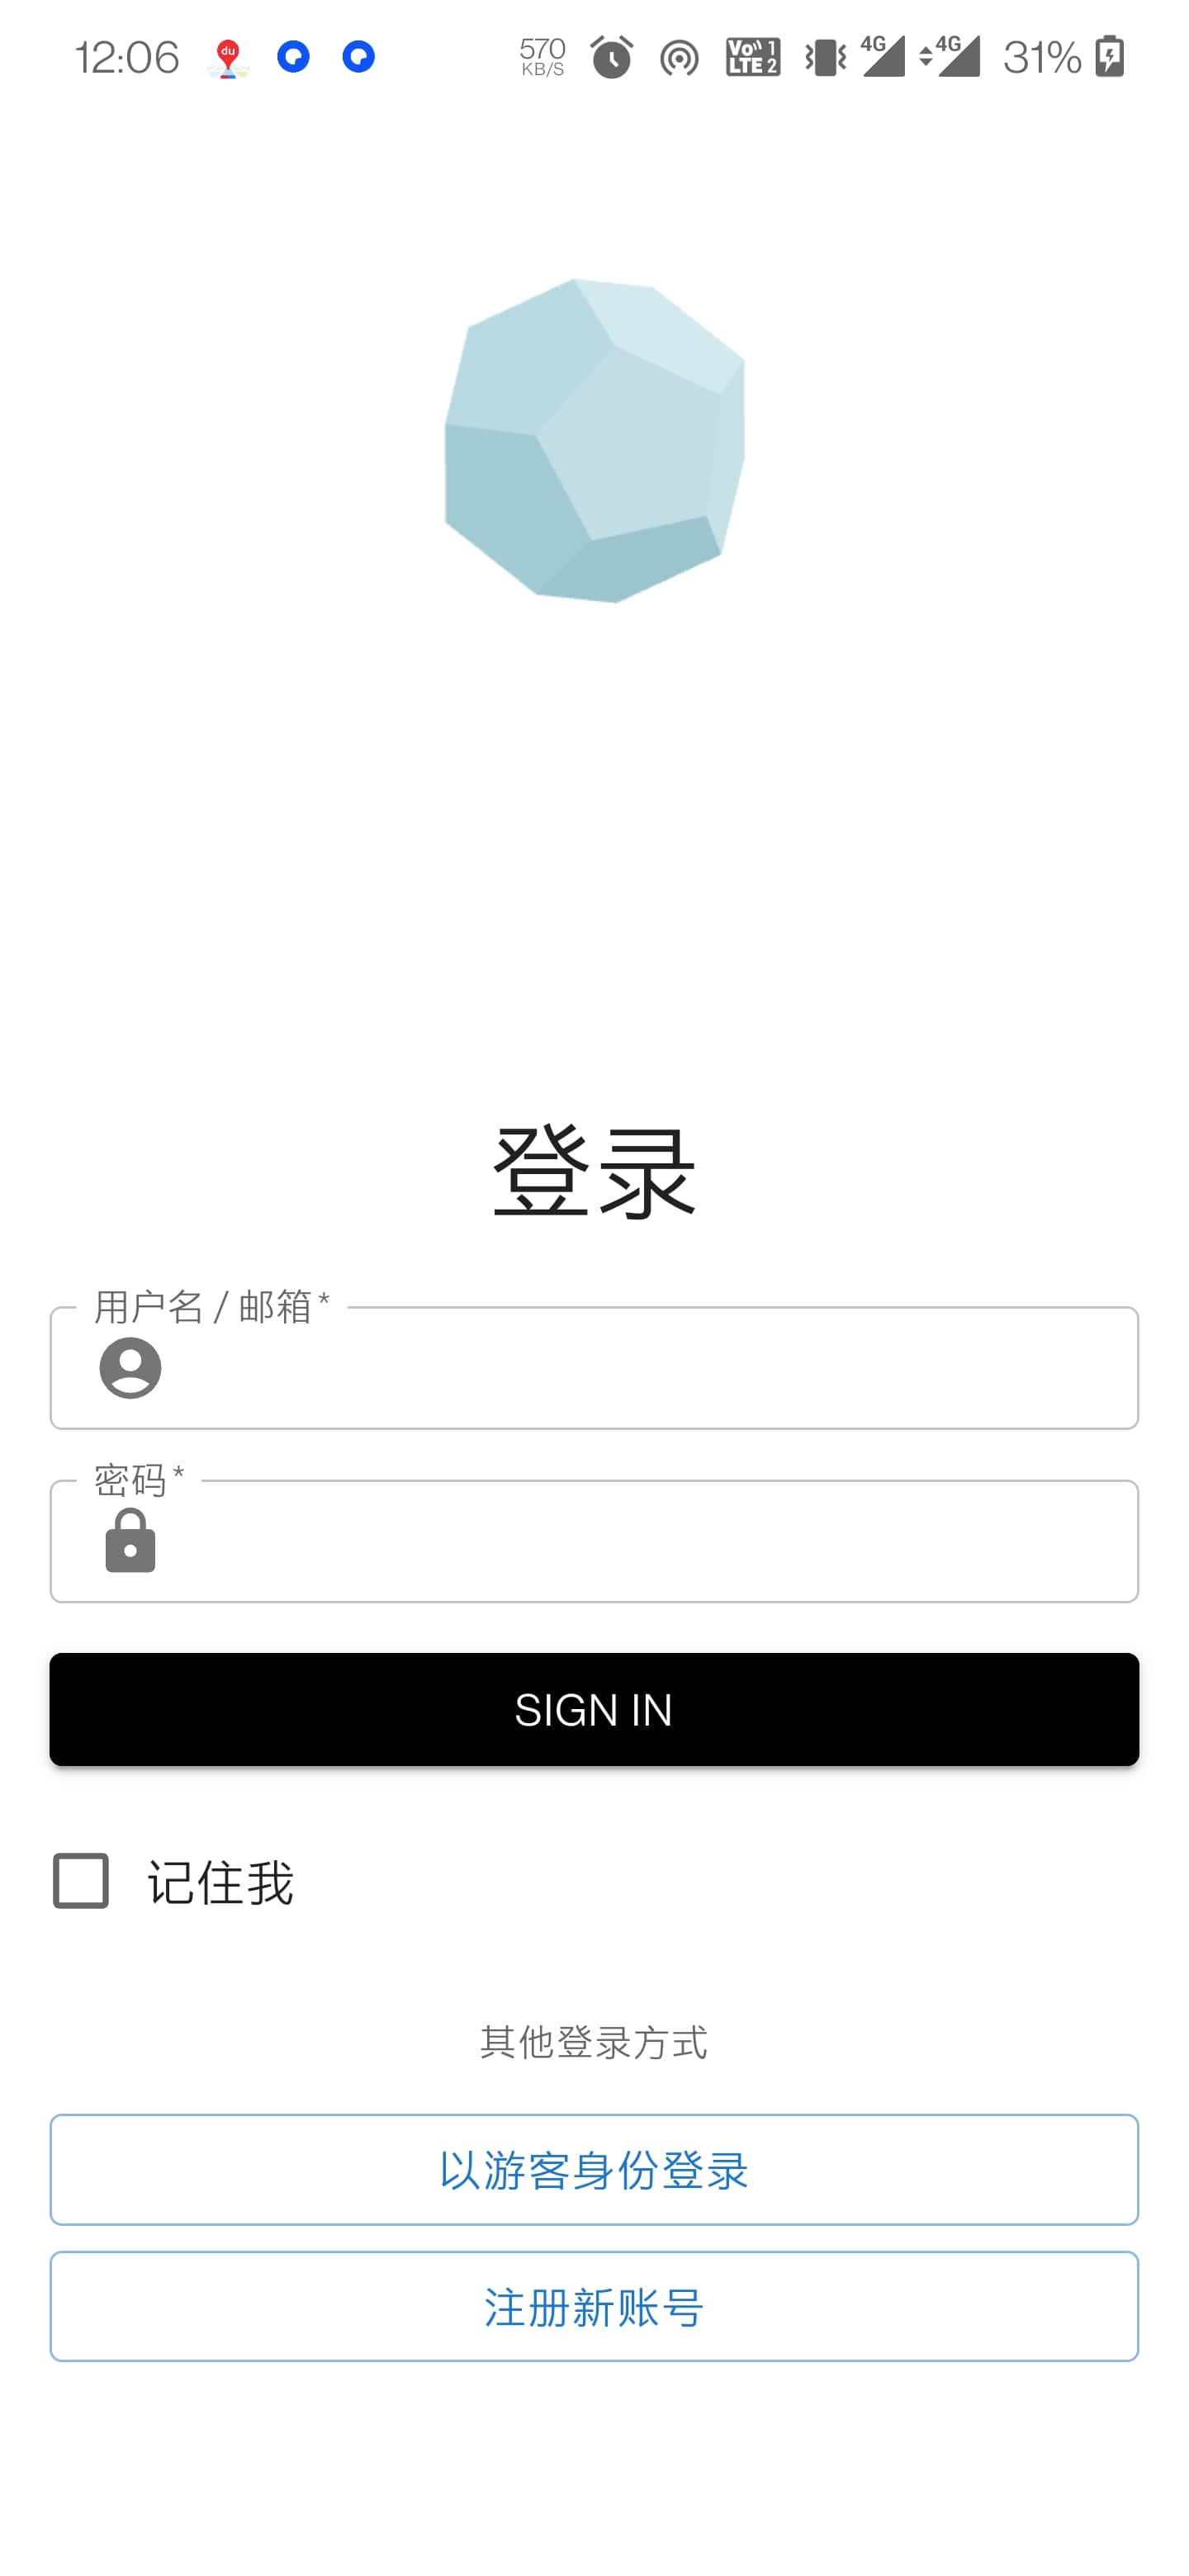
\includegraphics[width=4cm]{./figs/login.jpg}};
      \draw [Circle-] (-1.75,-0.3) -- (-3,-0.3) node [left] {输入用户名或邮箱};
      \draw [Circle-] (-1.75,-0.8) -- (-3,-0.8) node [left] {输入密码};
      \draw [Circle-] (-1.75,-1.5) -- (-3,-1.5) node [left] {点击提交表单};
      \draw [Circle-] (-1.75,-2.1) -- (-3,-2.1) node [left] {localstroge 登录记录};
      \draw [Circle-] (1.75,-2.1) -- (3,-2.1) node [right] {重制密码};
      \draw [Circle-] (-1.75,-2.9) -- (-3,-2.9) node [left] {跳过登录,进入系统};
      \draw [Circle-] (-1.75,-3.3) -- (-3,-3.3) node [left] {进入注册界面};
    \end{scope}
  \end{tikzpicture}
  \caption{登录界面}
  \label{fig:登录界面}
\end{figure}

注册界面提供新用户注册功能,注册逻辑与常用手机 app 相同,必填数据选以 * 标注,注册界面如图\ref{fig:注册界面}所示:

\begin{figure}[H]
  \small
  \centering
  \begin{tikzpicture}[font=\footnotesize]
    \begin{scope}[xshift=0cm]
      \node () at (-7,0) {};
      \node () at (7,0) {};
      \node [draw=black!60] (fig) at (0,0) {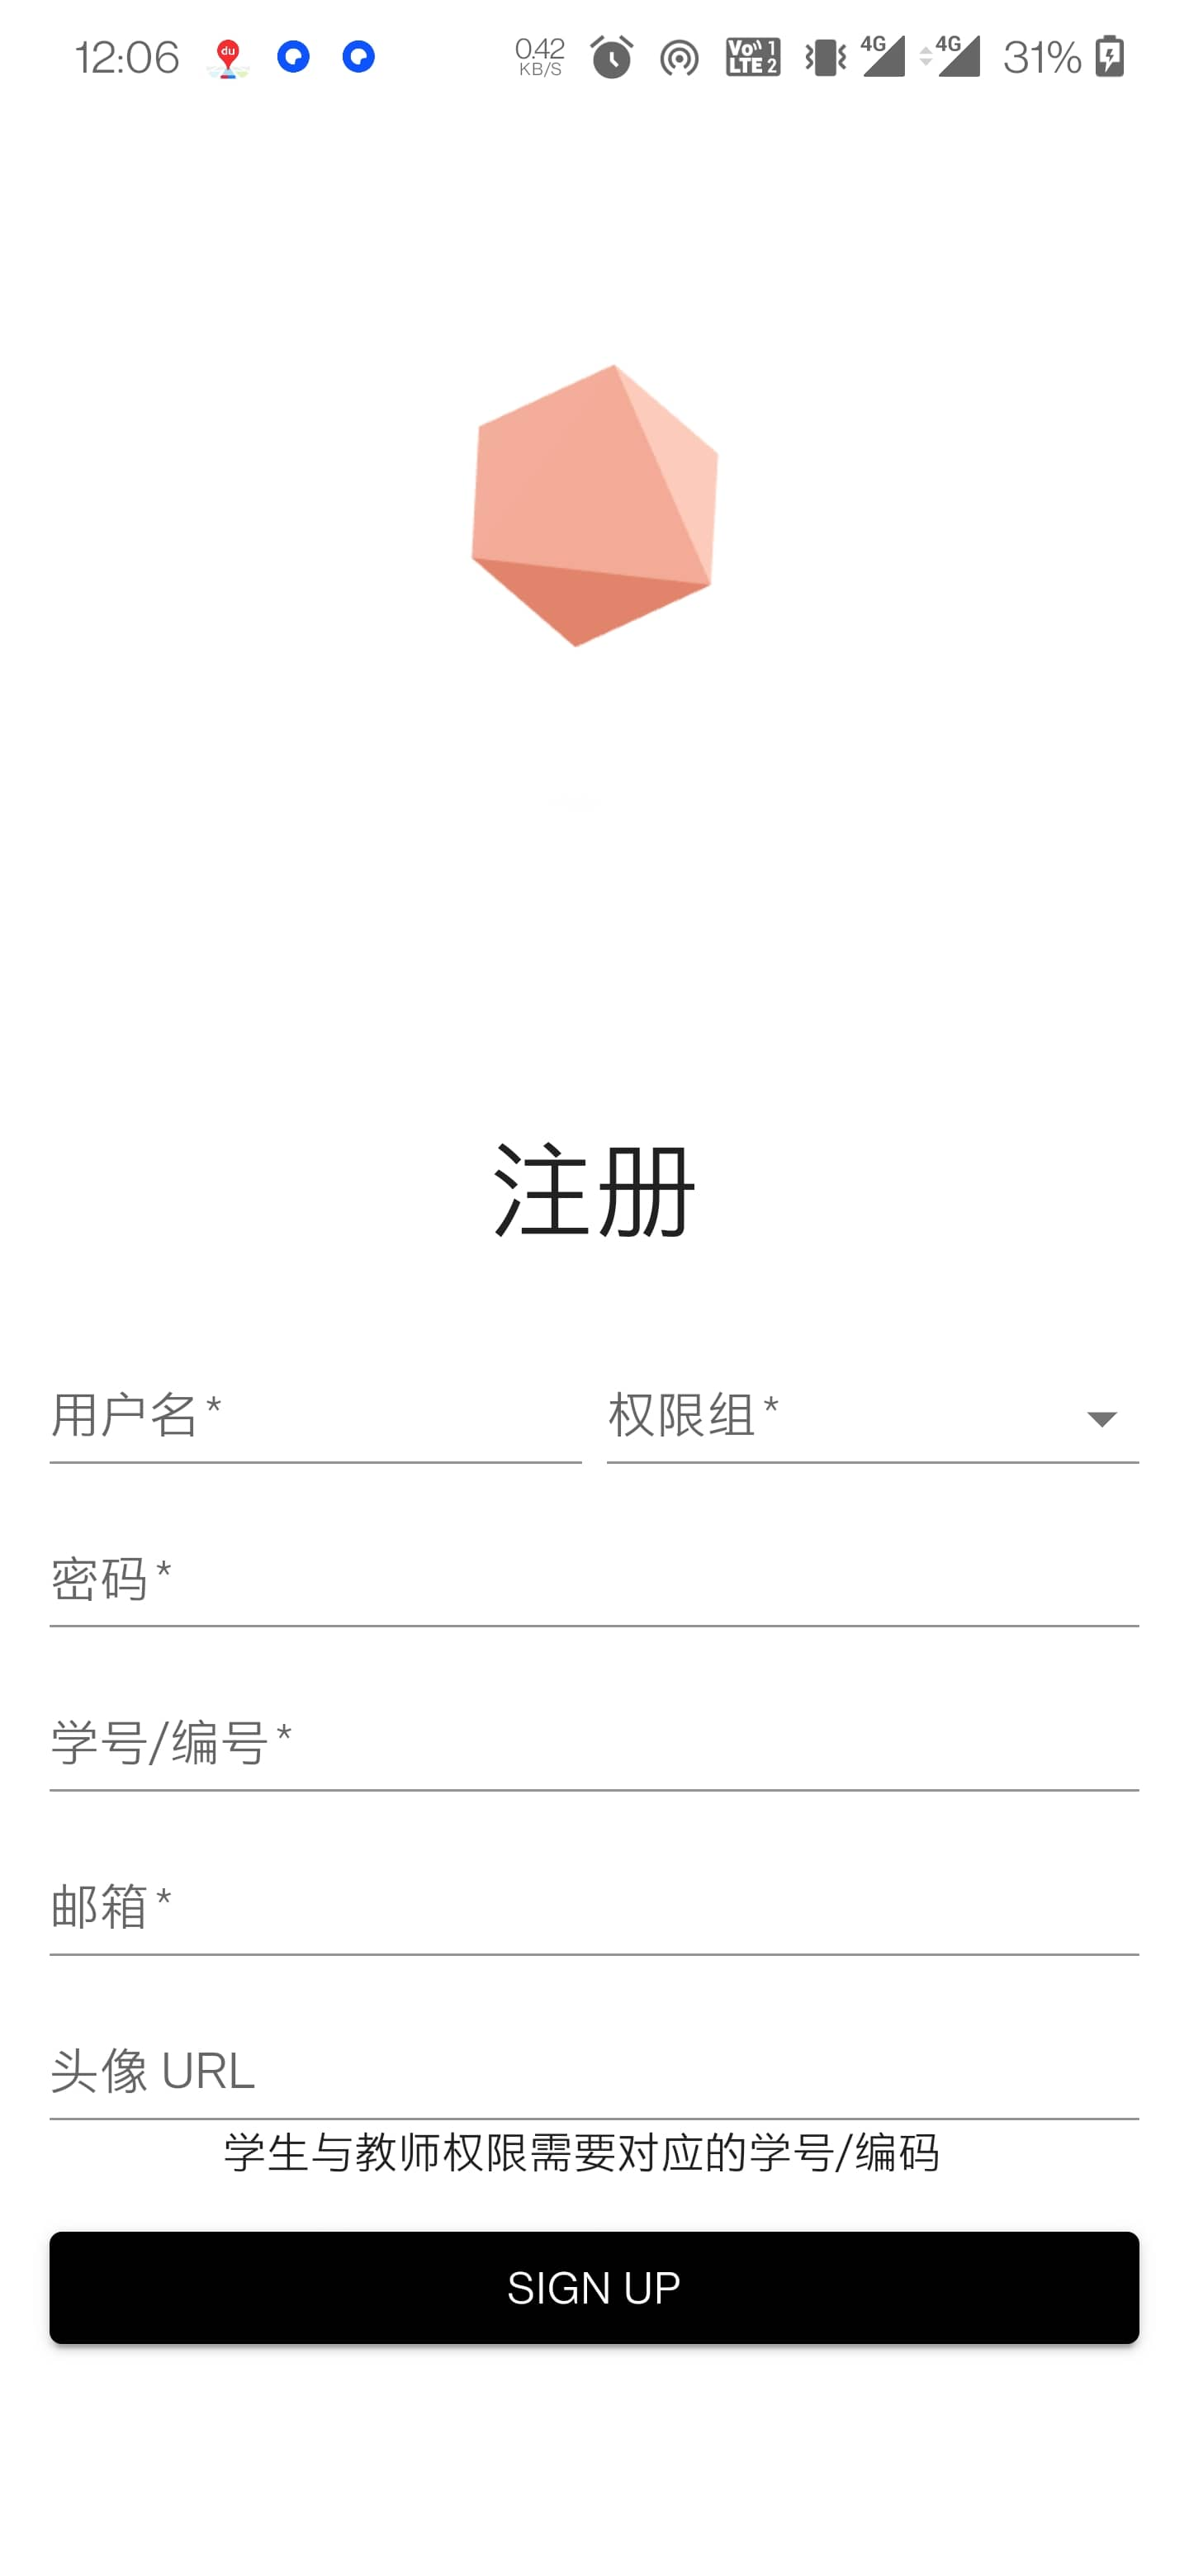
\includegraphics[width=4cm]{./figs/registry.jpg}};
      \draw [Circle-] (-1.75,0) -- (-3,0) node [left] {必填数据段,* 标识};
      \draw [Circle-] (-1.75,-0.9) -- (-3,-0.9) node [left] {可选数据段};
      \draw [Circle-] (-1.75,-2.8) -- (-3,-2.8) node [left] {注册按钮,提交表单};
    \end{scope}
  \end{tikzpicture}
  \caption{注册界面}
  \label{fig:注册界面}
\end{figure}

我的界面向用户展示个人信息,同时提供一些快捷服务,用户可以在此修改个人信息,我的界面如图\ref{fig:我的界面}所示:

\begin{figure}[H]
  \small
  \centering
  \begin{tikzpicture}[font=\footnotesize]
    \begin{scope}[xshift=0cm]
      \node () at (-7,0) {};
      \node () at (7,0) {};
      \node [draw=black!60] (fig) at (0,0) {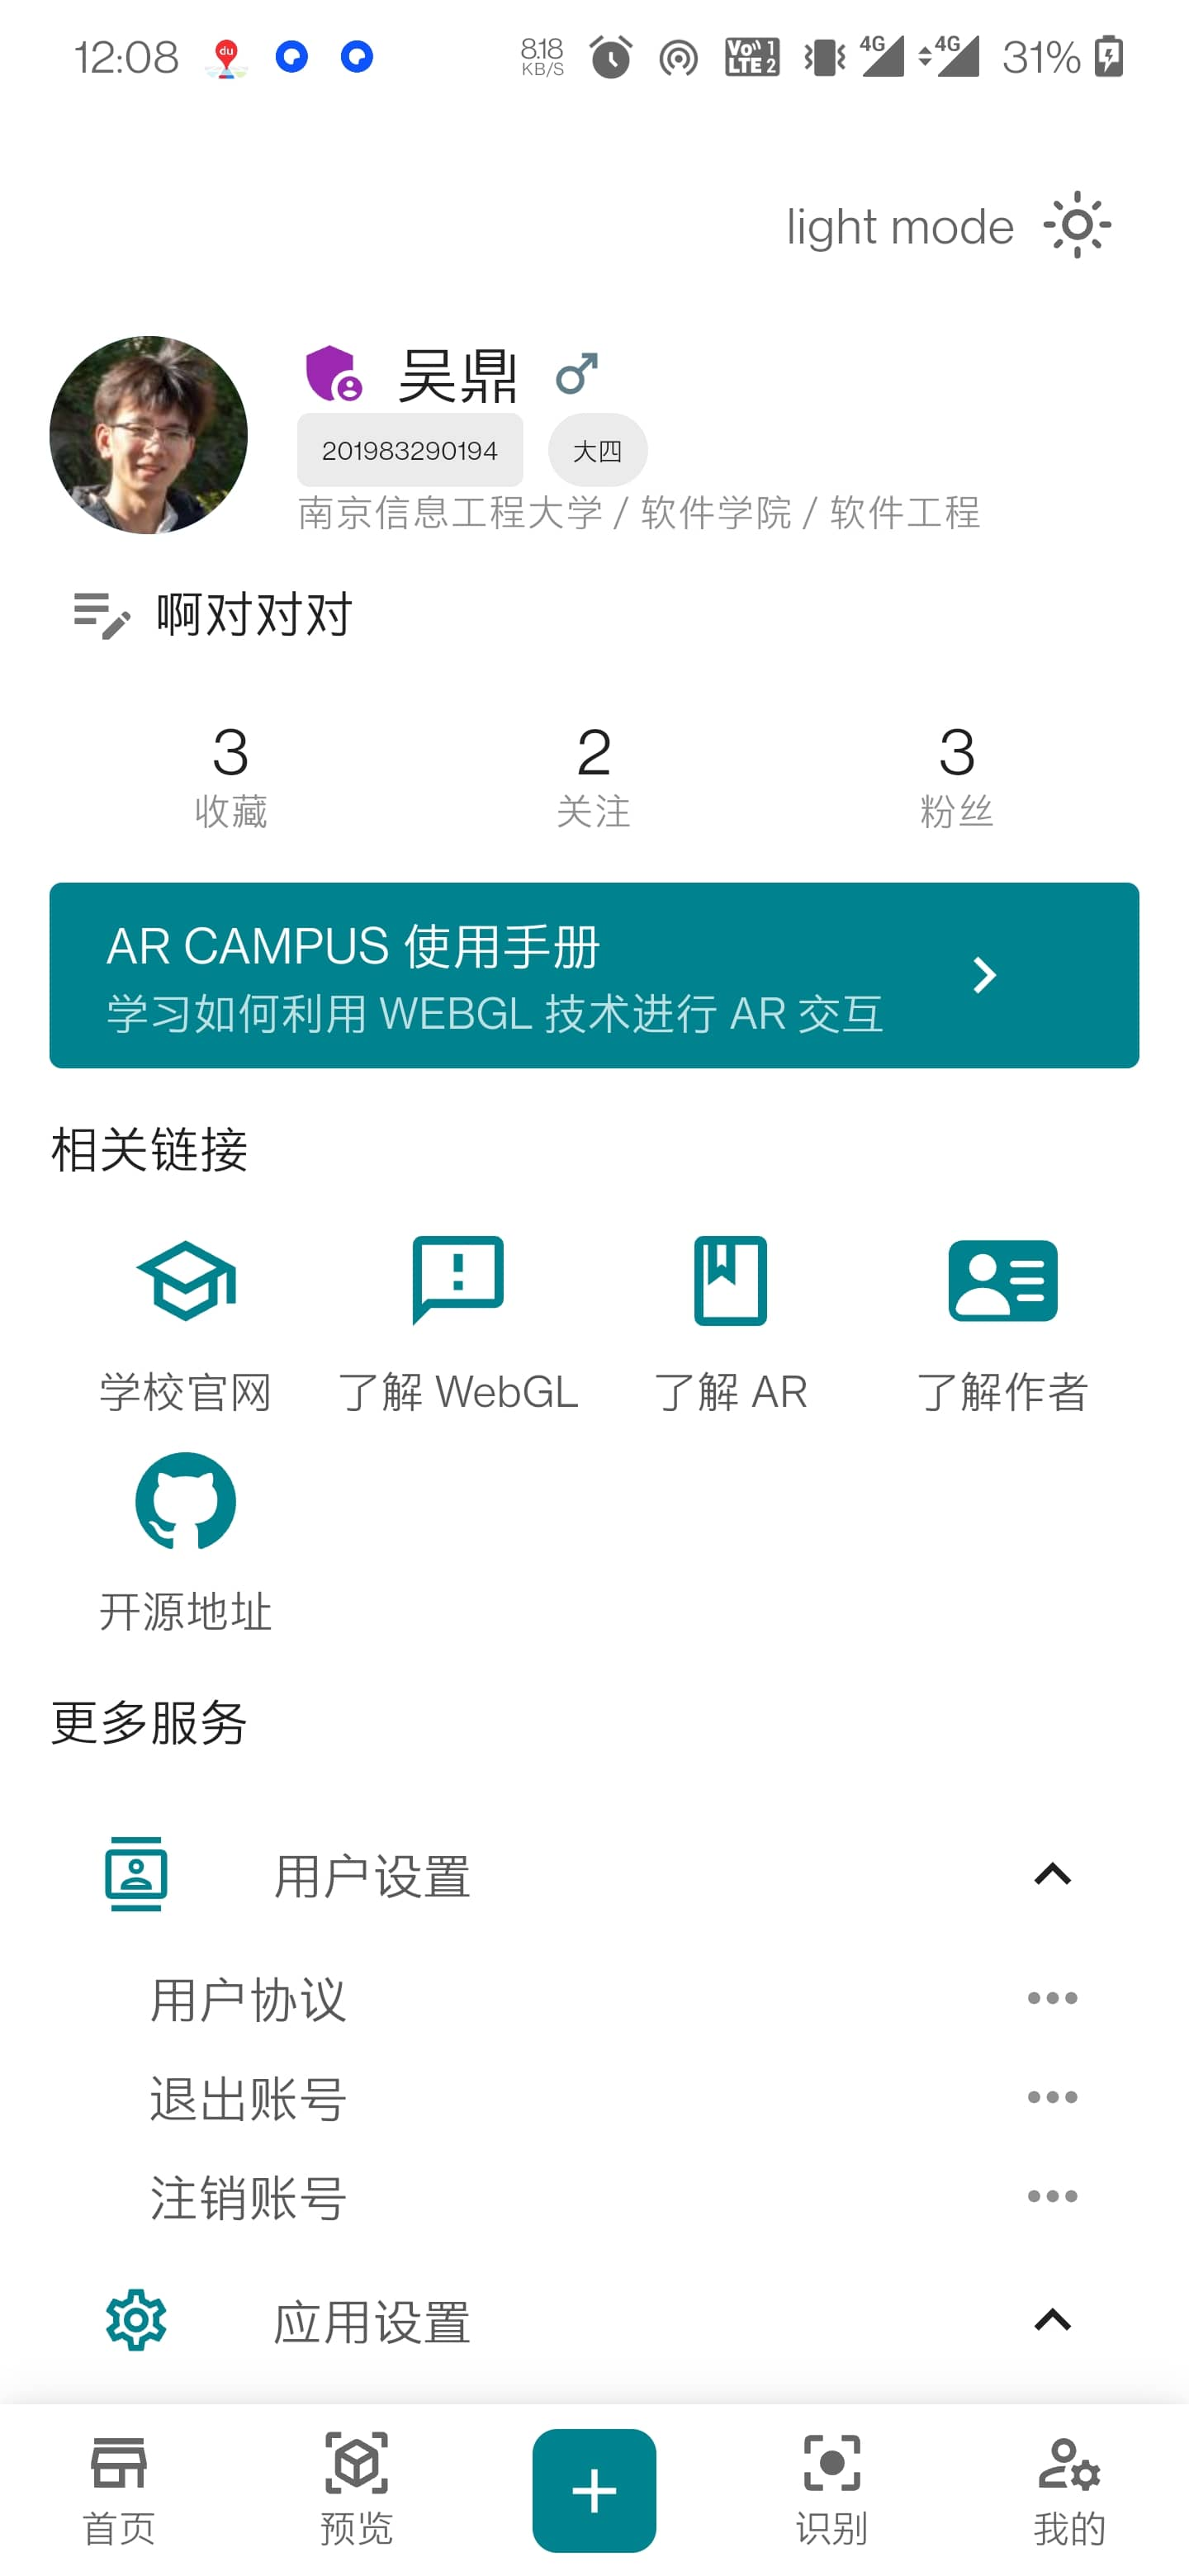
\includegraphics[width=4cm]{./figs/my.jpg}};
      \draw [Circle-] (1.75,3.6) -- (3,3.6) node [right] {切换主题,设置主题色};
      \draw [Circle-] (-1.75,2.88) -- (-3,2.88) node [left] {用户主要信息};
      \draw [Circle-] (-1.75,2.25) -- (-3,2.25) node [left] {修改签名};
      \draw [Circle-] (0.25,1.75) -- (3,1.75) node [right] {社区信息,点击可查看列表};
      \draw [Circle-] (1.75,1) -- (3,1) node [right] {活动面板,展示主要活动或提示};
      \draw [Circle-] (-1.75,0) -- (-3,0) node [left] {一些服务的快捷链接};
      \draw [Circle-] (-1.75,-1.25) -- (-3,-1.25) node [left] {设置,可展开};
      \draw [Circle-] (-1.75,-4) -- (-3,-4) node [left] {其他模块链接};
    \end{scope}
  \end{tikzpicture}
  \caption{我的界面}
  \label{fig:我的界面}
\end{figure}

\subsubsection{数据推送}

数据推送模块包含首页界面。

用户进入首页可根据需求选择分区: ``为你推荐'', ``最新更新'', ``我的关注''。后端将根据用户选择采用对应算法传输可用数据到前端。同时用户也可手动搜索内容。

主页瀑布流中将显示各个模型的简要信息,包括预览图片,名称,作者等,用户点击对应卡片即可预览 3D 模型。``主页''界面如图\ref{fig:主页界面}所示:

\begin{figure}[H]
  \small
  \centering
  \begin{tikzpicture}[font=\footnotesize]
    \begin{scope}[xshift=0cm]
      \node () at (-7,0) {};
      \node () at (7,0) {};
      \node [draw=black!60] (fig) at (0,0) {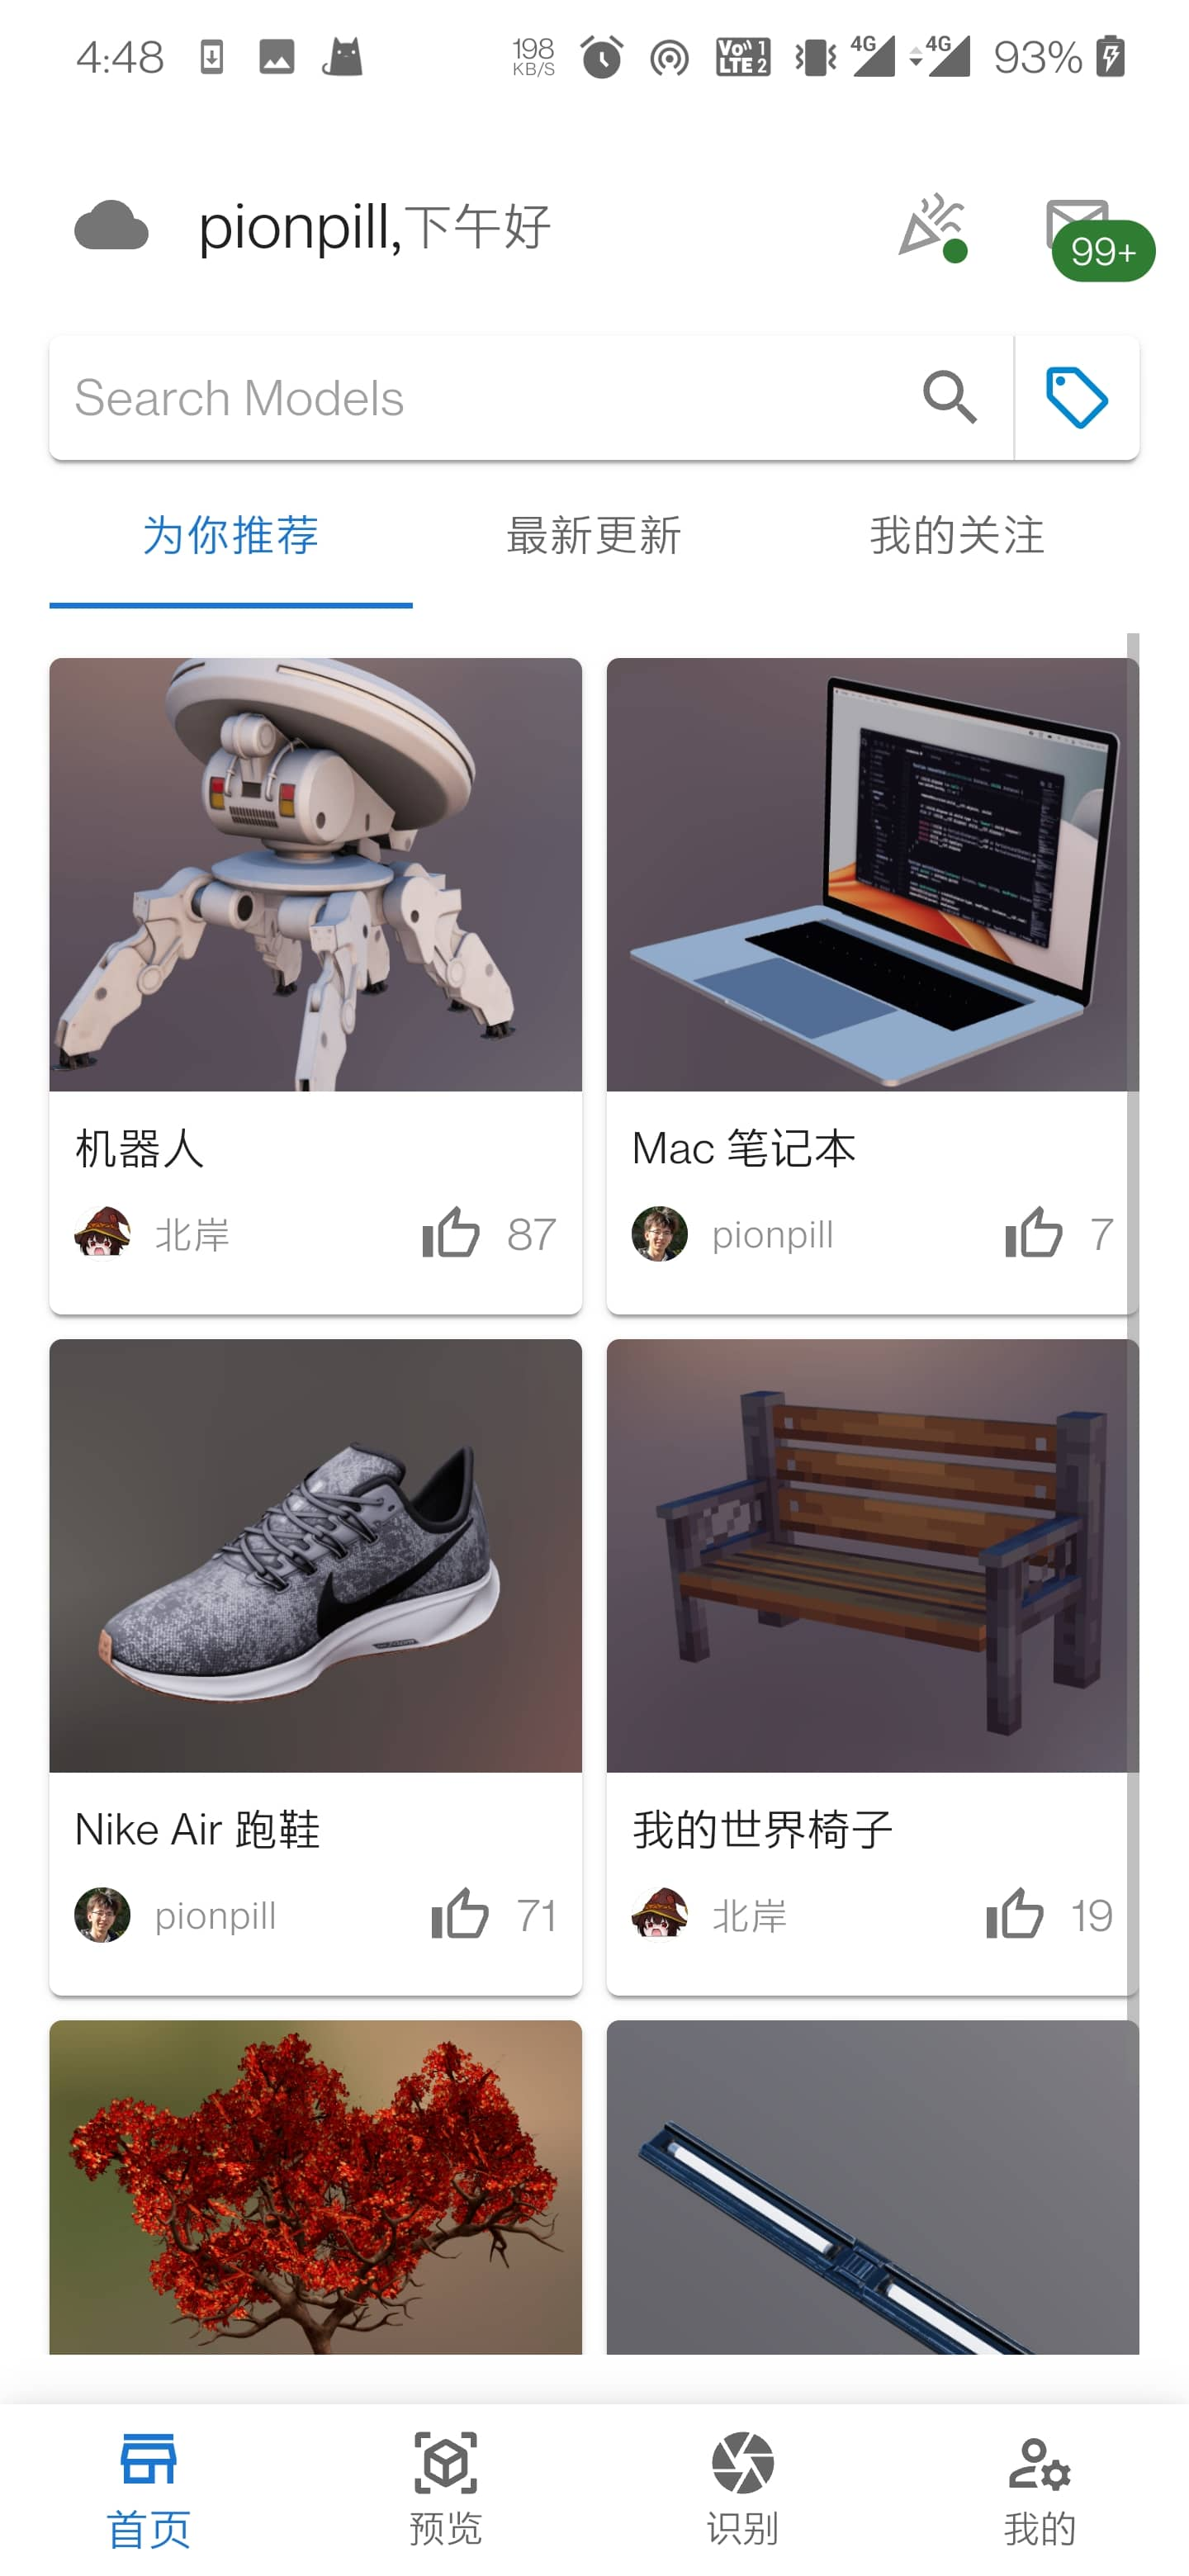
\includegraphics[width=4cm]{./figs/home.jpg}};
      \draw [Circle-] (1.1,3.5) |- (3,3.8) node [right] {系统的一些更新提示};
      \draw [Circle-] (1.75,3.5) -- (3,3.5) node [right] {预留的邮箱功能,可接入邮箱系统};
      \draw [Circle-] (-1.75,3.5) -- (-3,3.5) node [left] {接入高德天气服务};
      \draw [Circle-] (-1.75,2.95) -- (-3,2.95) node [left] {搜索框};
      \draw [Circle-] (-1.75,2.5) -- (-3,2.5) node [left] {分区类型};
      \draw [Circle-] (-0.5,1) -- (-3,1) node [left] {模型卡,点击预览};
      \draw [Circle-] (0.75,1.75) -- (3,1.75) node [right] {模型封面};
      \draw [Circle-] (1,0.5) -- (3,0.5) node [right] {模型名称};
      \draw [Circle-] (-1.75,0.2) -- (-3,0.2) node [left] {作者};
      \draw [Circle-] (1.5,0.2) -- (3,0.2) node [right] {点赞数据};
      \draw [Circle-] (-1.75,-4) -- (-3,-4) node [left] {其他模块链接};
    \end{scope}
  \end{tikzpicture}
  \caption{主页界面}
  \label{fig:主页界面}
\end{figure}

\subsection{核心功能实现}
\subsubsection{WebGL 模块}

WebGL 模块包含模型预览界面。

用户进入模型预览界面后,系统将搭建场景,显示模型信息,请求模型信息数据:
\begin{itemize}
  \item 搭建场景: 系统通过模型 id 查模型表和模型控制表,获取模型 url 和相关配置信息。此时系统将显示场景。
  \item 请求模型: 系统获取模型 url 后异步请求模型数据,继而在界面上显示。
  \item 模型信息: 系统向后端请求模型的文本,点赞,作者等信息。
\end{itemize}

其中搭建场景,显示模型信息的功能同步进行,模型数据异步请求。

预览界面将模型信息分为简要信息与详细信息,简要信息仅以浮动卡片形式显现,用户可隐藏相关信息。详细信息则无法隐藏。用户在移动设备上可通过触摸移动位置,双指缩放模型大小,也可以通过控制板调整环境信息,例如背景贴图,背景模糊程度。模型预览界面如图\ref{fig:模型预览界面}所示:

\begin{figure}[H]
  \small
  \centering
  \begin{tikzpicture}[font=\footnotesize]
    \node () at (-7,0) {};
    \node () at (7,0) {};
    \begin{scope}[xshift=-2.25cm]
      \node [draw=black!60] (fig) at (0,0) {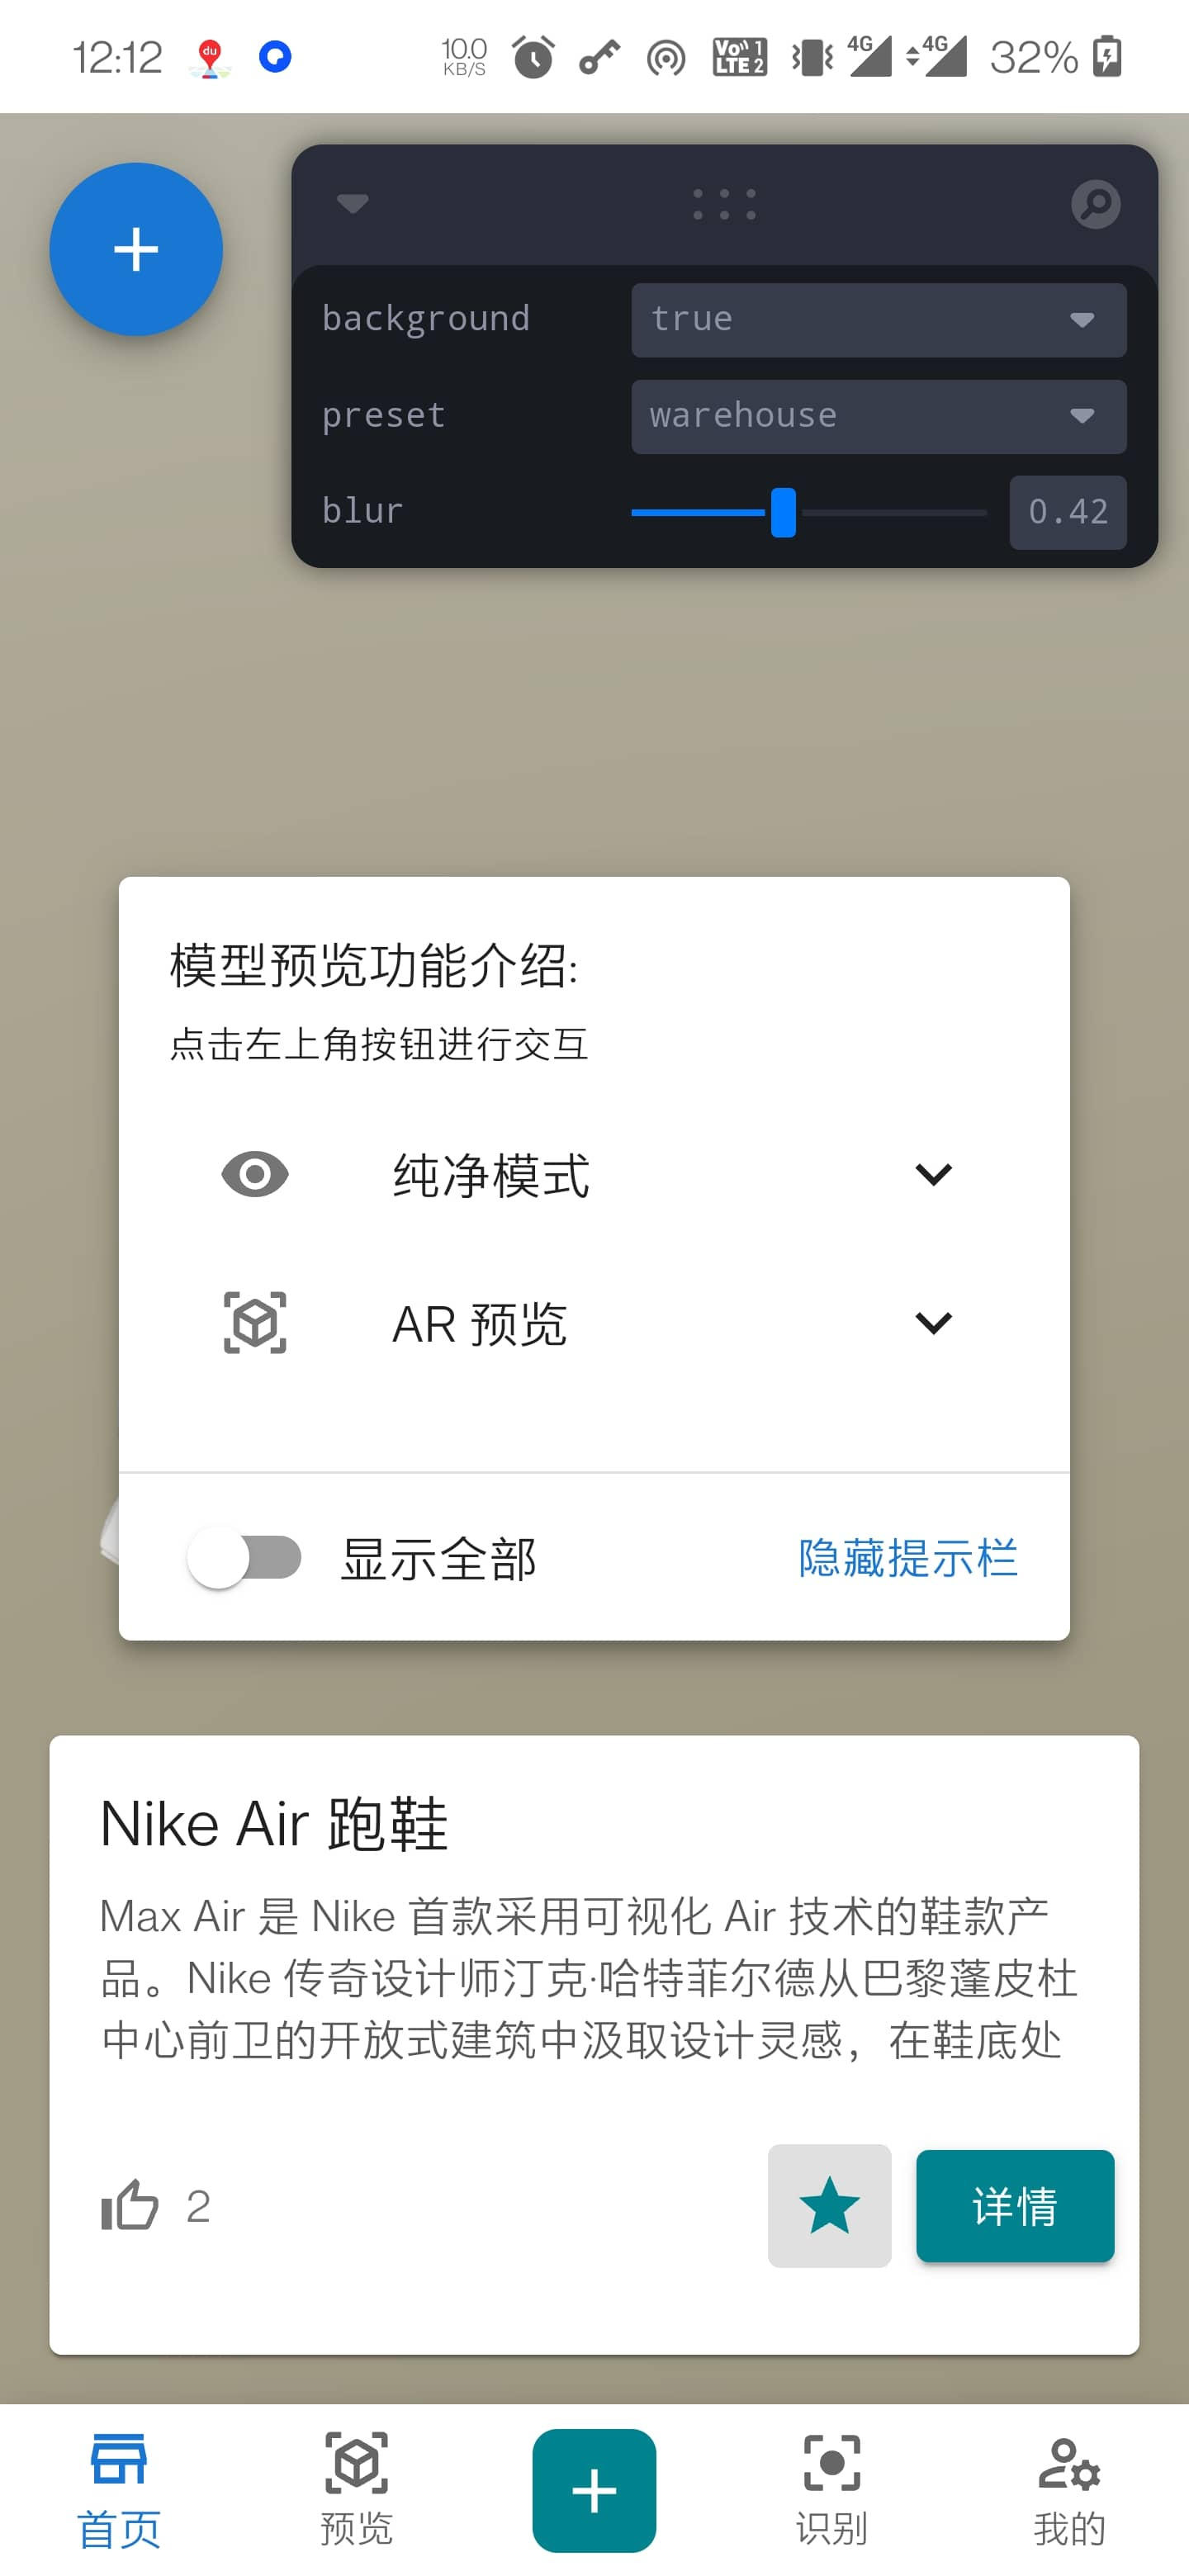
\includegraphics[width=4cm]{./figs/preview.jpg}};
      \draw [Circle-] (-0.5,3.75) -- (-3,3.75) node [left] {控制板};
      \draw [Circle-] (-1.75,3.5) -- (-3,3.5) node [left] {扩展功能按钮};
      \draw [Circle-] (-1.75,2.5) -- (-3,2.5) node [left] {场景背景};
      \draw [Circle-] (-1.5,0.2) -- (-3,0.2) node [left] {操作说明};
      \draw [Circle-] (-1.5,-1) -- (-3,-1) node [left] {快捷功能按钮};
      \draw [Circle-] (-1.75,-1.8) -- (-3,-1.8) node [left] {模型名称};
      \draw [Circle-] (-1.75,-2.2) -- (-3,-2.2) node [left] {模型简介};
      \draw [Circle-] (-1,-2.5) -- (-3,-2.5) node [left] {简要信息卡};
      \draw [Circle-] (-1.75,-3.1) -- (-3,-3.1) node [left] {模型点赞数据};
      \draw [Circle-] (0.75,-3.1) |- (-3,-2.8) node [left] {用户收藏按钮};
      \draw [Circle-] (1.5,-3.1) |- (-3,-3.4) node [left] {切换到详细信息};
      \draw [Circle-] (-1.75,-4) -- (-3,-4) node [left] {其他模块链接};
    \end{scope}
    \begin{scope}[xshift=2.25cm]
      \node () at (-7,0) {};
      \node () at (7,0) {};
      \node [draw=black!60] (fig) at (0,0) {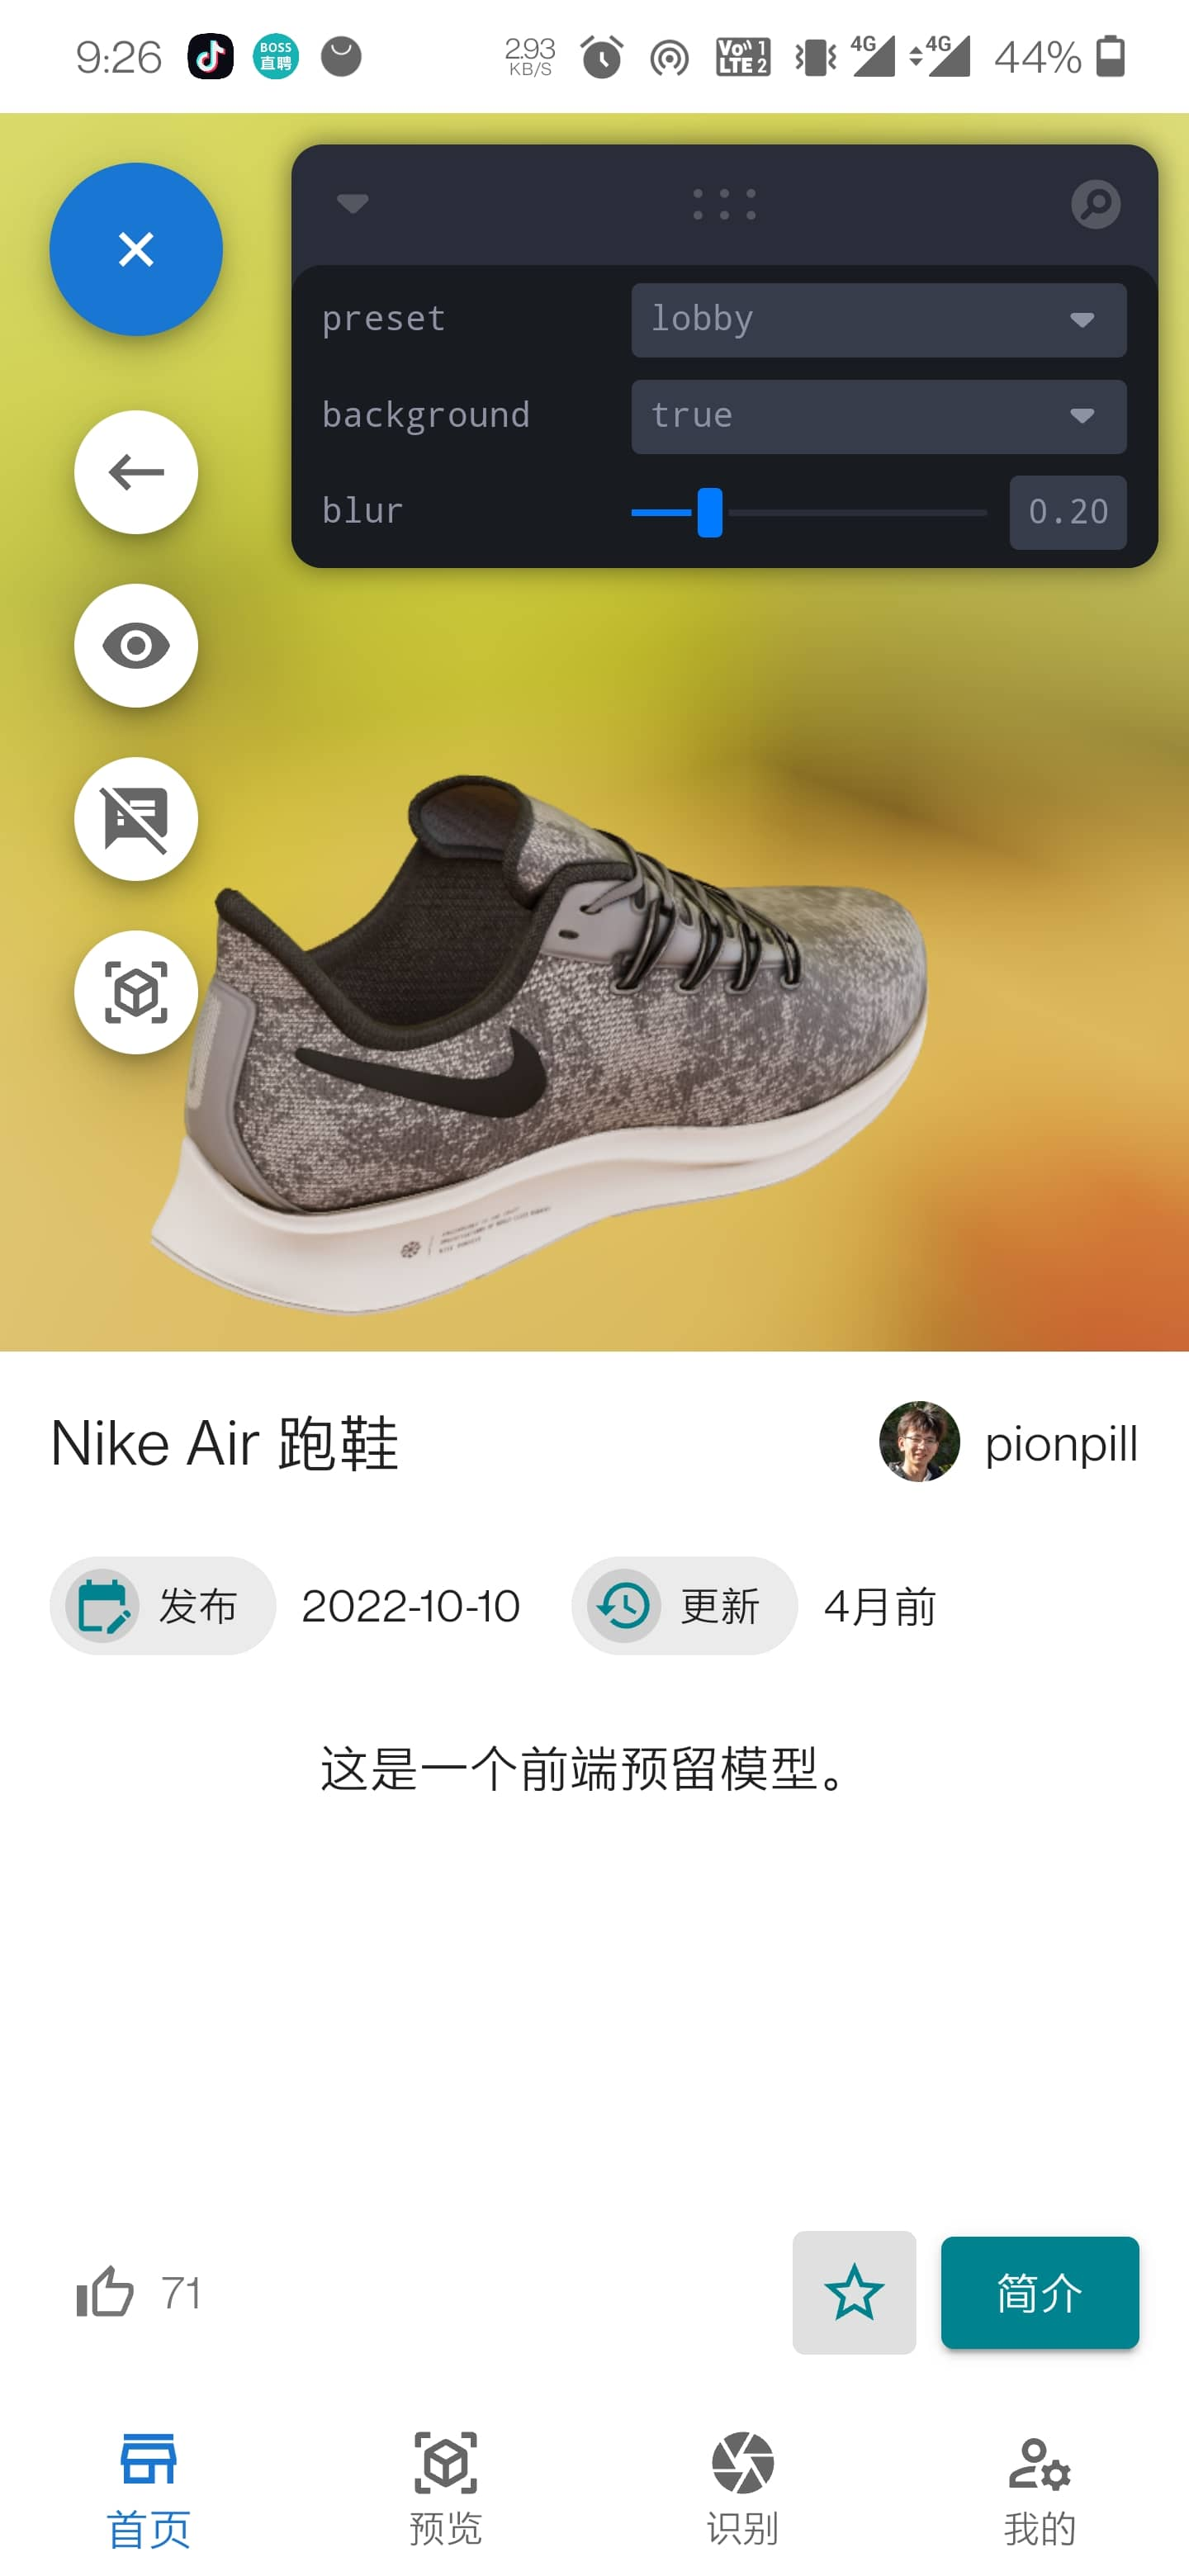
\includegraphics[width=4cm]{./figs/preview-2.jpg}};
      \draw [Circle-] (1.75,3.3) -- (3,3.3) node [right] {切换环境背景};
      \draw [Circle-] (1.75,2.9) -- (3,2.9) node [right] {切换是否显示背景};
      \draw [Circle-] (1.75,2.5) -- (3,2.5) node [right] {设置背景模糊程度};
      \draw [Circle-] (0,0.5) -- (3,0.5) node [right] {模型本体};
      \draw [Circle-] (2,-0.5) -- (3,-0.5) node [right] {作者信息};
      \draw [Circle-] (1.5,-1) -- (3,-1) node [right] {模型发布与更新信息};
      \draw [Circle-] (1.75,-1.8) -- (3,-1.8) node [right] {模型详细信息};
      \draw [Circle-] (1.75,-4) -- (3,-4) node [right] {其他模块链接};
      \draw [Circle-] (-1.4,2.2) -- (3,2.2) node [right] {开关非必要组件};
      \draw [Circle-] (-1.4,1.6) -- (3,1.6) node [right] {开关操作说明};
      \draw [Circle-] (-1.4,1) -- (3,1) node [right] {在 AR 模式中显示};
    \end{scope}
  \end{tikzpicture}
  \caption{模型预览界面}
  \label{fig:模型预览界面}
\end{figure}

\subsubsection{AR 模块}

AR 模块包括 AR 预览与 AR 识别界面。

进入 AR 模式将提醒用户需要的设备条件,如果用户的设备不满足任意条件,AR 按钮将显示 AR unsupported。设备需要满足的条件如下:
\begin{itemize}
  \item 摄像头: 浏览器需要获取摄像头权限, 确保访问的是 https 协议网站,或者手动调整浏览器信任对应网站。否则浏览器无法获得摄像头权限。
  \item AR 服务: 安卓智能机需开启 AR 服务,请在 google play 安装 “面向 AR 的Google Play 服务” 插件。苹果设备开启 ARKit 服务。
  \item 浏览器: 尽量使用 chrome 浏览器,AR 功能至少需要 chrome 80+ 版本。安卓设备尽量保持在系统 11+ 版本。
  \item 网络环境: 出于优化考虑,系统不会一次推送所有数据,AR 部分功能需要实时获取网络资源。
\end{itemize}

AR 提示界面如图\ref{fig:AR提示界面}所示:

\begin{figure}[H]
  \small
  \centering
  \begin{tikzpicture}[font=\footnotesize]
    \begin{scope}[xshift=0cm]
      \node () at (-7,0) {};
      \node () at (7,0) {};
      \node [draw=black!60] (fig) at (0,0) {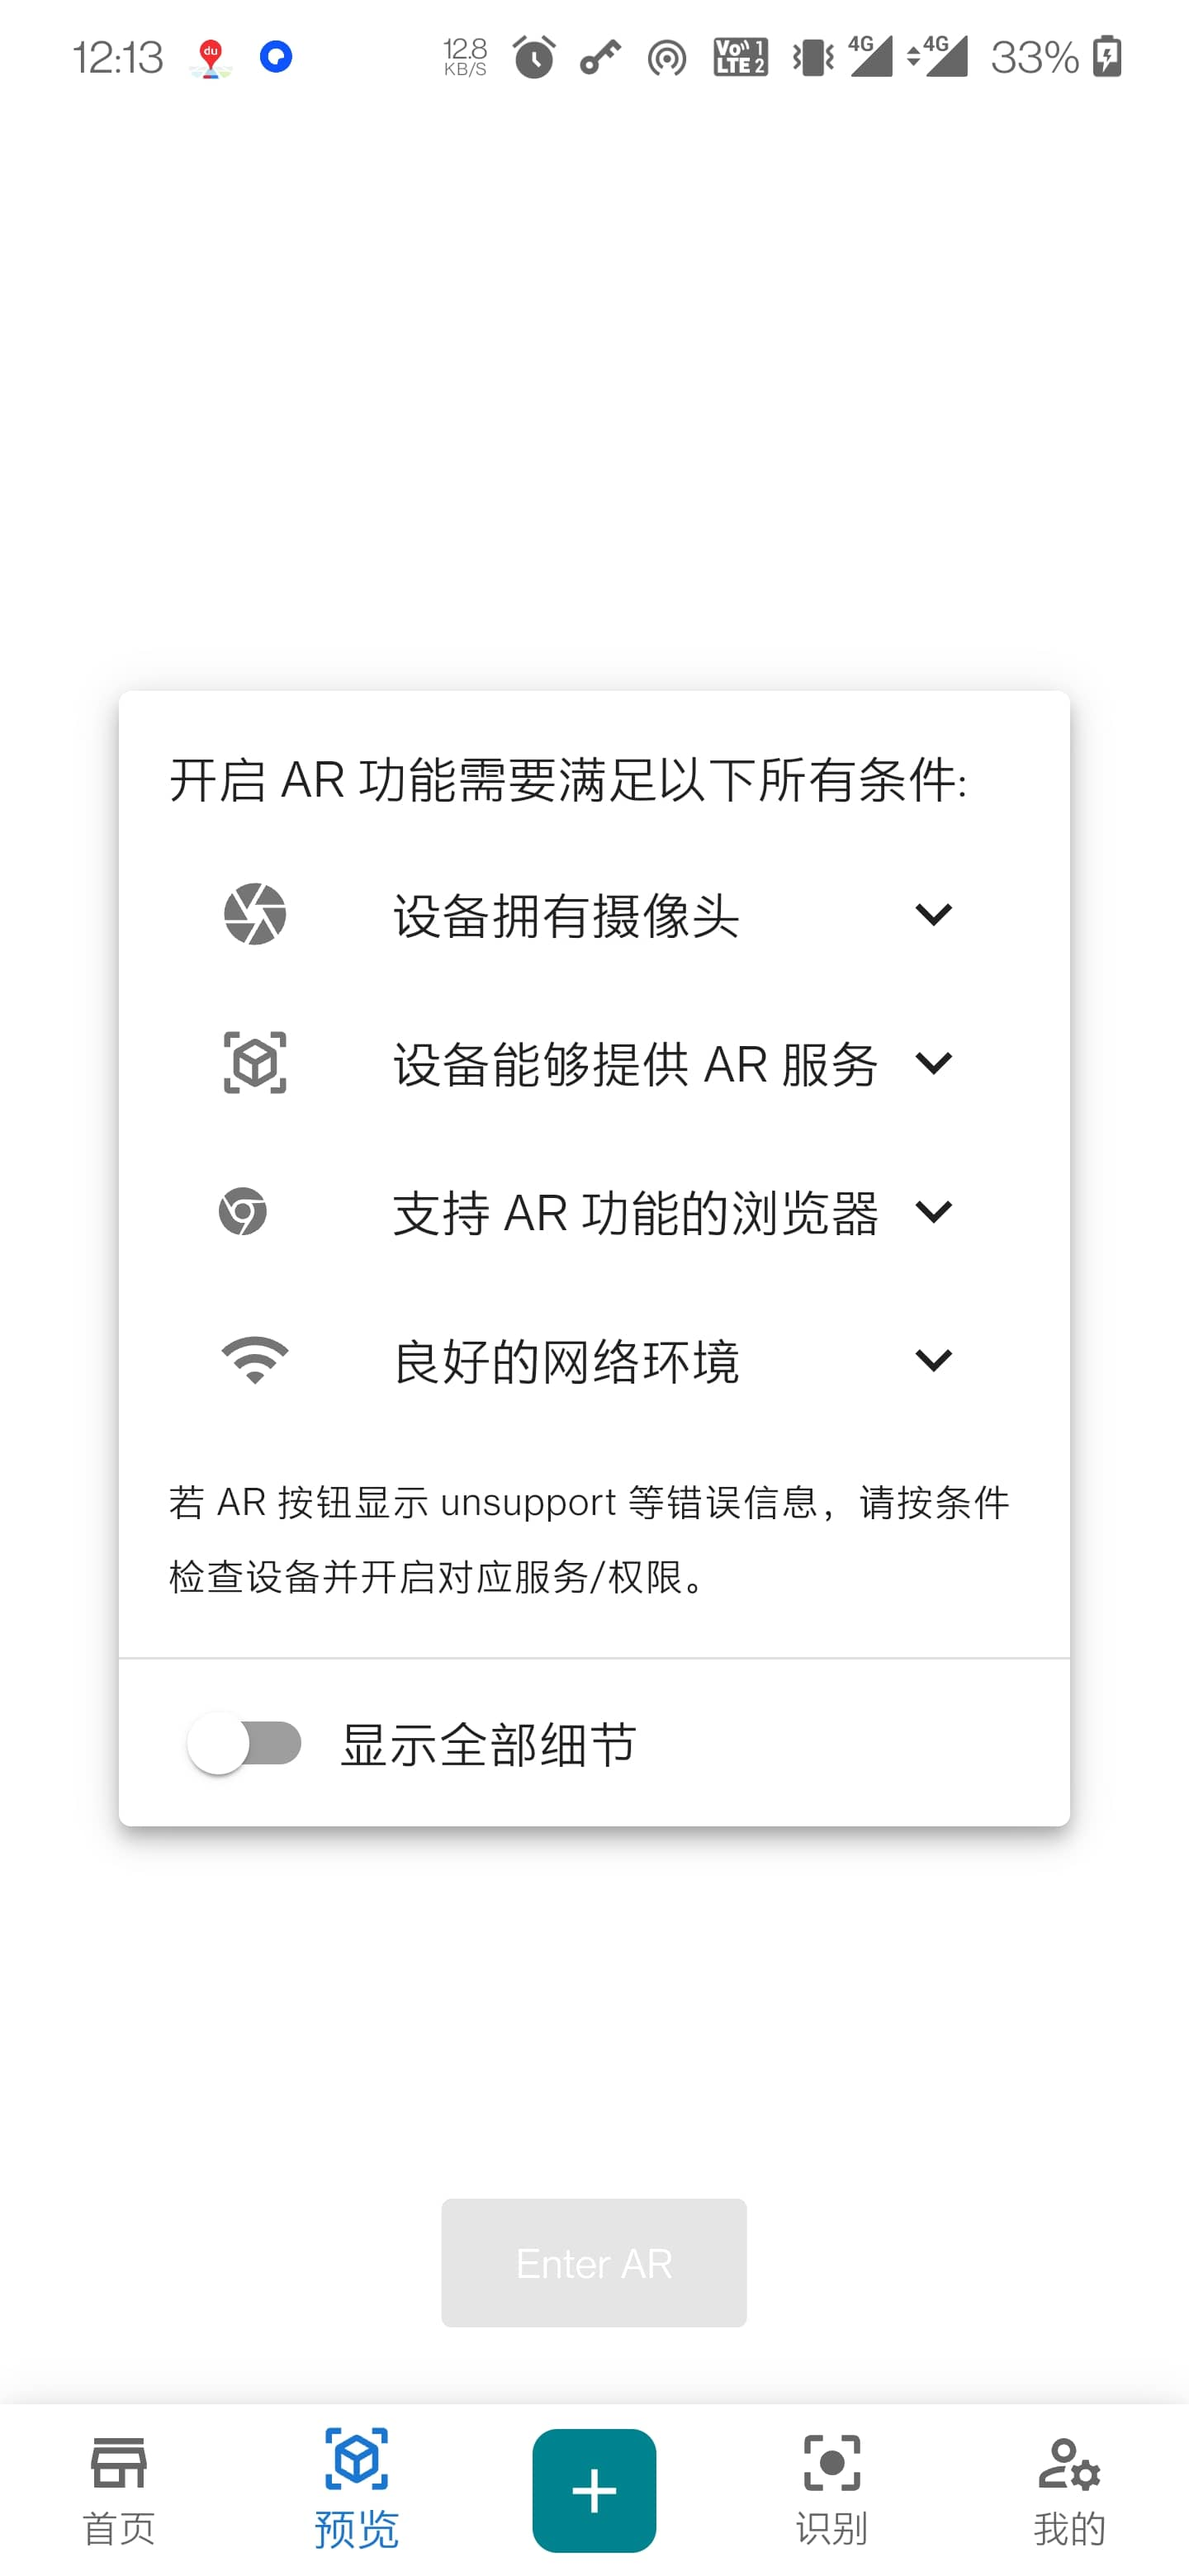
\includegraphics[width=4cm]{./figs/ar.jpg}};
      \draw [Circle-] (-0.5,1) -- (-3,1) node [left] {AR 提示信息};
      \draw [Circle-] (-1.5,-1.5) -- (-3,-1.5) node [left] {快捷操作按钮};
      \draw [Circle-] (-0.5,-3.25) -- (-3,-3.25) node [left] {AR 按钮};
      \draw [Circle-] (-1.75,-4) -- (-3,-4) node [left] {其他模块链接};
    \end{scope}
  \end{tikzpicture}
  \caption{AR提示界面}
  \label{fig:AR提示界面}
\end{figure}

进入 AR 预览界面后,系统会请求手机摄像头权限,用户确认之后,系统将实时获取显示影像,并将 3D 模式显示在界面中,用户可以通过控制板或手动调整操作模型。系统将实时计算模型所在位置,AR 预览界面如图\ref{fig:AR预览界面}所示:

\begin{figure}[H]
  \small
  \centering
  \begin{tikzpicture}[font=\footnotesize]
    \node () at (-7,0) {};
    \node () at (7,0) {};
    \begin{scope}[xshift=-2.25cm]
      \node [draw=black!60] (fig) at (0,0) {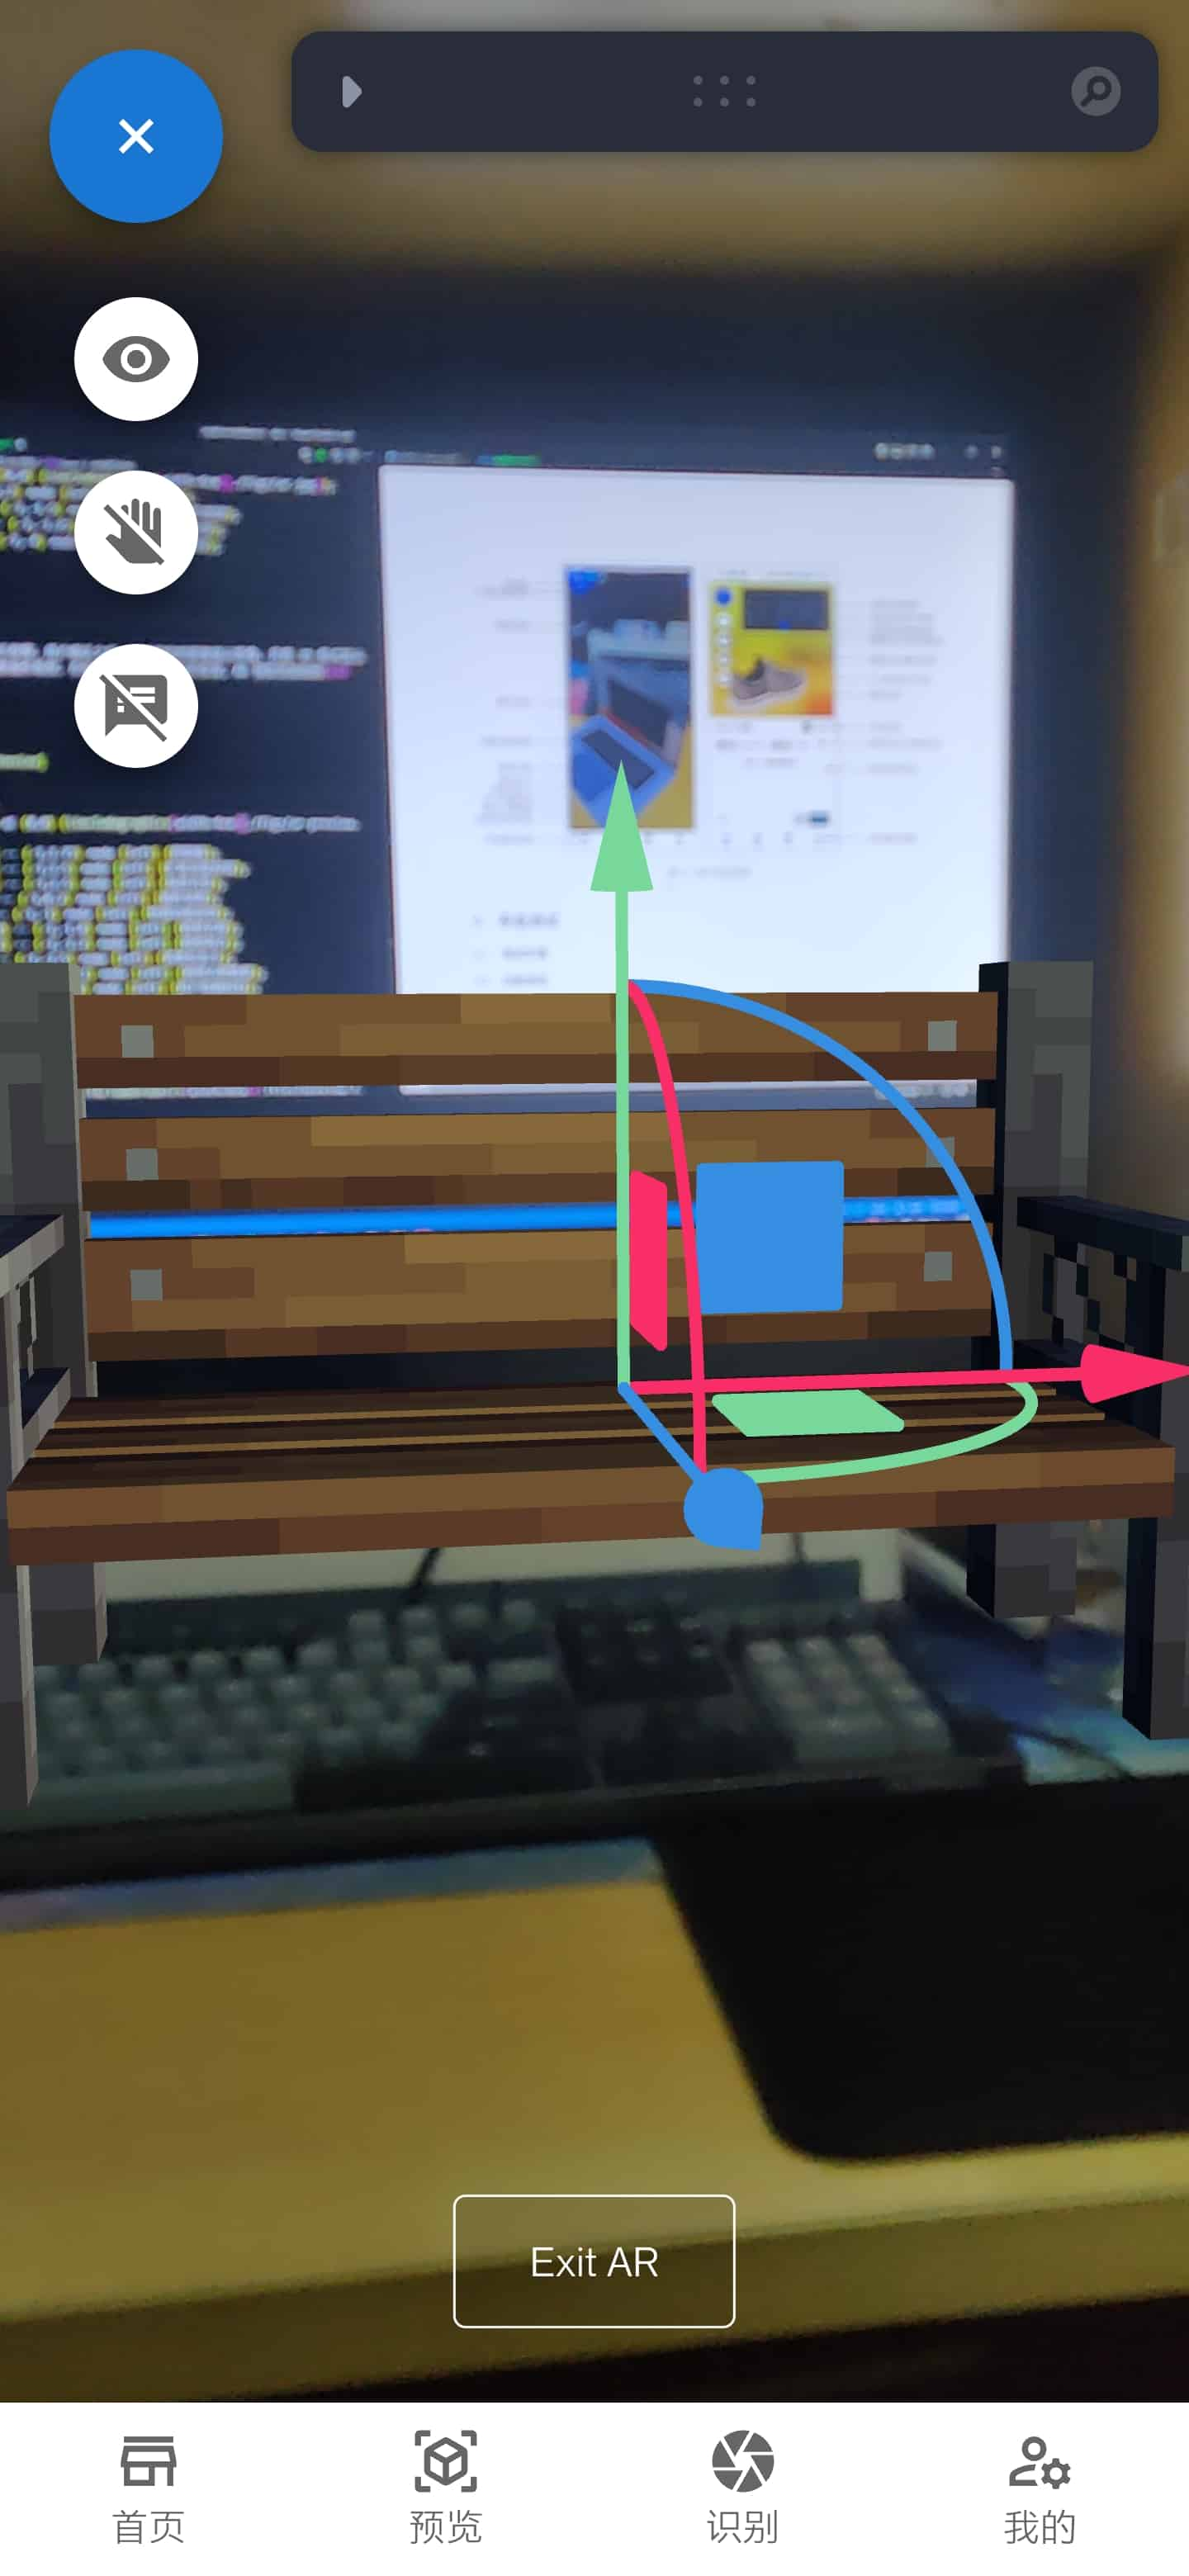
\includegraphics[width=4cm]{./figs/ar-preview.jpg}};
      \draw [Circle-] (-0.5,4) -- (-3,4) node [left] {控制板};
      \draw [Circle-] (-1.75,3.75) -- (-3,3.75) node [left] {扩展功能按钮};
      \draw [Circle-] (-1.75,3.1) -- (-3,3.1) node [left] {开关非必要组件};
      \draw [Circle-] (-1.75,2.5) -- (-3,2.5) node [left] {允许/禁止触控};
      \draw [Circle-] (-1.75,1.9) -- (-3,1.9) node [left] {开关操作说明};
      \draw [Circle-] (-1.5,0) -- (-3,0) node [left] {模型本体};
      \draw [Circle-] (0.5,-0.5) -- (-3,-0.5) node [left] {触摸操作轴};
      \draw [Circle-] (-1.5,-2) -- (-3,-2) node [left] {现实场景};
      \draw [Circle-] (-0.25,-3.25) -- (-3,-3.25) node [left] {AR 按钮};
      \draw [Circle-] (-1.75,-4) -- (-3,-4) node [left] {其他模块链接};
    \end{scope}
    \begin{scope}[xshift=2.25cm]
      \node [draw=black!60] (fig) at (0,0) {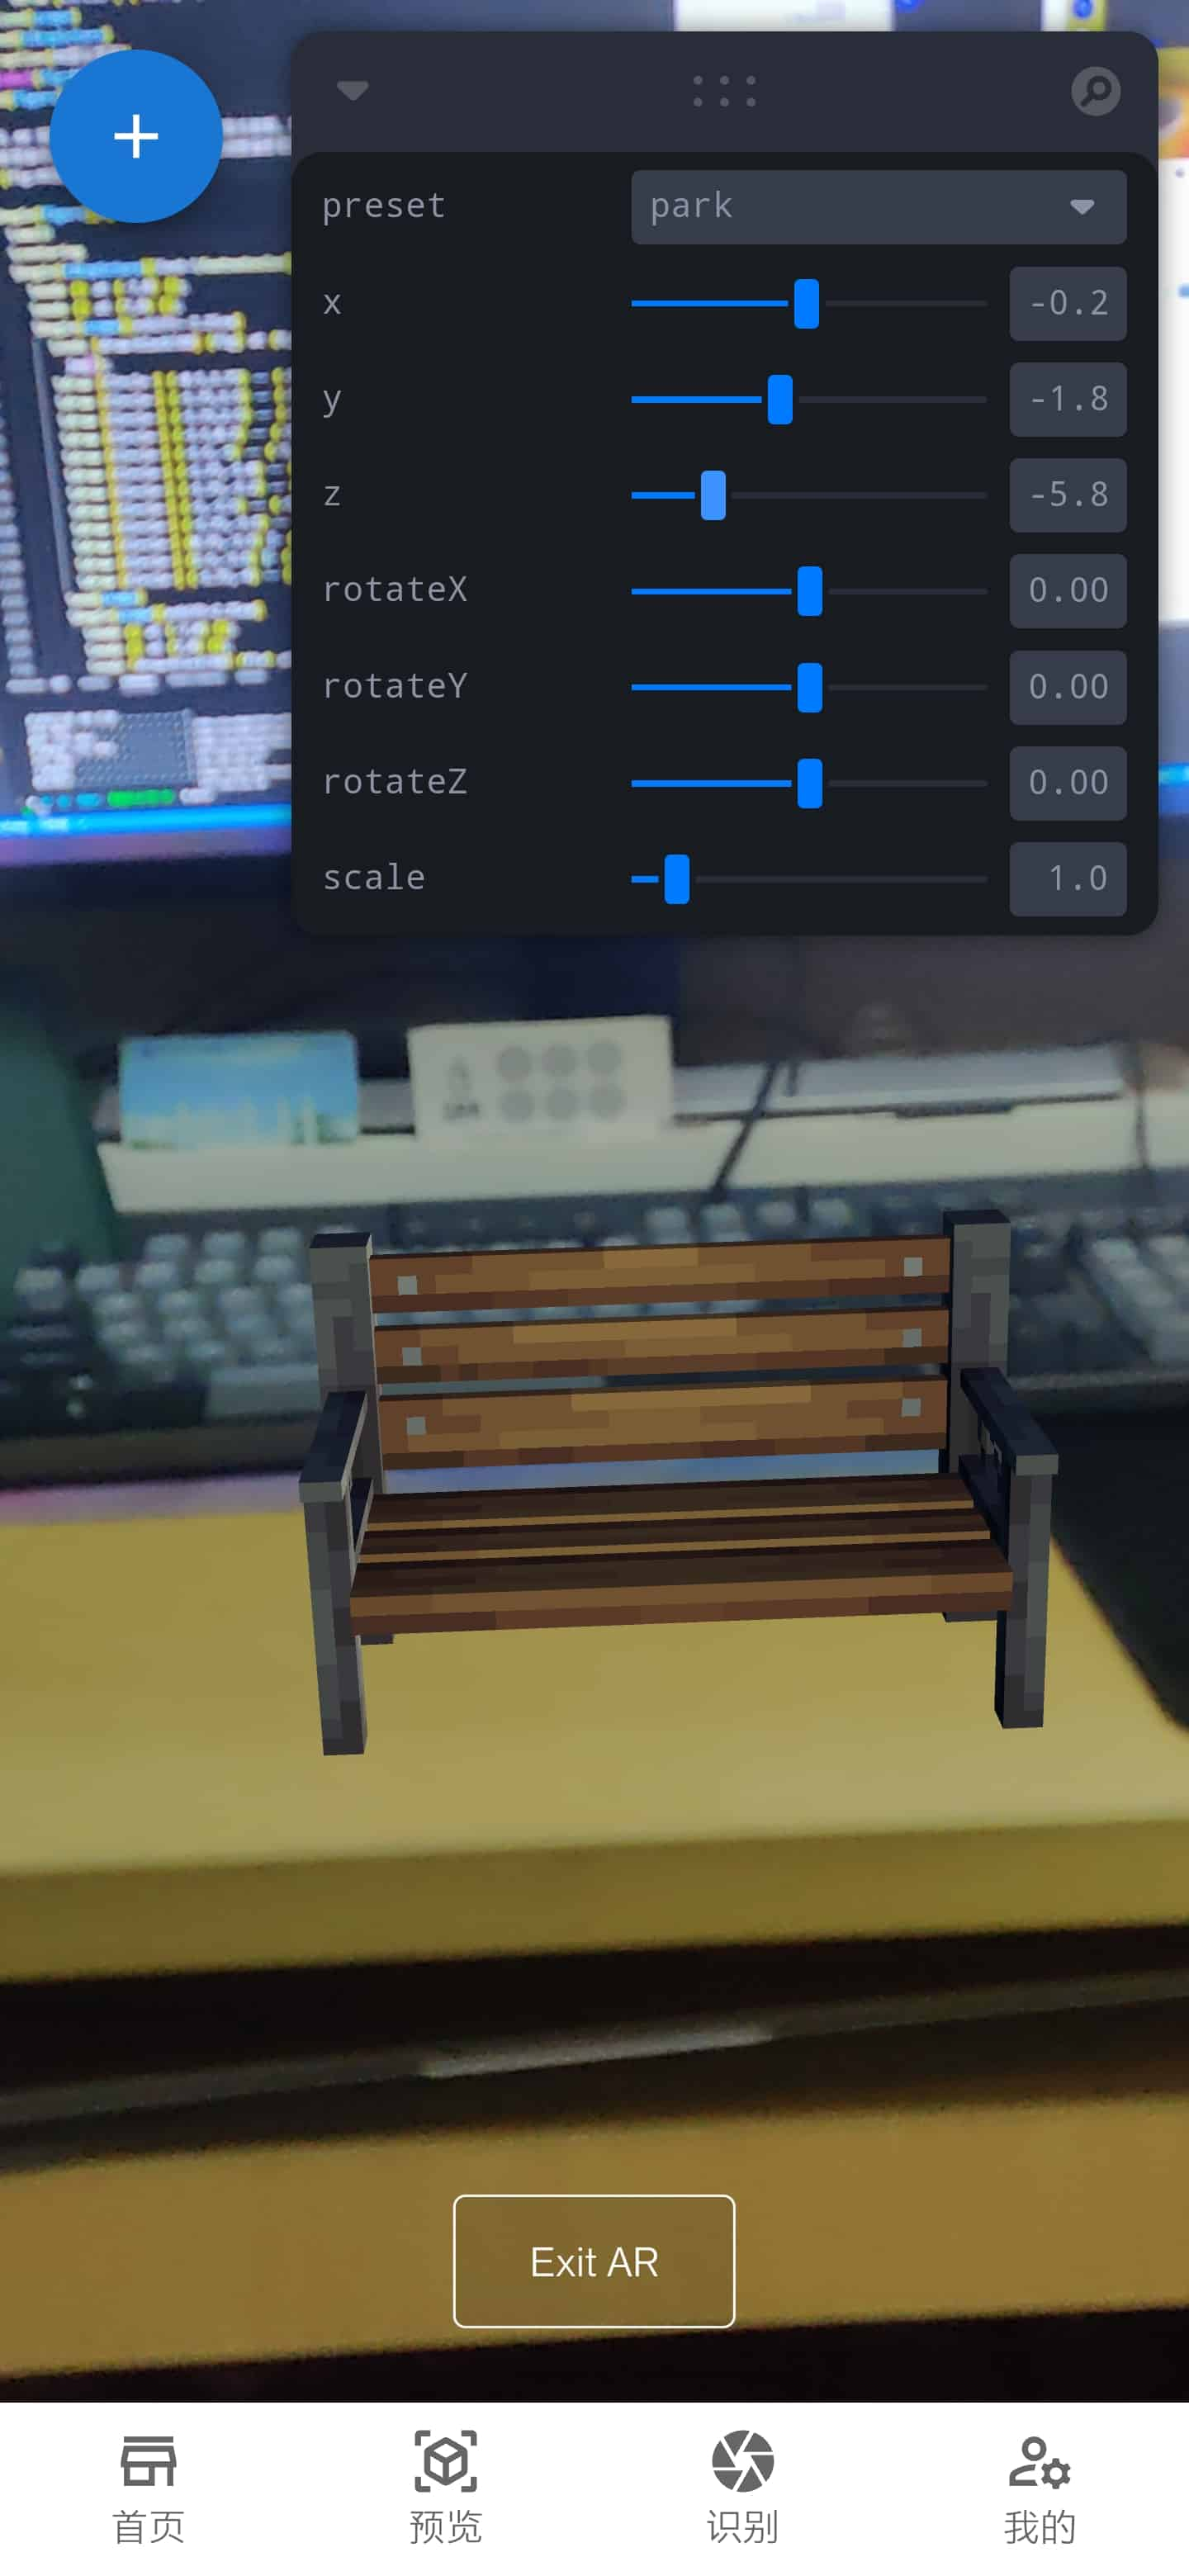
\includegraphics[width=4cm]{./figs/ar-preview-2.jpg}};
      \draw [Circle-] (1.75,3) -- (3,3) node [right] {设置模型位置参数};
      \draw [Circle-] (1.75,2) -- (3,2) node [right] {设置模型旋转参数};
      \draw [Circle-] (1.75,1.3) -- (3,1.3) node [right] {设置模型尺寸};
      \draw [Circle-] (-1.4,1) -- (3,1) node [right] {在 AR 模式中显示};
    \end{scope}
  \end{tikzpicture}
  \caption{AR预览界面}
  \label{fig:AR预览界面}
\end{figure}

进入 AR 识别界面后,系统首先会加载常规标记数据,如何通过设备地理位置在数据库中查找改区域内的标记加载。加载完所有标记数据后,系统实时匹配摄像机传输的图像,如果匹配上对应的标记,界面将弹出简略信息卡。AR 识别界面如图\ref{fig:AR识别界面}所示:

\begin{figure}[H]
  \small
  \centering
  \begin{tikzpicture}[font=\footnotesize]
    \node () at (-7,0) {};
    \node () at (7,0) {};
    \begin{scope}[xshift=-2.25cm]
      \node [draw=black!60] (fig) at (0,0) {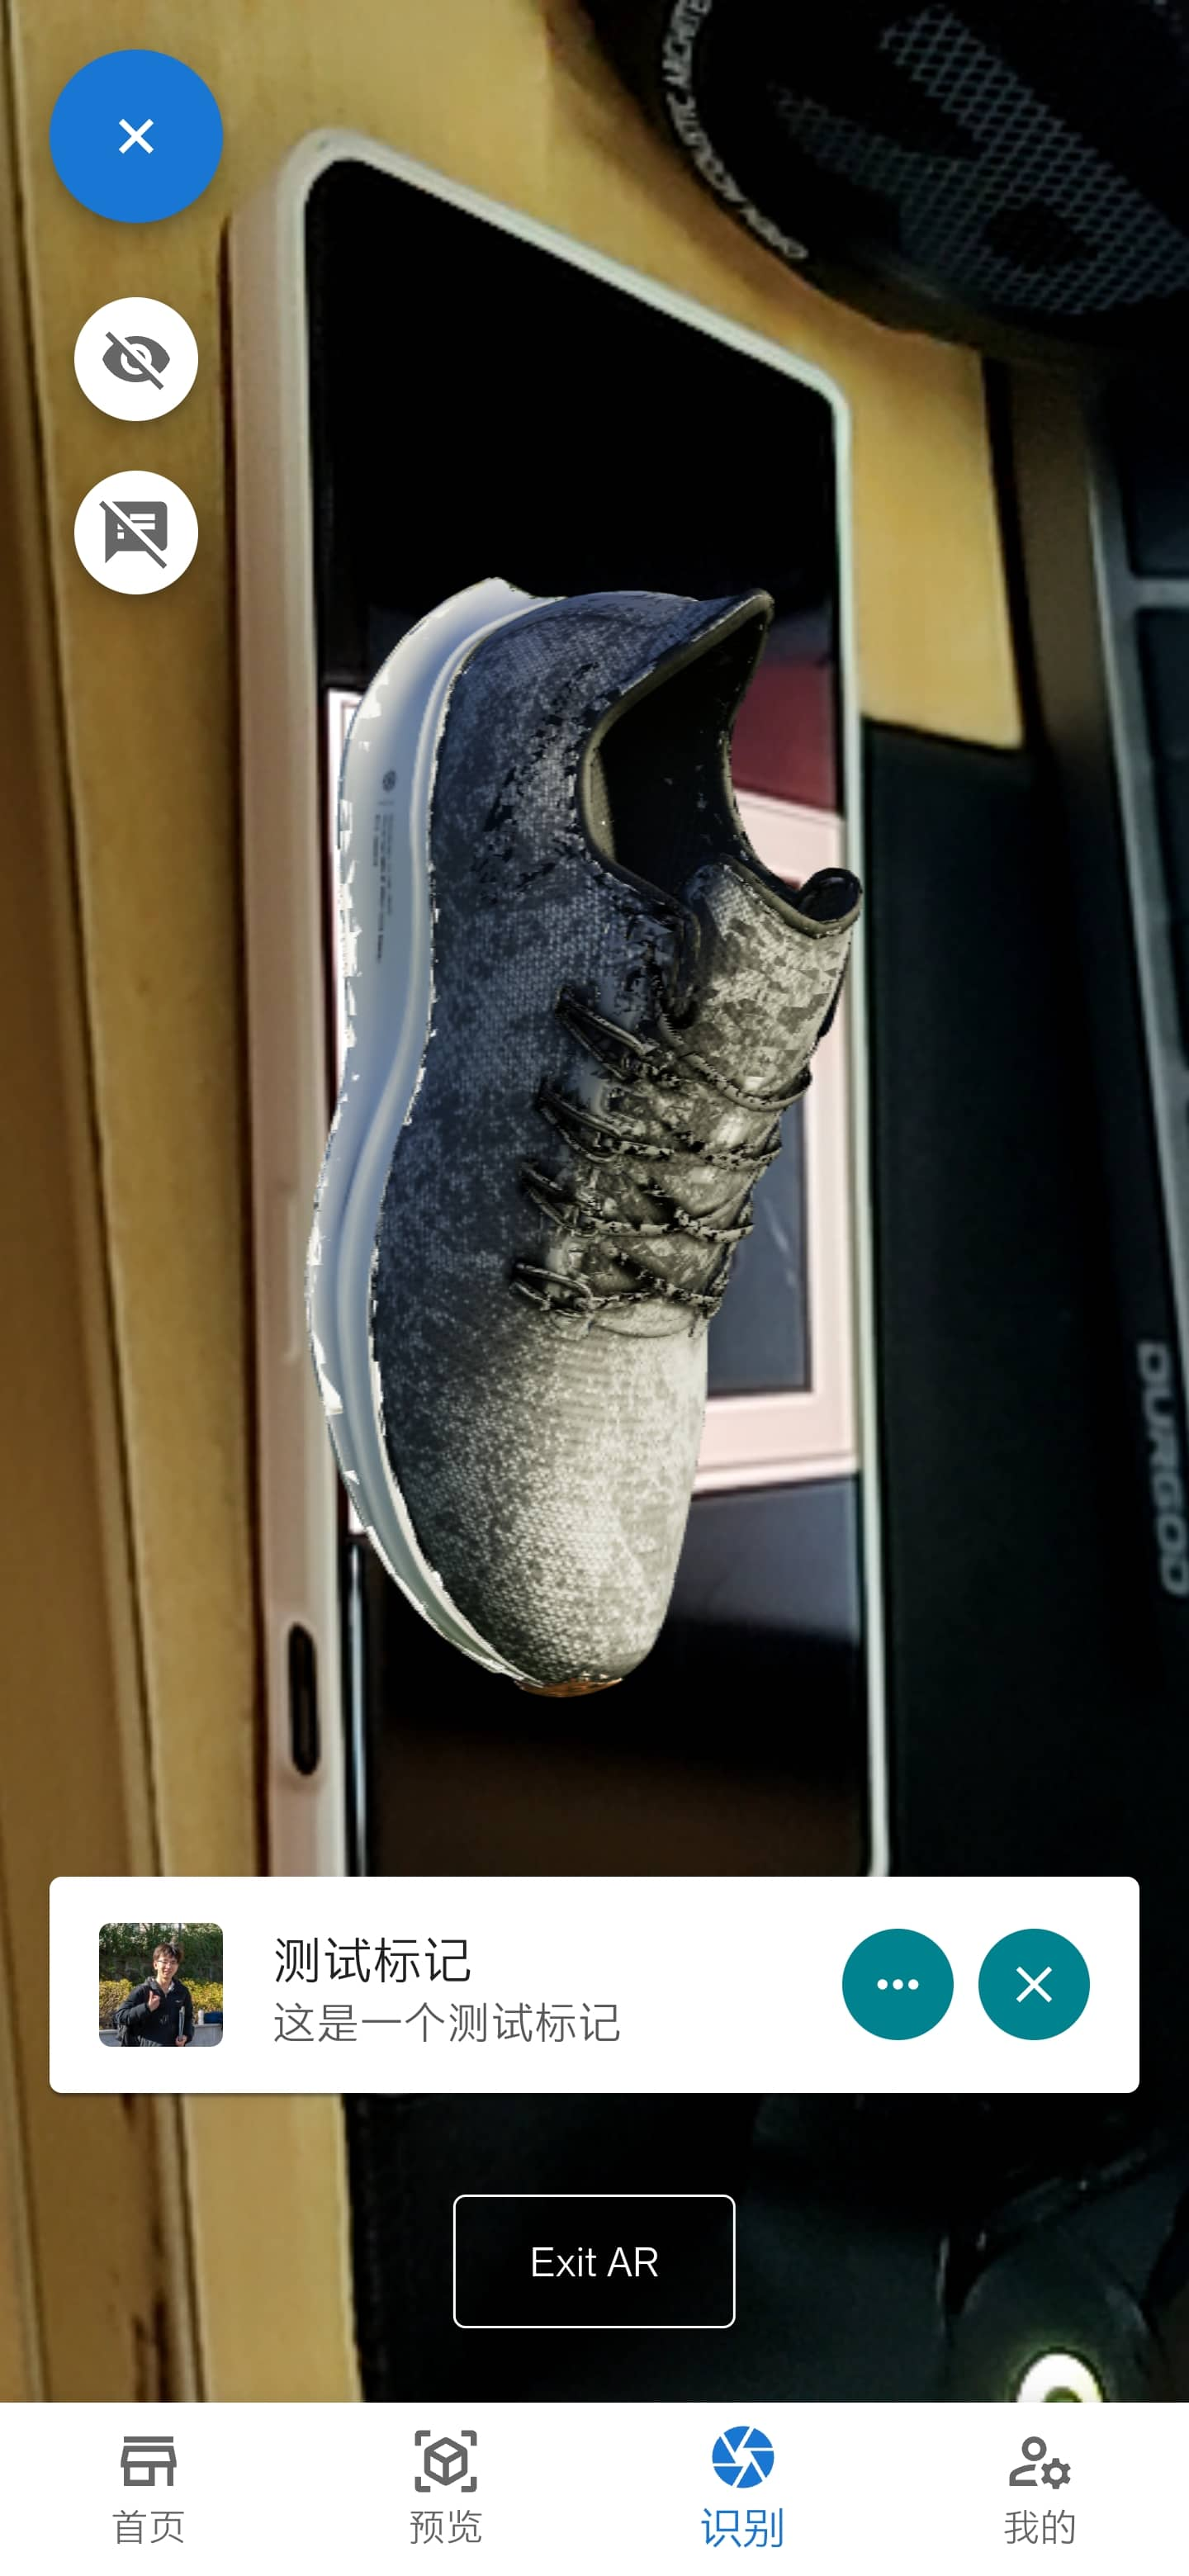
\includegraphics[width=4cm]{./figs/ar-identify.jpg}};
      \draw [Circle-] (-1.75,3.75) -- (-3,3.75) node [left] {扩展功能按钮};
      \draw [Circle-] (-1.75,3.1) -- (-3,3.1) node [left] {开关非必要组件};
      \draw [Circle-] (-1.75,2.5) -- (-3,2.5) node [left] {开关操作说明};
      \draw [Circle-] (0,0) -- (-3,0) node [left] {显示的模型};
      \draw [Circle-] (0.5,-0.5) -- (-3,-0.5) node [left] {匹配到的标记};
      \draw [Circle-] (-1.7,-2.3) -- (-3,-2.3) node [left] {标记简略信息卡};
      \draw [Circle-] (-0.25,-3.25) -- (-3,-3.25) node [left] {AR 按钮};
      \draw [Circle-] (-1.75,-4) -- (-3,-4) node [left] {其他模块链接};
    \end{scope}
    \begin{scope}[xshift=2.25cm]
      \node [draw=black!60] (fig) at (0,0) {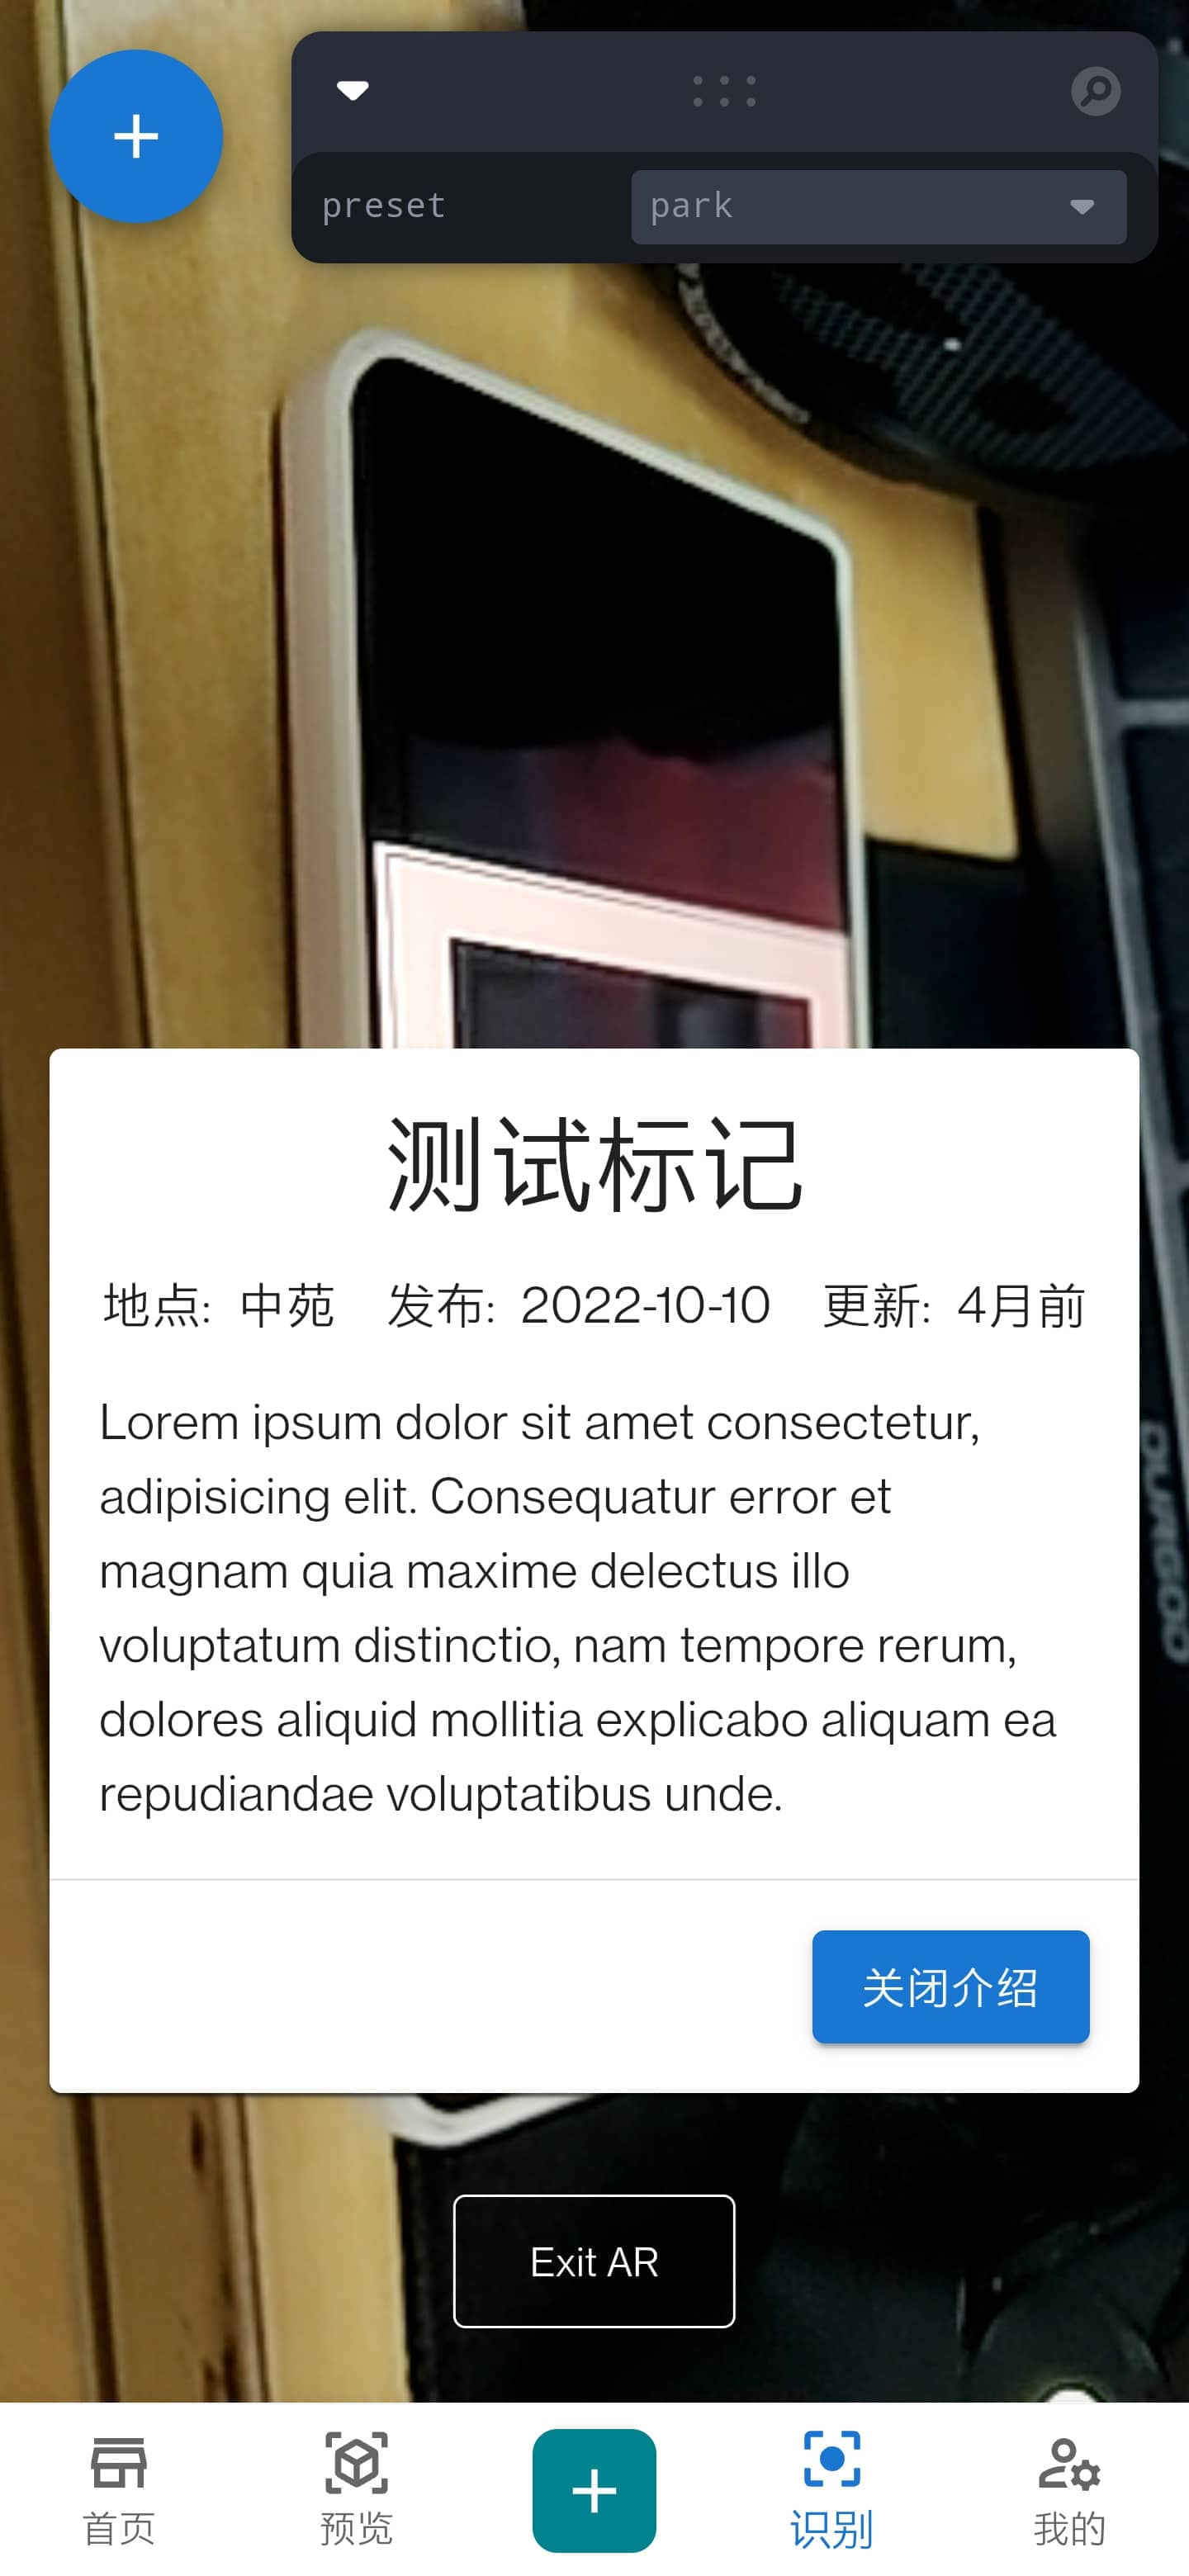
\includegraphics[width=4cm]{./figs/ar-identify-2.jpg}};
      \draw [Circle-] (0.5,4) -- (3,4) node [right] {控制板};
      \draw [Circle-] (1.75,3.6) -- (3,3.6) node [right] {设置模型背景};
      \draw [Circle-] (1.75,0) -- (3,0) node [right] {标记详细信息};
    \end{scope}
  \end{tikzpicture}
  \caption{AR识别界面}
  \label{fig:AR识别界面}
\end{figure}
\section{系统测试}

软件测试的作用是发现程序中的错误,保证软件质量,检查软件是否符合客户要求。软件测试不仅要验证软件的功能是否实现,还要验证软件在真实使用环境下能否正常运行。通过测试发现的软件问题越多,交付给用户的软件质量就越高\cite{朱少民2005软件测试方法和技术}。

\subsection{测试环境}

硬件环境:
\begin{itemize}
  \item 服务器: 本机服务器(4核8线程,24GB,10M贷款,100G 硬盘);
  \item 移动设备: 安卓手机(Snapdragon 885 处理器, Android 11 操作系统);
\end{itemize}

软件环境:
\begin{itemize}
  \item 数据库: MySQL 8.0;
  \item Java: JDK17;
  \item 浏览器: Chroe112(移动版)。
\end{itemize}

\subsection{功能测试}

\subsubsection{用户认证模块测试}

用户认证模块的功能包括用户登录,用户注册,用户信息增改。测试用例和结果如表\ref{table:用户认证模块测试用例表}所示:

\begin{table}[H]
  \centering
  \small
  \renewcommand\arraystretch{1.1}
  \caption{用户认证模块测试用例表}
  \label{table:用户认证模块测试用例表}
  \setlength{\tabcolsep}{4mm}
  \begin{tabular}{|p{4.5cm}|p{6.5cm}|p{1.5cm}|}
    \hline \textbf{功能描述} & \multicolumn{2}{l|}{用户登录,注册,信息修改} \\
    \hline \textbf{用例目的} & \multicolumn{2}{l|}{测试模块功能的可用性} \\
    \hline \textbf{前提条件} & \multicolumn{2}{l|}{用户时校园教职工或学生,在校园数据表中有记录} \\
    \hline \textbf{输出/动作} & \textbf{期望的输出/响应} & \textbf{实际情况} \\
    \hline 进入登录界面,在表单中输入用户名或邮箱以及密码。点击登录按钮。 & 前端对输入数据进行判断,根据字符关键字判断是用户名还是密码。对用户名/邮箱和密码进行格式校验。若失败,前端给出提示。若成功将数据发送到后端验证,若后端验证失败,则前端界面显示对应信息,若成功,则跳转至系统主页面。 & 符合  \\
    \hline 进入注册界面,在表单中输入工号/学号,密码等必填信息;选择性填入可填信息。点击注册按钮。 & 前端对输入数据进行格式判断。若失败,前端给出提示。若成功将数据发送到后端验证,后端查询学校用户表,根据 id 匹配注册信息,若后端验证失败,则前端界面显示对应信息,若成功,则跳转至登录页面。 & 符合  \\
    \hline 登录账户后,在``我的''界面修改个人信息,点击提交按钮。 & 前端对输入数据进行格式判断。若失败,前端给出提示。若成功将数据发送到后端验证,后端将数据存储到对应表格,若失败,前端给出错误原因,若成功,更新用户信息。 & 符合  \\
    \hline 在登录时,勾选 ``记住我'' 选项。 & 退出系统后,在一周内登录系统无需手动登录,系统自动跳转至 ``我的'' 界面。 & 符合  \\
    \hline
  \end{tabular}
\end{table}

\subsubsection{数据推送模块测试}

数据推送模块的功能包括模型推送与模型查询。测试用例和结果如表\ref{table:数据推送模块测试用例表}所示:

\begin{table}[H]
  \centering
  \small
  \renewcommand\arraystretch{1.1}
  \caption{数据推送模块测试用例表}
  \label{table:数据推送模块测试用例表}
  \setlength{\tabcolsep}{4mm}
  \begin{tabular}{|p{4.5cm}|p{6.5cm}|p{1.5cm}|}
    \hline \textbf{功能描述} & \multicolumn{2}{l|}{模型推送,模型查询} \\
    \hline \textbf{用例目的} & \multicolumn{2}{l|}{测试模块功能的可用性} \\
    \hline \textbf{前提条件} & \multicolumn{2}{l|}{用户进入系统} \\
    \hline \textbf{输出/动作} & \textbf{期望的输出/响应} & \textbf{实际情况} \\
    \hline 进入主页界面,选择分区: “为你推荐”, “最新更新”, “我的关注”。 & 前端将对应类型传输到后端,后端根据类型选择不同算法,分别采用后端三种不同的算法: 点赞数较高模型,最新更新模型,用户关注作者模型。返回数据在前端显示。 & 符合  \\
    \hline 进入主页界面,在搜索框输入模型名称,点击搜索图标。 & 前端对搜索格式进行检测,若不符合要求则给出提示信息。若符合则后端根据搜索内容查模型表模型名称,然后返回查询到的结果数据到前端能显示。 & 符合  \\
    \hline
  \end{tabular}
\end{table}

\subsubsection{数据上传模块测试}

数据上传模块的功能包括模型上传与AR标记上传。测试用例和结果如表\ref{table:数据上传模块测试用例表}所示:

\begin{table}[H]
  \centering
  \small
  \renewcommand\arraystretch{1.1}
  \caption{数据上传模块测试用例表}
  \label{table:数据上传模块测试用例表}
  \setlength{\tabcolsep}{4mm}
  \begin{tabular}{|p{4.5cm}|p{6.5cm}|p{1.5cm}|}
    \hline \textbf{功能描述} & \multicolumn{2}{l|}{模型上传,AR标记上传} \\
    \hline \textbf{用例目的} & \multicolumn{2}{l|}{测试模块功能的可用性} \\
    \hline \textbf{前提条件} & \multicolumn{2}{l|}{用户进入系统} \\
    \hline \textbf{输出/动作} & \textbf{期望的输出/响应} & \textbf{实际情况} \\
    \hline 进入上传界面,选择模型上传。在表格中填入模型 URL 等必要信息;选择性填入可选信息。点击上传按钮 & 前端对输入数据进行格式判断,对模型 URL 有效性检查。若检查失败,前端给出提示。若成功将数据发送到后端存储,后端检查是否存在相同数据,若存在返回错误信息,若存储成功,前端给出成功提示。 & 符合  \\
    \hline 进入上传界面,选择AR标记上传。在表格中填入标记 URL,标记类型等必要信息;选择性填入可选信息。点击上传按钮 & 前端对输入数据进行格式判断,对标记 URL 有效性检查。若检查失败,前端给出提示。若成功将数据发送到后端存储,后端检查是否存在相同数据,若存在返回错误信息,若成功,分别将数据存储到标记表,标记信息表。存储完成后前端给出成功提示。 & 符合  \\
    \hline
  \end{tabular}
\end{table}

\subsubsection{WebGL 模块测试}

WebGL 模块的功能包括模型显示,模型控制功能。测试用例和结果如表\ref{table:WebGL 模块测试用例表}所示:

\begin{table}[H]
  \centering
  \small
  \renewcommand\arraystretch{1.1}
  \caption{WebGL 模块测试用例表}
  \label{table:WebGL 模块测试用例表}
  \setlength{\tabcolsep}{4mm}
  \begin{tabular}{|p{4.5cm}|p{6.5cm}|p{1.5cm}|}
    \hline \textbf{功能描述} & \multicolumn{2}{l|}{模型显示,模型控制} \\
    \hline \textbf{用例目的} & \multicolumn{2}{l|}{测试模块功能的可用性} \\
    \hline \textbf{前提条件} & \multicolumn{2}{l|}{用户进入系统} \\
    \hline \textbf{输出/动作} & \textbf{期望的输出/响应} & \textbf{实际情况} \\
    \hline 进入模型预览界面,查看某个模型。 & 后端将模型信息,控制信息,环境信息等传输到前端。前端异步加载环境,模型,模型信息。用户可通过按钮切换模型摘要或模型详情模式,也可隐藏非必要卡片。 & 符合  \\
    \hline 进入模型预览界面,通过触摸操作模型,通过控制板调整数据操作模型。 & 根据用户操作,模型做出移动,缩放等响应。通过控制板的操作,场景将更换对应配置或显示新的场景。 & 符合  \\
    \hline
  \end{tabular}
\end{table}

\subsubsection{AR 模块测试}

AR 模块的功能包括AR模型预览,AR识别功能。其中 AR 识别分为图像识别与标记捕捉。测试用例和结果如表\ref{table:AR模块测试用例表}所示:

\begin{table}[H]
  \centering
  \small
  \renewcommand\arraystretch{1.1}
  \caption{AR模块测试用例表}
  \label{table:AR模块测试用例表}
  \setlength{\tabcolsep}{4mm}
  \begin{tabular}{|p{4.5cm}|p{6.5cm}|p{1.5cm}|}
    \hline \textbf{功能描述} & \multicolumn{2}{l|}{AR预览,AR识别} \\
    \hline \textbf{用例目的} & \multicolumn{2}{l|}{测试模块功能的可用性} \\
    \hline \textbf{前提条件} & \multicolumn{2}{l|}{用户进入系统} \\
    \hline \textbf{输出/动作} & \textbf{期望的输出/响应} & \textbf{实际情况} \\
    \hline 进入AR预览界面,通过摄像头在虚拟现实场景中显示模型。 & 系统获取摄像头权限并显示现实场景。将虚拟物体模型投射到真实场景中提供预览功能。 & 符合  \\
    \hline 进入AR预览界面,通过操纵轴触摸操作模型位置,控制模型进行旋转。 & 模型根据用户触摸操作做出响应,对应位置或旋转信息改变并显示在界面上。 & 符合  \\
    \hline 进入AR预览界面,通过控制板改变模型或场景信息。 & 模型或场景根据改变的信息实时应用,并显示在界面上。 & 符合  \\
    \hline 进入AR识别界面,摄像头对准可识别的图像,等待系统响应。 & 系统匹配到图像信息后,如果存在预定义的 3D 模型,则显示在界面上;如果存在标记信息,则界面弹出简要标记卡片。 & 符合  \\
    \hline 进入AR识别界面,摄像头对准可识别的标记,等待系统响应。 & 系统匹配到标记信息后,如果存在预定义的 3D 模型,则显示在界面上;如果存在标记信息,则界面弹出简要标记卡片。 & 符合  \\
    \hline 弹出简要标记卡片后点击查看详细信息。 & 系统弹出详细信息卡,同时停止图像识别功能,在关系信息卡后重新进行图像识别。 & 符合  \\
    \hline
  \end{tabular}
\end{table}

\subsection{性能测试}

在性能测试过程中,针对需求分析中的非功能需求,对系统进行性能测试。具体测试方法为采用测试设备对系统各个功能接口同时进行测试,单个接口的测试量为 20 次,同类接口总体测试量大于 100,获得测试结果后取平均响应时间。测试用例和结果如表\ref{table:性能测试表}所示。

\begin{table}[H]
  \centering
  \small
  \renewcommand\arraystretch{1.1}
  \caption{性能测试表}
  \label{table:性能测试表}
  \setlength{\tabcolsep}{4mm}
  \begin{tabular}{|p{4.5cm}|p{4cm}|p{4cm}|}
    \hline \textbf{输入动作} & \textbf{期望的输出/响应} & \textbf{实际情况} \\
    \hline 切换系统界面 & 界面加载时间 <1s, 网络加载时间 <2s & 界面加载时间 <0.5s, 网络加载时间 <2s  \\
    \hline 点击按钮,弹出弹框并显示内容 & 界面加载时间 <1s & 界面加载时间 <0.5s  \\
    \hline 主页选择不同数据分析,等待返回内容 & 界面加载时间 <2s & 界面加载时间 <1.5s  \\
    \hline 主页搜索模型,等待返回内容 & 界面加载时间 <2s, 网络加载时间 <2s & 界面加载时间 <2s, 网络加载时间 <1s  \\
    \hline 模型预览界面加载场景,并开始异步加载模型 & 界面加载时间 <2s, 网络加载时间 <2s & 界面加载时间 <1s, 网络加载时间 <1s  \\
    \hline AR 预览界面开启摄像头,开始异步加载模型 & 界面加载时间 <2s, 网络加载时间 <2s & 界面加载时间 <1s, 网络加载时间 <1s  \\
    \hline AR 识别界面开启识别图像信息 & 界面加载时间 <2s, 网络加载时间 <2s & 界面加载时间 <1.5s, 网络加载时间 <2s  \\
    \hline AR 识别界面开启识别标记信息 & 界面加载时间 <1.5s, 网络加载时间 <2s & 界面加载时间 <1s, 网络加载时间 <2s  \\
    \hline
  \end{tabular}
\end{table}

\subsection{兼容性测试}

本部分对主流浏览器做兼容性测试,测试系统的功能,页面布局是否正常显示。测试结果如表\ref{table:兼容性测试表}所示:

\begin{table}[H]
  \centering
  \small
  \renewcommand\arraystretch{1.1}
  \caption{兼容性测试表}
  \label{table:兼容性测试表}
  \setlength{\tabcolsep}{4mm}
  \begin{tabular}{|p{6.5cm}|c|c|c|}
    \hline \textbf{测试目的} & \textbf{测试目标} & \textbf{期望结果} & \textbf{实际情况} \\
    \hline 检查页面布局,WebGL 模型显示效果,AR 预览与识别效果 & Chrome & 显示正常,功能正常 & 符合  \\
    \hline 检查页面布局,WebGL 模型显示效果,AR 预览与识别效果 & Edge & 显示正常,功能正常 & 符合  \\
    \hline 检查页面布局,WebGL 模型显示效果,AR 预览与识别效果 & Firefox & 显示正常,功能正常 & 符合  \\
    \hline
  \end{tabular}
\end{table}
\section{总结}

本文以 WebGL 与 AR 技术为核心,介绍了 AR 交互系统的研究现状与研究意义,探索 AR 系统在 Web 领域的可行性,在完成技术选择,需求分析,系统整体设计,模块详细设计后,实现了基于 WebGL 的校园交互系统,并通过系统测试验证了系统的可用性,稳定性。系统以移动端浏览器为载体,调用操作系统底层 AR 服务,通过现有的 WebGL 与 AR 技术实现了模型预览,AR 预览,AR 识别等核心功能。

本系统的主要成果包括:
\begin{itemize}
  \item 基于 AR.js 提供的标识识别与图像识别算法,开发出了 AR 识别系统,能够对校园特定场景与物体进行识别并提供对应信息。
  \item 基于 three.js 技术,开发了 Web 端三维模型显示系统,并提供了一定的交互功能。结合 AR.js 基础开发了 AR 交互功能。给用户提供了一种更生动,更直观的交互方式。
  \item 基于 React,MaterialUI 技术,搭建了有好的前端系统,以此为依托开发了核心的 WebGL 与 AR 功能。用户无需下载任何应用即可访问系统。
  \item 基于 SpringBoot 技术搭建了后端系统,向前端提供稳定数据。
\end{itemize}

本文研究的 AR 系统可以提供更完善的预览服务,基于用户更丰富的视觉体验,本系统可拓展到教育,建筑,工业等各个领域,并于已有系统结合,有效提高工作,学习效率。本系统完全基于开源框架,且基于 Web 系统。决绝传统 AR 服务闭源,兼容性差等特点。

本系统同样存在部分问题,系统依赖于高性能智能设备,需要设备提供 AR 服务,需要用户具备一定的 3D 模型知识。


%%%%%%%%%% 封面目录摘要 %%%%%%%%%%

%%%%%%%%%% 正文 %%%%%%%%%%
% TIPS: 可以为每一章节在 body 文件夹内创建一个 .tex 文件,并以下述方式引入,也可以直接写在本文件中(不推荐)
% \input{body/intro.tex}
% \input{body/nuistcommand.tex}
% \input{body/math.tex}
% \input{body/figs.tex}
% \input{body/table.tex}
% \input{body/code.tex}
% \input{body/ref.tex}
%%%%%%%%%% 正文 %%%%%%%%%%

%%%%%%%%%% 参考文献 %%%%%%%%%%
\bibliography{bibliography}
\clearpage % 输出所有剩余的浮动体(图片、表格等),另起一页
%%%%%%%%%% 参考文献 %%%%%%%%%%

%%%%%%%%%% 附录(可选) %%%%%%%%%%
% \input{body/appendix.tex}
%%%%%%%%%% 附录(可选) %%%%%%%%%%

%%%%%%%%%% 致谢 %%%%%%%%%%
% TIPS: \thanking 命令中包含了 \clearpage
\thanking
{
    时光白驹过隙,我在南信大已经学习了四年,在这段学习生涯中,我要向我的母校表达最深切的谢意,感谢学校在我大学期间为我提供的一流教育资源和培养机会。在这里,我不仅仅获得了专业知识和技能,还收获了友情和人生经验。

    其次,我要感谢我的导师对我的指导和支持。导师的悉心教诲和鼓励,对我完成毕业设计起到了至关重要的作用。导师不仅仅在学术研究方面给予我指导,还关心我的个人成长和发展,给了我很多宝贵的建议和启示。
    
    最后,我要感谢所有在我大学四年期间给予我帮助和支持的人。我的家人、朋友和同学们一直陪伴着我,给予我鼓励和支持。在这里,我要向你们表达最真挚的谢意和感激之情。
}
%%%%%%%%%% 致谢 %%%%%%%%%%

\end{document}
